\chapter{TEPX luminometer for HL-LHC}  %Title of the First Chapter

\ifpdf
    \graphicspath{{Chapter7/Figs/Raster/}{Chapter7/Figs/PDF/}{Chapter7/Figs/}}
\else
    \graphicspath{{Chapter7/Figs/Vector/}{Chapter7/Figs/}}
\fi

The Phase II upgrade of the CMS Tracker is a crucial project undertaken to maintain the effectiveness of the CMS experiment during the High Luminosity LHC (HL-LHC) phase, which is expected to start in 2029 \cite{CERN2022}. The HL-LHC will significantly increase the instantaneous luminosity, leading to a higher number of proton-proton collisions per bunch crossing. Instantaneous luminosity will increase to an unprecedented value of $7.5 \times 10^{34} cm^{-2} \: s^{-1}$ which corresponds to 200 proton-proton collisions per bunch crossing. This higher collision rate poses several challenges, including increased radiation levels, higher data rates, and more complex event environment. Run 2 pixel detector will not be able to handle these extreme radiation environment, resolve nearby particle tracks and operate properly to give a reliable estimate of the instantaneous luminosity for such a high pileup. That is why it will be replaced by a new pixel detector. The Phase II upgrade of the CMS tracker comprises of two main components: the Inner Tracker (IT) and the Outer Tracker (OT) \cite{RoyChowdhury:2729279}. The Inner Tracker consists of three main sub-components: the Tracker Endcap Pixel detector (TEPX), the Tracker Forward Pixel detector (TFPX), and the Tracker Barrel Pixel (TBPX) detector as shown in Fig. \ref{fig:Innertracker} \cite{CERN-LHCC-2017-009}.  %The Outer Tracker is responsible for detecting charged particles in the outer region of the CMS detector. It consists of two key subsystems: the silicon strip tracker and the silicon macro pixel tracker \cite{RoyChowdhury:2729279}.

Data Acquisition (DAQ) system for the Phase II CMS Tracker must handle the increased data rates and complexity associated with the HL-LHC. The HL-LHC is expected to achieve a peak luminosity which is around 5-7 times higher than the current LHC design luminosity which the DAQ system must handle. The upgraded CMS Tracker will generate a large amount of data due to the increased granularity of the pixel and strip sensors. The data rates from the tracker modules are expected to be several terabits per second (Tbps) during the HL-LHC operation. The Level-1 Trigger system in the Phase II Upgrade is designed to accept events at a rate of up to 750 kHz. The DAQ system must handle the transmission of trigger primitives to the Level-1 Trigger system and buffer the full event data until the trigger decision is made. %The high-speed optical links used for data transmission between the Front-End Electronics (FEE) and off-detector electronics are expected to operate at data rates of 10-25 Gbps or higher to handle the large data volumes generated by the upgraded tracker.
In the Inner Tracker readout system, control signals are sent to the it at 160 Mb/s to coordinate its detection processes. It, in turn, outputs data at 1.28 Gb/s per chip to the LpGBT, which acts as a data consolidator for up to three chips. This data is then relayed optically to the DTC board, which operates a bidirectional data exchange: 2.5 Gb/s optical down-links channel control information back to the Inner Tracker, while 10 Gb/s up-links carry processed readout data and monitoring details to the DAQ and control system. Moreover, the DTC can interface with a Lumi processor via an optional link, designed for a substantial data transfer rate of approximately 4x25 Gb/s, to handle specialized luminosity data processing. Finally, the DAQ and control system, which receives the comprehensive data at a substantial rate of 25 Gb/s, undertakes the final processing and storage of data.


The TBPX occupies the central region along the \( z \)-axis from 0 to just below 300~mm, employing \( 1 \times 2 \) modules (modules with two readout chips) and \( 2 \times 2 \) modules (modules with four readout chips) arranged in four layers parallel to the beam. The TFPX extends from approximately 250~mm to 1400~mm in the \( z \)-direction, with \( 1 \times 2 \) and \( 2 \times 2 \) modules. The TEPX covers a range from about 1700~mm to over 2600~mm and includes  \( 1 \times 2 \) and \( 2 \times 2 \) modules. Collectively, these sub-detectors boast around 1.947 billion pixels across 13,488 pixel chips, spanning a silicon area of 4.87 square meters.

The TEPX consists of four double-disk per side with each double-disk consisting of five rings of modules as shown in Fig. \ref{fig:Innertracker_40}. The rings have 20, 28, 36, 44 and 48 modules respectively.
The first two inner rings are equipped with \(1 \times 2\) modules, while the more extensive \(2 \times 2\) modules are mounted on the three outer rings. This design is further enhanced by the arrangement of modules in four layers as shown in Fig. \ref{fig:Innertracker_41}. This allows for modules to be mounted on both the front and back sides of a disk, creating an overlap in the r-\(\phi\) direction. By mounting modules at varying radii on the two disk that form each double-disk, overlap in the radial direction (r) is also accomplished. TEPX will have better radiation tolerance, increased granularity, improved two-track separation, improved estimation of hit rate and statistical precision, extending tracking acceptance beyond $|\eta|=4$.

%One double disk has four surfaces with +Z side consisting of modules with even module number in front layers (L1 $\&$ L2) and modules with odd module number in back layers (L3 $\&$ L4) from Ring 1 to Ring 4 and for Ring 5, modules with odd module number in front layers and modules with even module number in back layers as shown in Fig.   \ref{fig:Innertracker_41}.

%For -Z side, four surfaces contain modules with odd module number in front layer and modules with even module number in back layer from Ring 1 to Ring 4 and for Ring 5, modules with even module number in front layer and modules with odd module number in back layer.

%TEPX will have better radiation tolerance, increased granularity, improved two-track separation, improved estimation of hit rate and statistical precision, extending tracking acceptance beyond $|\eta|=4$. Collectively, these sub-detectors boast around 1.947 billion pixels across 13,488 pixel chips, spanning a silicon area of 4.87 square meters.

%The Outer Tracker is designed for tracking particles over extended radii with six "barrel" layers for \( |z| < 1200 \)~mm and five "endcap" double-discs for \( 1200 \text{~mm} < |z| < 2700 \)~mm. The modules are radially placed from about 21~cm to 112~cm. It features 2S modules with 2032 strips each and PS modules with 1920 strips and 30,720 macro-pixels of about 1.5~mm size. The PS modules are located in the innermost three layers (200--600~mm radial distance) for precise \( z \)-coordinate measurement, while the 2S modules are positioned in the outer layers beyond 600~mm, with various strip lengths to cater to different tracking requirements.

\begin{figure}[H]
  \centering
  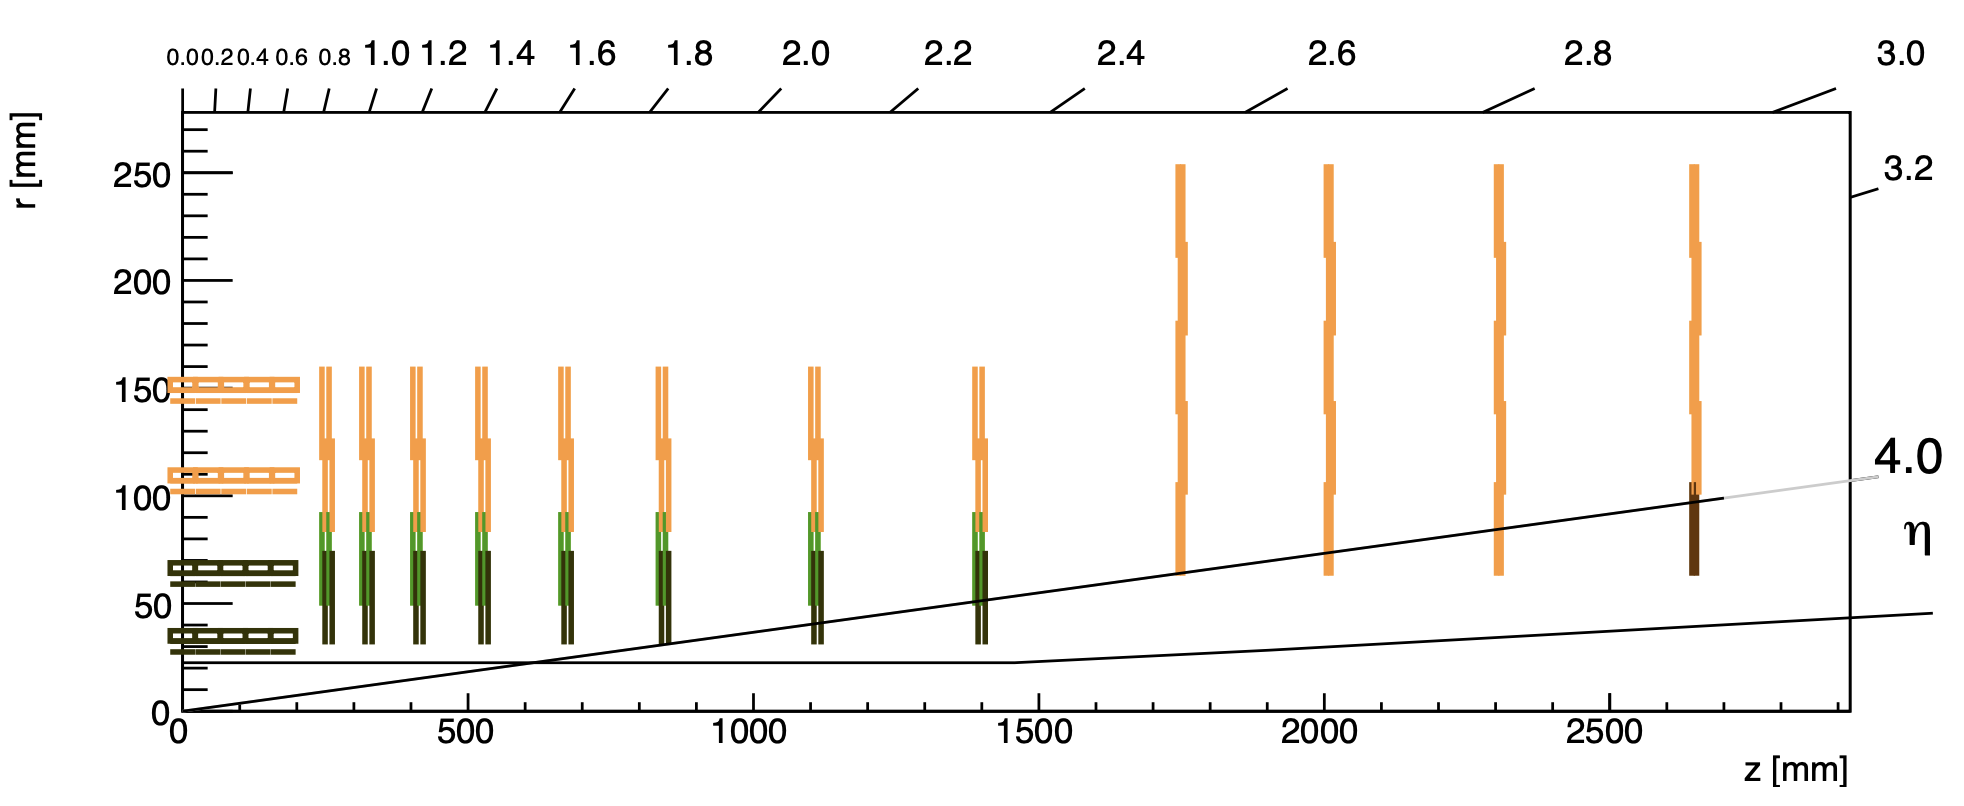
\includegraphics[width=1 \columnwidth]{ashish_thesis/it_newgeometry_.png}
  \caption[Phase II CMS Inner Tracker]{ \onehalfspacing A layout of the CMS Phase II Inner Tracker showing four TEPX disks, eight TFPX disks and four TBPX layers \cite{Collaboration:275907420}.}
  \label{fig:Innertracker}
\end{figure}

\begin{figure}[H]
  \centering
  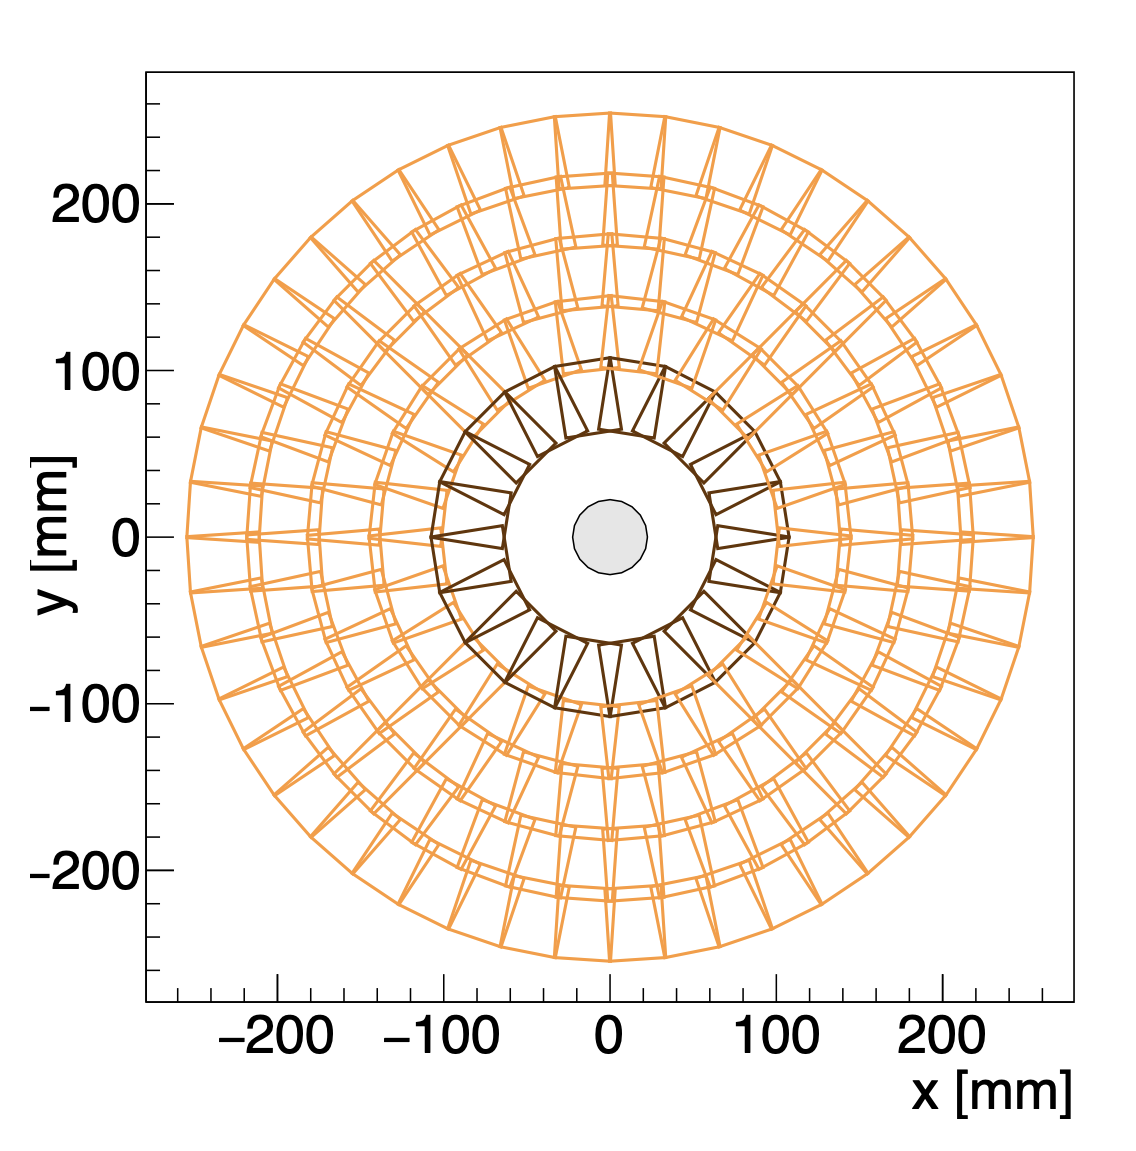
\includegraphics[width=0.5 \columnwidth]{ashish_thesis/tepx_DD.png}
  \caption[X-Y view of TEPX double-disk]{ \onehalfspacing View of one TEPX double-disk in the $r-\phi$ plane; individual pixel modules on two planes (double-disk) and five rings are outlined by yellow rectangles. %The planes are separated in z by about 1 cm. The first plane holds modules on both front and back faces, with alternating rings to cover the gaps in r; the second plane holds modules in the same way as the first plane, but with an offset in $\phi$ to cover the gaps in $\phi$.
  }
  \label{fig:Innertracker_40}
\end{figure}


\begin{figure}[H]
  \centering
  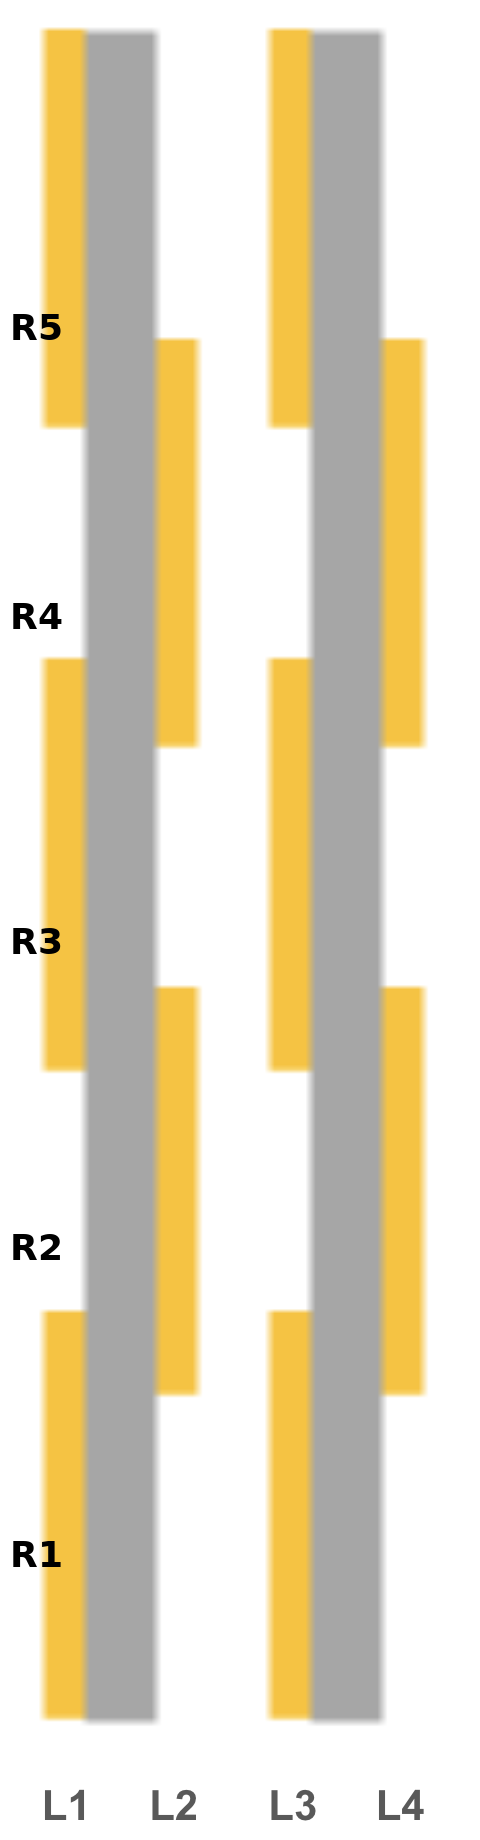
\includegraphics[width=0.1 \columnwidth]{ashish_thesis/edited_tepx_alllayer_v5.png}
  \caption[R-Z view of TEPX double-disk]{ \onehalfspacing R-Z view of the TEPX double-disk showing the four layers of modules L1, L2, L3 and L4. Layer 1 and 3 has Ring 1, 3 and 5 modules, Layer 2 and 4 has Ring 2 and Ring 4 modules. The planes are separated in z by about 1 cm. The first plane holds modules on both front and back faces, with alternating rings to cover the gaps in r; the second plane holds modules in the same way as the first plane, but with an offset in $\phi$ to cover the gaps in $\phi$.}
  \label{fig:Innertracker_41}
\end{figure}

\section{TEPX Luminometer}

TEPX is designed to function as a high-precision online bunch-by-bunch luminometer, primarily uses pixel cluster counting for luminosity measurement, a method involving the detection and counting of pixel clusters formed by charged particles from the proton collisions. Additionally, TEPX benefits from coincidence counting due to overlapping modules which enhances accuracy and enables systematic studies. %Positioned as part of the forward extension of the Inner Tracker detector,
TEPX features a sophisticated dedicated trigger system for sampling all relevant bunch crossings in an unbiased manner. This system operates at a baseline trigger rate of 75 kHz, which is 10$\%$  of the 750 kHz allocated for physics data. %In terms of data acquisition,
TEPX adapts to different operational conditions: during standard physics runs, it maintains a baseline luminosity trigger rate of 75 kHz, while during van der Meer (vdM) scans, this rate can significantly increase, potentially up to 1 MHz \cite{Collaboration:2706512}. %TEPX readout rate (E-link speed) is estimated to be approximately 1330 Gbps at a pileup of 200  \cite{Collaboration:2706512}.
%The DAQ system of TEPX is designed to handle substantial data rates, with link bandwidth requirements varying from about 79.2 Gb/s at a trigger rate of 825 kHz during nominal physics operations to up to 24 Gb/s at the standard rate of 75 kHz  \cite{Collaboration:2706512}.

TEPX Disk 4 Ring 1 (D4R1) is located in the innermost ring of the last double-disk of the TEPX, is exclusively designed for measuring luminosity and beam-induced background (BIB). D4R1 is optimally placed due to its low radius, large active area, and high z position, making it highly efficient for these measurements. The D4R1 operational model is distinct from the rest of TEPX \cite{Haranko2023}. It employs the entire available trigger rate and readout bandwidth, which varies based on operational mode. This capability ranges from a trigger rate of 825 kHz (similar to the rest of TEPX) up to several MHz, limited by readout bandwidth and the available e-link capacity. In nominal physics conditions, the baseline trigger rate for D4R1 is 825 kHz, while in van der Meer (vdM) conditions, it is 2 MHz, with the potential to reach between 5 and 10 MHz in certain scenarios. 

%A significant advantage of D4R1 is its independence from the CMS central services, particularly during special beam conditions like machine development and LHC ramp. This independence allows for luminosity measurements and BIB analysis even outside stable beams, providing vital data to improve accelerator performance. D4R1 operates on the LHC clock, enabling it to measure BIB throughout the full LHC machine cycle, including during ramp phases when the radio frequency clock, and consequently the bunch clock, increases significantly. To maintain this independent yet synchronized operation with the rest of CMS, a special clocking scheme is employed. This scheme involves the BRIL trigger board (BTB) and a Data Transmission Hub (DTH), which interfaces with the central TCDS2 system to receive all necessary signals, including clocks, triggers, and synchronization commands. This setup ensures that D4R1 can operate on the LHC clock while remaining synchronized with CMS during various operational phases, including the ramp and stable beams.

%The Outer Tracker (OT) Layer 6 of the CMS will play a pivotal role in luminosity measurement, trigger, and data acquisition for the CMS experiment. It is designed to perform bunch-by-bunch measurements. This is achieved by utilizing a technique called "coincidence counting," which involves detecting two-hit coincidences on two closely spaced silicon sensors, also known as "stubs." This system operates at the full 40 MHz bunch-crossing frequency, which is essential for capturing the high-frequency data required for accurate and timely analysis.

%As part of the forward extension of the Inner Tracker detector, TEPX features an advanced dedicated trigger system. This system is crucial for sampling all relevant bunch crossings in an unbiased manner, operating at a trigger rate of 75 kHz, which constitutes 10$\%$ of the 750 kHz allocated for physics. For luminosity measurements, TEPX primarily employs pixel cluster counting, a technique that counts the number of pixel clusters formed due to particle interactions within the detector. Additionally, TEPX is capable of coincidence counting in overlapping modules, enhancing measurement accuracy and aiding in systematic studies. This method counts coincident events in neighboring modules. In terms of data acquisition, TEPX adapts to varying operational conditions: during standard physics runs, it manages a baseline luminosity trigger rate of 75 kHz, while during van der Meer (vdM) scans, this rate can increase considerably, potentially up to 1 MHz. The DAQ system of TEPX is designed to handle substantial data rates, with link bandwidth requirements varying from about 79.2 Gb/s at a trigger rate of 825 kHz during nominal physics operations to up to 24 Gb/s at the standard rate of 75 kHz. This sophisticated combination of trigger systems, pixel cluster counting, and adaptable DAQ capabilities highlights TEPX's vital role in accurate luminosity measurement across different CMS operational scenarios.

\begin{comment}

 with Disk 4 Ring 1 operating as an independent luminosity measurement device \cite{Collaboration:2706512}. 
\begin{enumerate}

\item Inner Tracker: The Inner Tracker is the innermost part of the CMS Tracker, closest to the collision point. It is designed to provide high-resolution position measurements of charged particles in a high-density environment, as well as excellent radiation tolerance. The Inner Tracker is crucial for the precise determination of the primary and secondary vertices (interaction points) and the accurate reconstruction of decay paths of short-lived particles. The Inner Tracker of the CMS experiment during the Phase II Upgrade will consist of three main subcomponents: TEPX (Tracker Endcap Pixel), TFPX (Tracker Forward Pixel), and TBPX (Tracker Barrel Pixel) \cite{CERN-LHCC-2017-009}. These subsystems together form the new high-resolution, highly granular, and radiation-tolerant pixel tracking system.

\begin{itemize}

\item TBPX (Tracker Barrel Pixel): The TBPX subsystem is located in the central region of the Inner Tracker, arranged in a barrel geometry around the beam axis. It consists of several concentric cylindrical layers of high-resolution pixel sensors, providing precise measurements of charged particle trajectories in the xy-plane. The upgraded TBPX will feature higher granularity pixel sensors to better handle the increased event rates and radiation levels expected during the HL-LHC era.

\item TFPX (Tracker Forward Pixel): The TFPX subsystem covers the forward regions of the Inner Tracker, extending the coverage in the pseudorapidity ($\eta$) direction. Like the TBPX, it consists of high-resolution pixel sensors, arranged in multiple concentric discs around the beam axis. The TFPX will provide precise position measurements for charged particles in the forward and backward regions, complementing the coverage provided by the TBPX.

\item TEPX (Tracker Endcap Pixel): The TEPX subsystem is located further out in the forward and backward regions, surrounding the TFPX subsystem. It consists of additional concentric discs of pixel sensors, further extending the tracking coverage in the pseudorapidity direction. The TEPX helps to ensure efficient tracking performance in the high-$\eta$ regions, where the particle density is lower compared to the central region.

\end{itemize}

\item Outer Tracker: The Outer Tracker is designed to provide additional tracking points for charged particles as they traverse through the CMS detector. This extra information helps improve the overall track reconstruction accuracy and efficiency. In the Phase II Upgrade, the Outer Tracker will be based on the novel concept of "Tracker-Trigger," which combines tracking and triggering functionalities.

\begin{itemize}

\item In the upgraded Outer Tracker, silicon strip sensors will be used to form "trigger primitives" - early-stage track candidates - that are passed to the Level-1 Trigger system. This approach helps to reduce the data volume and allows the CMS experiment to maintain its excellent physics performance in the face of increased event rates.

\item The Outer Tracker will consist of multiple layers of strip sensor modules, organized in barrel and endcap regions. The sensor modules will be connected to custom-designed readout electronics that process the data in real-time and transmit the trigger primitives to the Level-1 Trigger system.

\end{itemize}

\item The CMS Tracker's Phase II upgrade includes the Timing Layer, equipped with Low Gain Avalanche Detectors (LGAD) to improve time measurement of charged particles. This enhancement helps distinguish particles from different vertices, reducing pileup in event reconstruction. LGADs, with their charge amplification capability, offer superior time resolution. Charged particles generate electron-hole pairs in the LGAD sensor, which are then amplified and collected quickly for improved timing accuracy. The system aims for a 30-40 picosecond time resolution, enhancing particle identification and handling pileup effects. Covering a pseudorapidity range of $|\eta|$ < 2.5, the Timing Layer has a lightweight, radiation-tolerant support structure with efficient cooling, ensuring reliable performance.

  %Timing layer is a new addition to the CMS Tracker during the Phase II upgrade, designed to provide precise time measurements of charged particles passing through the detector. These measurements help in distinguishing between particles originating from different vertices in the same event and reducing the impact of pileup on event reconstruction. The timing layer uses Low Gain Avalanche Detectors (LGAD) as the active material. LGADs are a type of silicon sensor that incorporates a multiplication layer to generate an avalanche of charge carriers when a charged particle passes through the detector. This multiplication process results in a faster signal response and improved time resolution compared to traditional silicon sensors. When a charged particle traverses the timing layer, it creates electron-hole pairs in the LGAD sensor. The electric field within the sensor separates these charge carriers, and the multiplication layer amplifies the signal through the avalanche process. The charge carriers generated by the passing particle are collected by the pixel or strip electrodes on the LGAD sensor. These electrodes are designed to minimize the signal collection time, further improving the timing layer's time resolution. The electrical signals from the LGAD sensors are processed by custom-designed front-end electronics. These electronics amplify, shape, and digitize the signals, converting them into a form suitable for further processing and analysis. The front-end electronics also include time-to-digital converters (TDCs) to precisely measure the arrival time of the signals. The timing layer aims to achieve a time resolution of approximately 30-40 picoseconds. This high-resolution timing information enables the CMS Tracker to distinguish between particles from different vertices, effectively reducing the impact of pileup on event reconstruction and improving the accuracy of particle identification. The timing layer covers a pseudorapidity range of $|\eta| < 2.5$, providing precise timing measurements throughout the CMS Tracker. This wide coverage ensures that accurate timing information is available for particles originating from a broad range of interaction points within the detector. The timing layer's mechanical support structure is designed to be lightweight and radiation-tolerant, minimizing the impact on the overall material budget of the CMS Tracker. The support structure also incorporates efficient cooling systems to manage the heat generated by the sensors and electronics, ensuring stable operation and performance.

\end{comment}

%Data Acquisition (DAQ) system for the Phase II CMS Tracker must handle the increased data rates and complexity associated with the high-luminosity phase of the LHC (HL-LHC). The HL-LHC is expected to achieve a peak luminosity which is around 5-7 times higher than the current LHC design luminosity which the DAQ system must handle. The upgraded CMS Tracker will generate a large amount of data due to the increased granularity of the pixel and strip sensors. The data rates from the tracker modules are expected to be several terabits per second (Tbps) during the HL-LHC operation. The Level-1 Trigger system in the Phase II Upgrade is designed to accept events at a rate of up to 750 kHz. The DAQ system must handle the transmission of trigger primitives to the Level-1 Trigger system and buffer the full event data until the trigger decision is made. The high-speed optical links used for data transmission between the Front-End Electronics (FEE) and off-detector electronics are expected to operate at data rates of 10-25 Gbps or higher to handle the large data volumes generated by the upgraded tracker.

%\section{Tracker Endcap Pixel (TEPX) detector}

%\begin{figure}[!htp]
%  \centering
 % 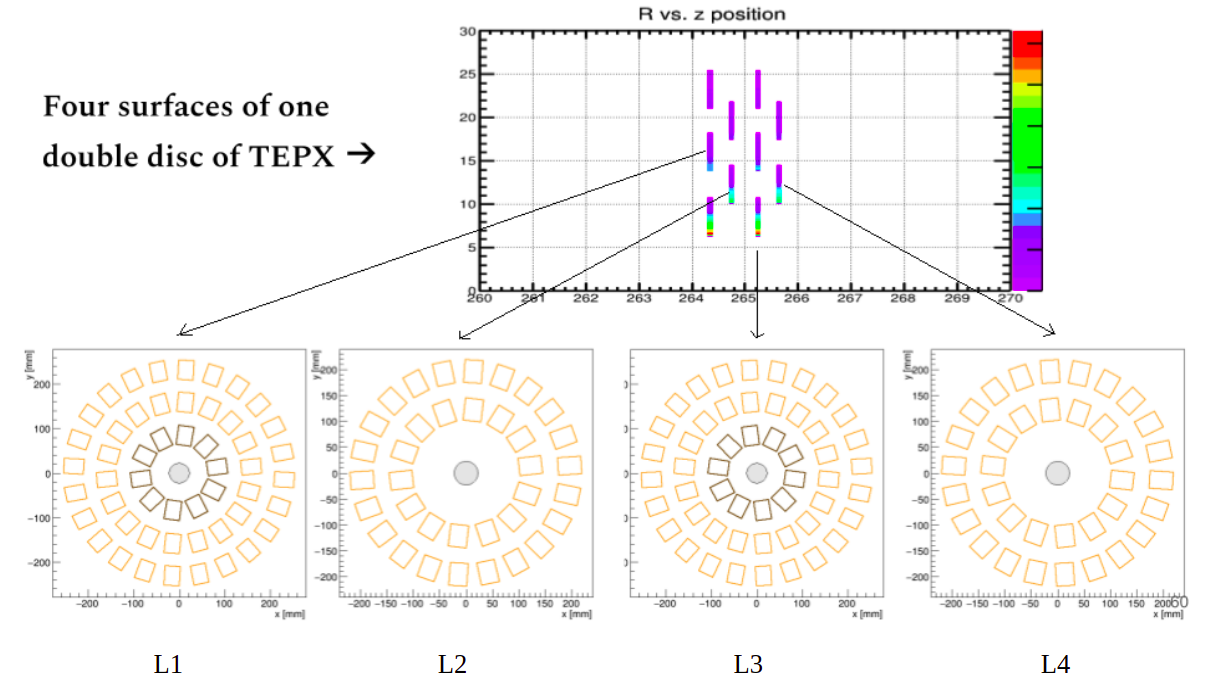
\includegraphics[width=1 \columnwidth]{ashish_thesis/fourlayers.png}
  %\caption[TEPX One Double Disk]{ \onehalfspacing Fours layers of one double disk of TEPX showing module arrangement in rings for each layer. Ring 1, 2, 3, 4 and 5 consists of 20, 28, 36, 44 and 48 modules respectively. }
  %\label{fig:CMS1_49}
%\end{figure}

\section{TEPX Luminomter Simulation}

 Simulated data samples for Phase II include full CMS detector description and uses official CMS software (version $\texttt{CMSSW\_10\_6\_0\_patch2}$) which calls GEANT4 for detector simulation \cite{GEANT4:2002zbu}.  Pixel clusters are reconstructed using the standard CMS reconstruction algorithms \cite{cmssw_2024}. It is done by converting raw data to digi format (row, column, charge) and then form clusters from digis. The samples used in simulation use single-neutrino generated events overlaid with a variable number of minimum-bias events (events with any amount of real energy detected in CMS) to simulate different pileup values.  The number of simulated events used in this analysis for each pileup value is shown in Table \ref{tab:12}.
 
\begin{comment}

\begin{table}[ht]
  \centering
  \caption[Phase II simulated samples]{Total number of events in Phase II CMS tracker simulated samples}
  \begin{tabular}{cc}
    \textbf{pileup} & \textbf{Total number of events} \\
    \hline
    noPU  & 500000 \\
    0.5 & 500000 \\
    1 & 500000 \\
    1.5 & 500000 \\
    2 & 500000 \\
    10 & 100000 \\
    30 & 100000 \\
    50 & 100000 \\
    100 & 100000 \\
    140 & 99600 \\
    200 & 100000 \\
  \end{tabular}
  \label{tab:12}
\end{table}

\end{comment}

%The dataset is a simulated sample designed to evaluate the phase-2 upgrade of the CMS tracker. It includes a range of pileup conditions, from zero to 200 collisions per bunch crossing. Generated using a neutrino gun for events and version 10.6.0 of the CMS Software, the dataset aims to replicate conditions expected for the 2023 CMS upgrade. The data goes through a three-step process that consists of generating initial events, simulating the detector's response, and reconstructing physics objects for further study.
%Table \ref{tab:sample_1} provides information about the number of events per file in relation to  pileup. Pileup is used to denote the number of pp collisions per bunch crossing. In the table, the pileup ranges from 'noPU' (no pileup) to a pileup of 200. As the pileup increases, the number of events per file generally decreases. For example, with no pileup, there are 2000 events per file. At a pileup of 0.5, this remains the same. However, as the pileup increases to 1, the number of events drops to 1800. The decrease continues progressively until a pileup of 2, where there are 1400 events per file. Beyond a pileup of 10, the number of events per file dramatically drops and stays constant at 100 events per file for pileups from 50 to 200. The number of event processed in this study for each pileup is shown in Table \ref{tab:sample_2}.

\begin{comment}

\begin{table}[ht]
  \centering
  \caption{Events per file for each pileup}
  \begin{tabular}{ccc}
     \textbf{Pileup} & \textbf{Events per file} \\
     \hline
     noPU &   2000\\
     0.5 &   2000\\
     1&    1800\\
      1.5&  1500\\
      2&   1400\\
     10&    500\\
     30&    200\\
      50&   100\\
      100&   100\\
     140&    100\\
       200&    100\\
  \end{tabular}
  \label{tab:sample_1}
\end{table}

\end{comment}

\begin{table}[ht]
  \centering
  \caption{Events processed for each pileup}
  \begin{tabular}{ccc}
     \textbf{Pileup} & \textbf{Number of events processed} \\
     \hline
     %noPU & 100000  \\
     0.5 &  100600 \\
     1&    87400\\
      1.5& 74900 \\
      2&  66200 \\
     10&   21800 \\
     30&    10000\\
      50&   5000\\
      100&   5000\\
     140&    5000\\
       200&    5000\\
  \end{tabular}
  %\caption{Events processed for each pileup}
  \label{tab:12}
\end{table}

\begin{comment}

\section{Luminosity measurement using TEPX}

%Luminosity measurement for Phase II HL-LHC pixel detector will be done using two different systems: TEPX and D4R1 \cite{Haranko2023}. TEPX will be used in physics for tracking but will also get a dedicated trigger generated by the BRIL trigger board, data will be only processed by luminosity hardware of TEPX and send to BRILDAQ. D4R1 will be a dedicated luminometer with dedicated triggers fully independent of the CMS DAQ system for data analysis. Luminosity measurement using TEPX will be based on real time pixel cluster/coincidences counting (PCC) on FPGA, a method which involve counting the number of pixel clusters in the pixel detector (innermost part of the CMS tracker) per bunch crossing in minimum bias events. The innermost ring of the last disk of TEPX (D4R1) is located at 2.65 m away from the interaction point that is beyond the tracking acceptance ($|\eta| = 4$) and as this region has few tracking points, it can be solely used for the purpose of luminosity measurement by using the full available trigger rate and bandwidth \cite{Collaboration:2706512}. D4R1 will have dual purpose, luminosity and beam induced background (beam gas & beam halo) measurements. It will be operated during LHC ramp when beams are not colliding for measuring beam induced backgrounds. First bunch in a train or noncolliding bunches will be used for beam-induced background measurements.

During Phase II HL-LHC, the pixel detector's luminosity will be measured using two systems: TEPX and D4R1 \cite{Haranko2023}. TEPX, primarily for tracking in physics, will also have a dedicated BRIL trigger for luminosity data, processed and sent to BRILDAQ. D4R1, a separate luminometer, operates independently of the CMS DAQ system  \cite{Collaboration:2706512}. TEPX's luminosity measurement uses real-time pixel cluster counting (PCC) on FPGA, tracking clusters per bunch crossing in minimum bias events. D4R1, located at 2.65 m from the interaction point and beyond tracking acceptance, focuses on luminosity and beam-induced background measurements, including during non-colliding LHC ramps.

Expected CMS L1 trigger rate is around 750 kHz at pileup 200. 500 kHz trigger rate during van der meer scans (pileup 0.5) and 75 kHz (10\% of expected CMS L1 trigger rate) trigger rate will be used for TEPX luminosity measurement at pileup 200. 1000 kHz trigger rate during van der meer scans (pileup 0.5) and 825 kHz trigger rate will be used for D4R1 luminosity measurement at average pileup 200.

The TEPX and D4R1 detectors will utilize an independent BRIL trigger board (BTB) for luminosity measurement, separate from the CMS L1 trigger system. This setup includes a local control stream synchronized with the LHC clock. Data from TEPX will be transmitted via high-speed links and processed by an FPGA for pixel clustering and histogramming, ensuring synchronization with CMS's overall timing and control system.

\begin{comment}
TEPX and D4R1 will require BRIL trigger board (BTB) independent of CMS L1 trigger system to have full control over luminosity triggers, local TCDS2-like control stream for D4R1 synchronised to LHC clock, luminosity local L1 triggers, encoding of beam 1 & beam 2 logical signals. CMS Timing and Control Distribution System (TCDS) receives LHC Clock and Orbit signals that are generated by the LHC RF system and uses them for generating the CMS Clock and commands. Measurement of beam induced background with D4R1 during the LHC ramp will need to be independent but synchronized to the rest of CMS and the central services like TCDS2 and data acquisition will be implemented using special clocking scheme. Trigger and timing subsystem for D4R1 will receive a dedicated “TCDS2-like” control stream from the BRIL trigger board (BTB) that is based on the LHC clock.

Data accepted by CMS L1 trigger (750 kHz) will be collected by the end column of the pixel chip in TEPX and sent through electrical links (eLinks) at 1.28 Gb/s to LpGBT ASICs for optical transmission.
Backend system DTC will be connected to frontend TEPX electronics via low-power Gigabit Transceiver (LpGBT) optical links.
Optical down-links at 2.5 Gb/s will be used for clock, trigger, commands, and configuration data to the pixel modules.
Optical up-links at 10 Gb/s will carry readout data from L1 accept and monitoring information to the DAQ and control system.
TEPX luminosity processing will be performed by a separate luminosity processor board to which the DTC backend will send data over $~$ 4 x 25 Gb/s optical links.

TEPX luminosity processing FPGA will consist of pixel clustering and histogramming instances.
Clustering firmware will consists of
Stream decoder: It will receives TEPX chip data, separate it from data appended by DTC and decode it.
Quarter core processor: It will be used to identify up to four possible clusters within a quarter core. Two hits form a cluster if they touch horizontally, vertically or diagonally.
Quarter core distributor: The quarter core distributor will check a given quarter core for isolation and decides whether it has to be sent to the row merger or counted internally.
Count accumulator: It will receive final data bit and increment cluster count.

\end{comment}

\end{comment}

Fig. \ref{fig:tepx_cl} shows the location of TEPX clusters in Disk 4 in the XY plane (Z is the direction of the beam) from a simulated sample with a pileup of 200 \cite{dabrowski2020}. %Clusters refer to groups of hits in the pixel detector.
It consists of five concentric rings that are color-coded to indicate the density of clusters within the detector. It is transitioning from blue (low density) to red (high density), with the hottest regions indicating the overlap modules within the rings. The granularity of the histogram is set to 1000 for both axes and a bin size of 0.1 mm, allowing for a detailed visualization of the clusters across the disk.
%The TEPX disk in this map consists of 5 rings which are concentric rings of pixel modules at different radial distances from the beamline.

\begin{figure}[H]
  \centering
  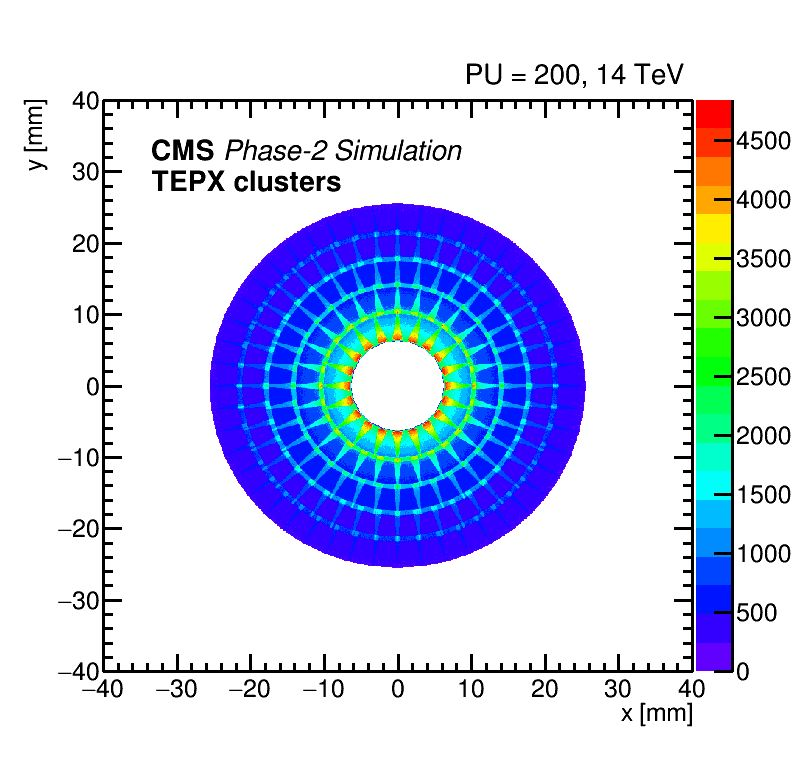
\includegraphics[width=0.7\columnwidth]{ashish_thesis/tepx_clusters_2.png}
  \caption[TEPX Cluster Map]{TEPX cluster map in the XY plane for pileup 200 simulated sample having 5000 events. %Map showing coordinates of TEPX clusters in CMS global coordinate system.
    It shows clusters in one TEPX disk consisting of 5 rings. Hot regions are showing the module overlap. %for all rings (red, orange, green, yellow). Number of x bins is 1000, x bins range from -40 to 40.
    x bin size is 0.1 mm and %Number of y bins is 1000, y bins range from -40 to 40.
    y bin size is 0.1 mm.}
  \label{fig:tepx_cl}
\end{figure}

\begin{figure}[H]
  \centering
  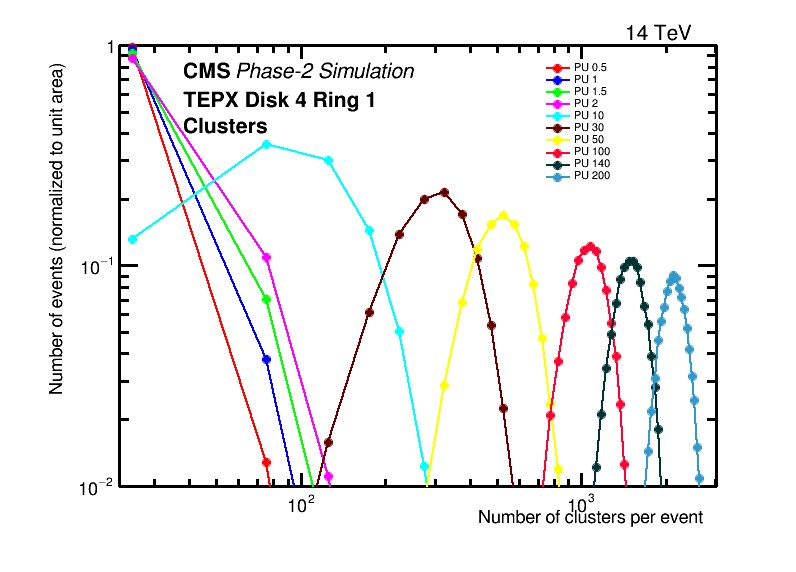
\includegraphics[width=0.7\columnwidth]{ashish_thesis/tepx_D4R!_clusters._allpu_1.png}
  \caption[D4R1 Clusters All Pileup]{Distribution of number of clusters for TEPX Disk 4 Ring 1 for all pileup samples.}
  \label{fig:tepx_cl_allPU}
\end{figure}

\subsection{Linearity of TEPX clusters}

Linearity is one of the systematic uncertainty in the calculation of instantaneous luminosity and PCC visible cross section $\sigma_{vis}$. A linear relation between the mean number of clusters and pileup (PU) imply that $<N_{cl/pp}> = \frac{<N_{cl}>}{\mu} = \frac{\sigma_{vis}}{\sigma_{pp}}$ , $<N_{cl}> =  \frac{\sigma_{vis}}{\sigma_{pp}} \mu $. Linearity indicates that the PCC visible cross section $\sigma_{vis}$ does not depend on the per bunch instantaneous luminosity (ideal luminometer). In ideal scenario, $\sigma_{vis}$ is not dependent on pileup, but this a potential problem with the luminometer. A non-linear relation $<N_{cluster}> = \alpha (PU)^{\gamma}, \gamma \neq 1$ would add non-linear terms in the rate equation $R = \sigma_{vis} L_{inst}$ and cause $\sigma_{vis}$ to vary with the per bunch instantaneous luminosity and pileup values. TEPX luminometer proposed for Phase II shows excellent linearity over entire pileup range.

The number of clusters per pp collision in Disk 4 Ring 1 varies from 0 to 2600 as a function of pileup. At pileup 200, mean number of cluster per pp collision is 2200 as shown in Fig. \ref{fig:tepx_cl_allPU}.
%The peak of the distribution drops as pileup increases because we have processed different number of events for different pileup values. Under low pileup conditions which is crucial for vdM calibration, number of clusters varies from 0 to 35.For average pileup value of 0.5 (vdM conditions), number of clusters varies between 0 and 12.
The distributions follow Poisson statistics. Linearity results for simulated TEPX clusters from low to high pileup values are shown in  Fig. \ref{fig:CMS_4205} and \ref{fig:CMS_4206}. Non-linearity is within 1 \% for entire pileup range.

%\begin{figure}[!htp]
 % \centering
  %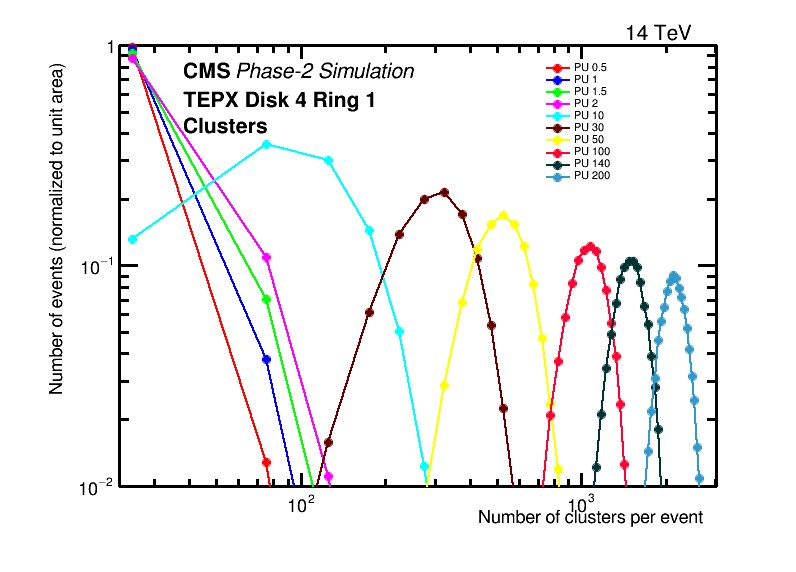
\includegraphics[width=0.6\columnwidth]{ashish_thesis/tepx_D4R!_clusters._allpu_1.png}
  %\caption[D4R1 Clusters All Pileup]{Distribution of number of clusters for TEPX Disk 4 Ring 1 for all pileup values.}
  %\label{fig:tepx_cl_allPU}
%\end{figure}


\begin{figure}[H]
  \centering
  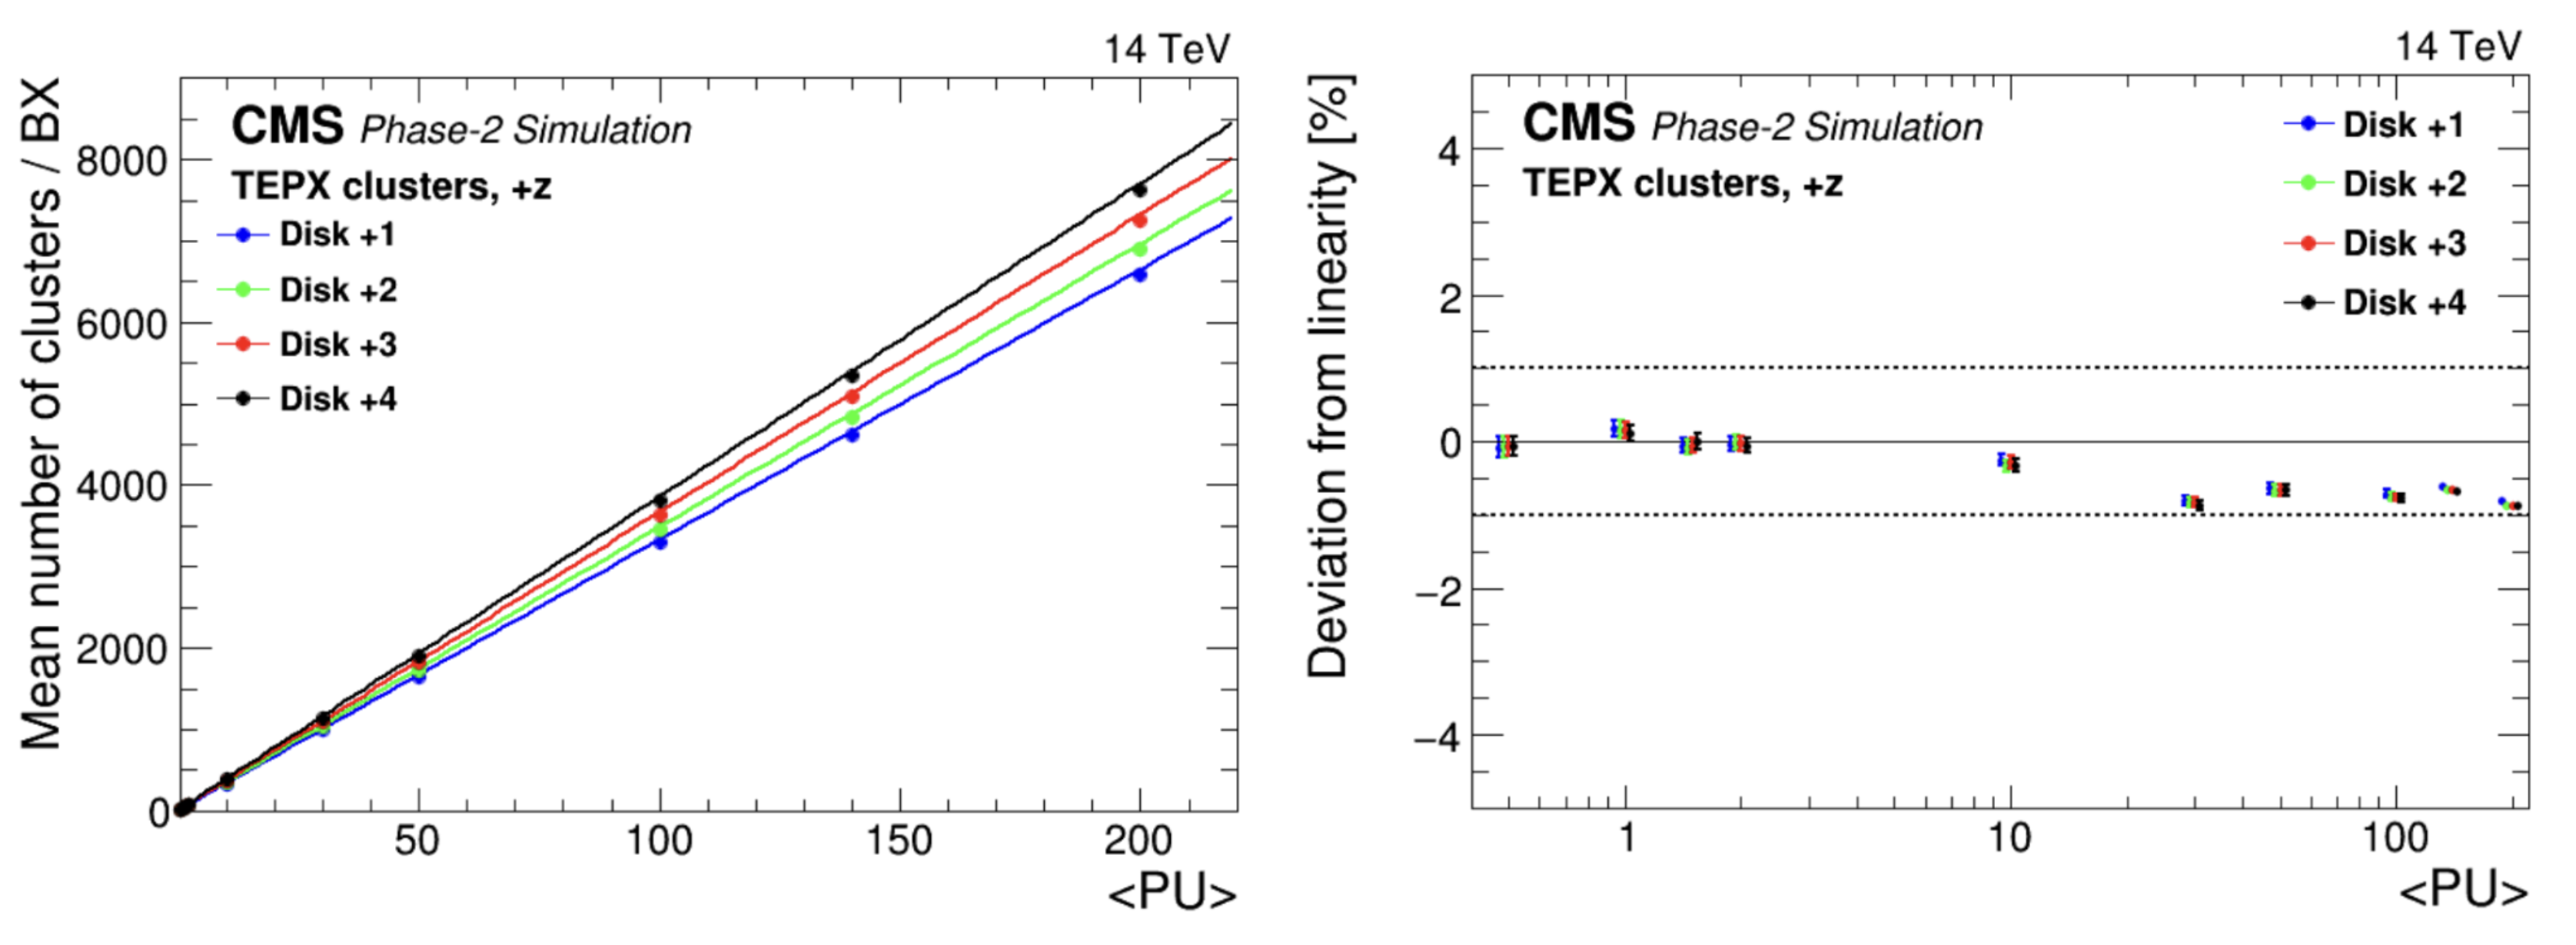
\includegraphics[width=1\columnwidth]{ashish_thesis/michigan_2.png}
  \caption[TEPX cluster linear fit per disk]{\onehalfspacing Left: Simulated mean number of clusters for TEPX disks as a function of pileup. A line is fitted between pileup values of 0 and 2, and then extrapolated up to a pileup of 200. Right: %Deviation from linearity for clusters for  TEPX disks. The non-linearity is calculated as
    The relative difference between the data points and the values of the fit function at the respective pileup value. }
  \label{fig:CMS_4205}
\end{figure}


\begin{figure}[H]
  \centering
  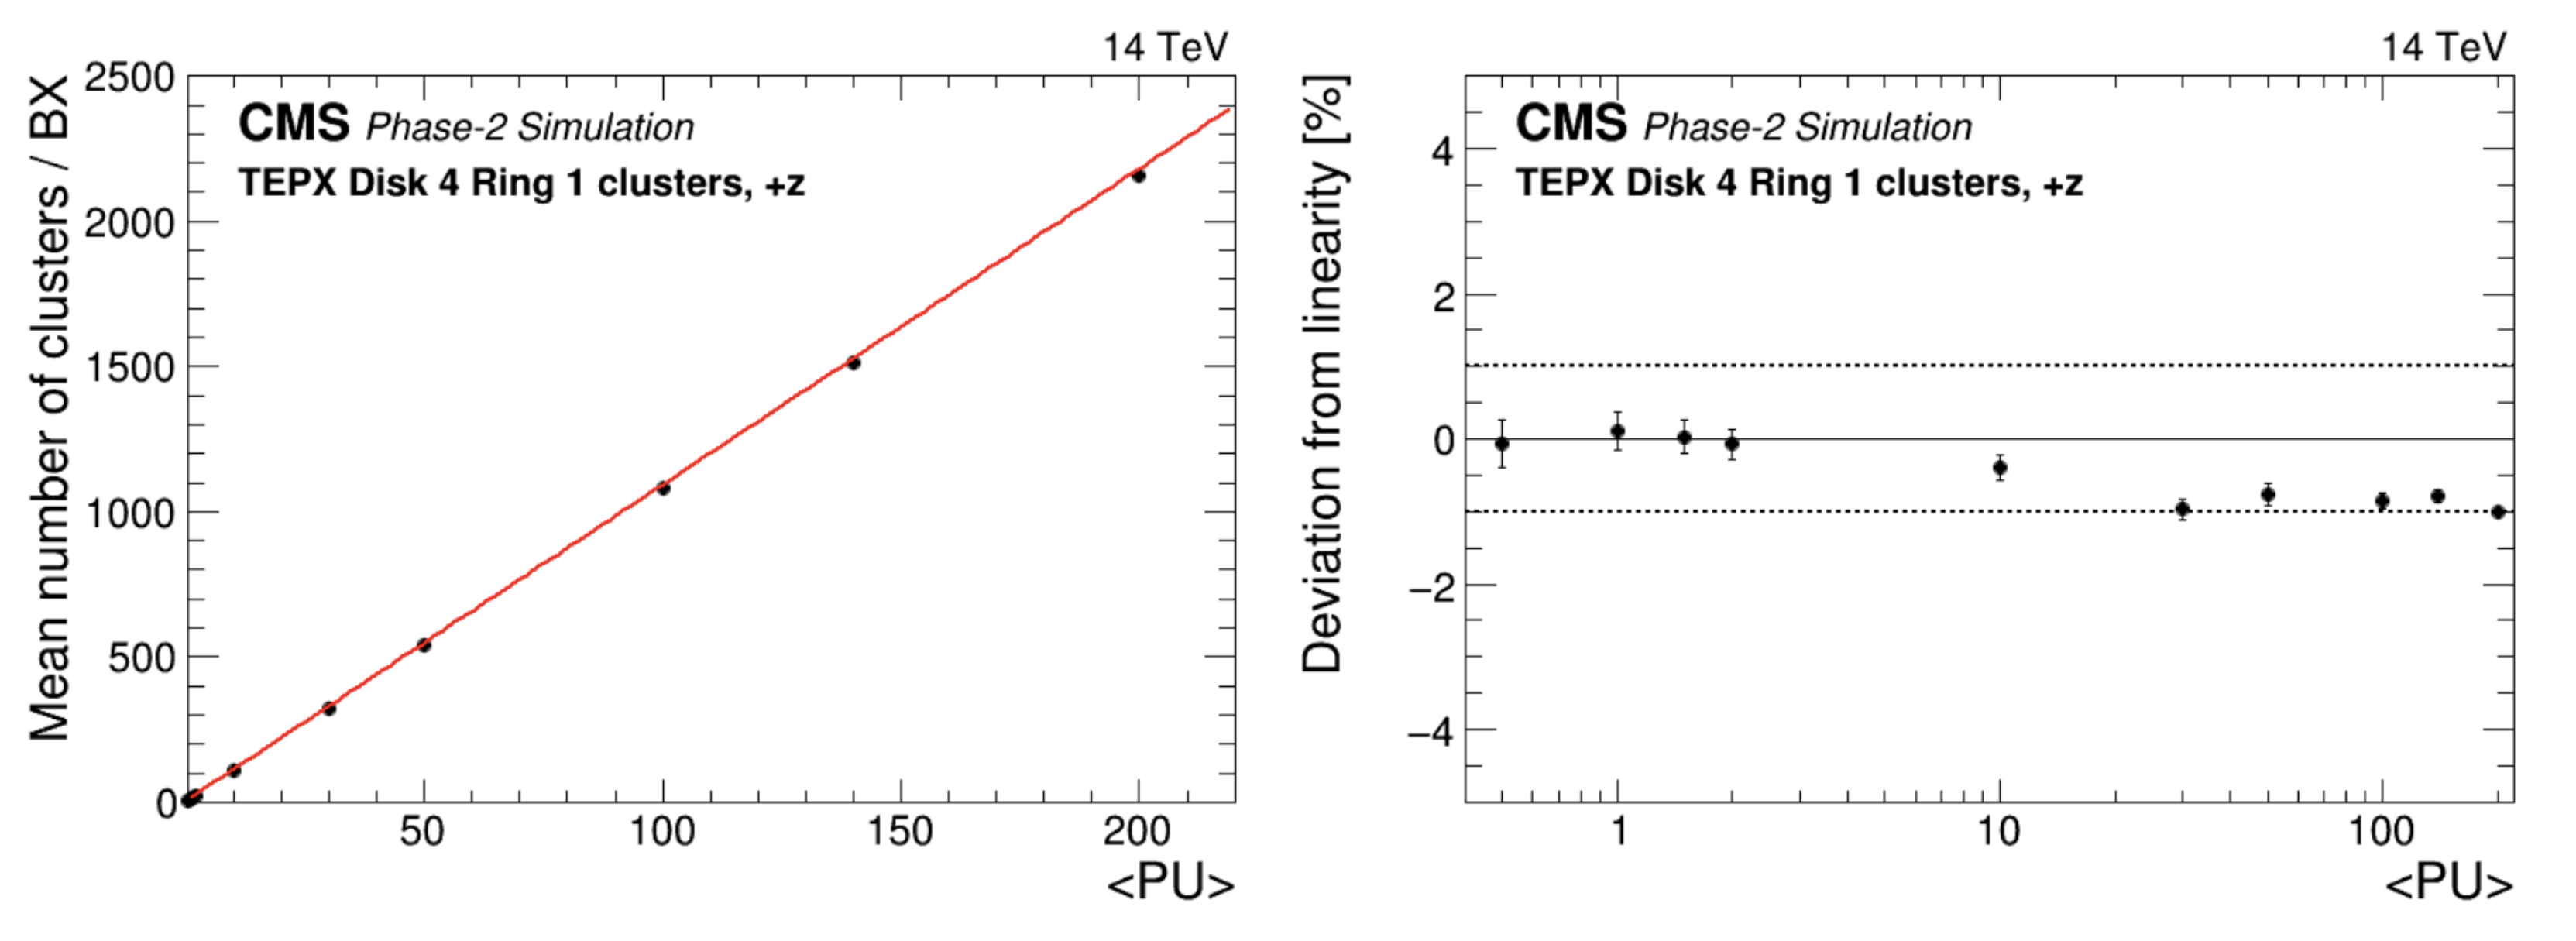
\includegraphics[width=1\columnwidth]{ashish_thesis/michigan_3.png}
  \caption[TEPX clusters linear fit]{\onehalfspacing Left: Simulated mean number of clusters for  TEPX Disk 4 Ring 1 as a function of pileup. A line is fitted between pileup values of 0 and 2, and then extrapolated up to a pileup of 200. Right: %Deviation from linearity for clusters for TEPX Disk 4 Ring 1. The non-linearity is calculated as
    The relative difference between the data points and the values of the fit function at the respective pileup value. }
  \label{fig:CMS_4206}
\end{figure}



\begin{comment}

\begin{figure}[H]
  \centering
  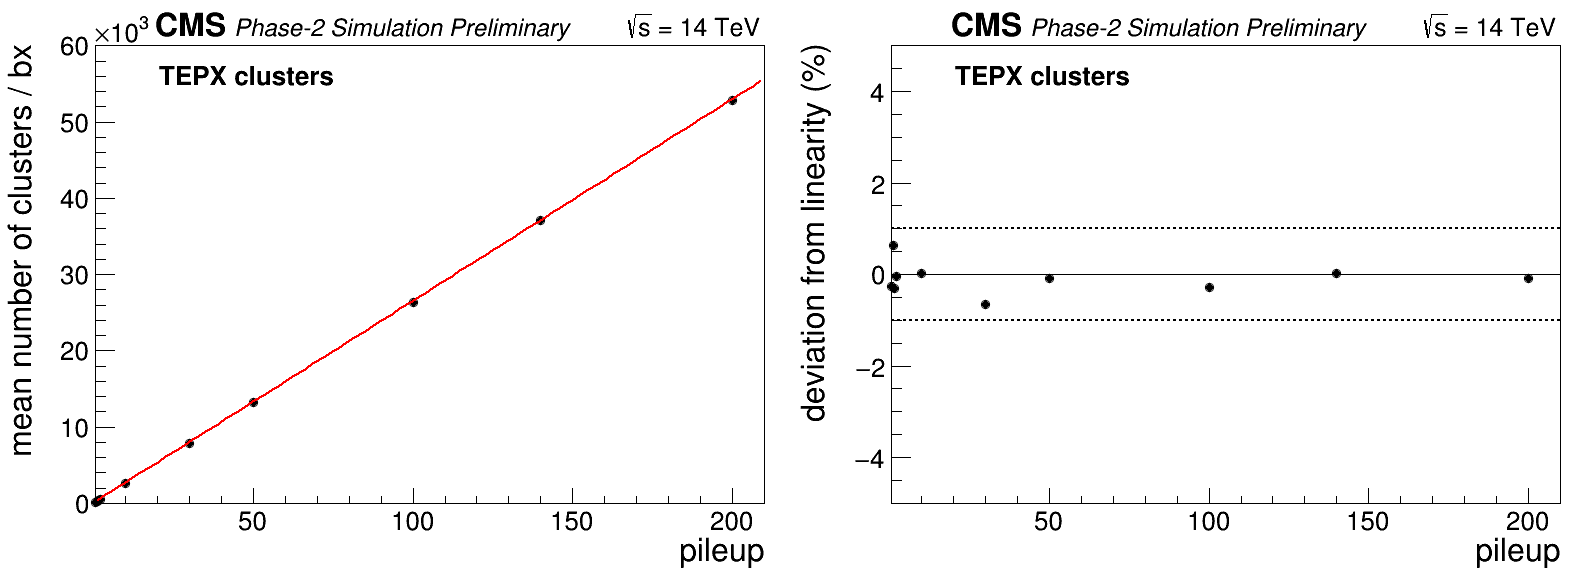
\includegraphics[width=1\columnwidth]{ashish_thesis/totalclusters.png}
  \caption[TEPX Clusters Fit And Residuals]{\onehalfspacing Left: Simulated mean number of clusters for all entire TEPX detector as a function of pileup. A line is fitted between pileup values of 0 and 2, and then extrapolated up to a pileup of 200. Right: Deviation from linearity for clusters for entire TEPX detector. The non-linearity is calculated as the relative difference between the data points and the values of the fit function at the respective pileup value. Non-linearity is within 1 \% for entire pileup range. Pileup 200 corresponds to High Luminosity (HL)-LHC environment.}
  \label{fig:CMS_420}
\end{figure}


\begin{figure}[H]
  \centering
  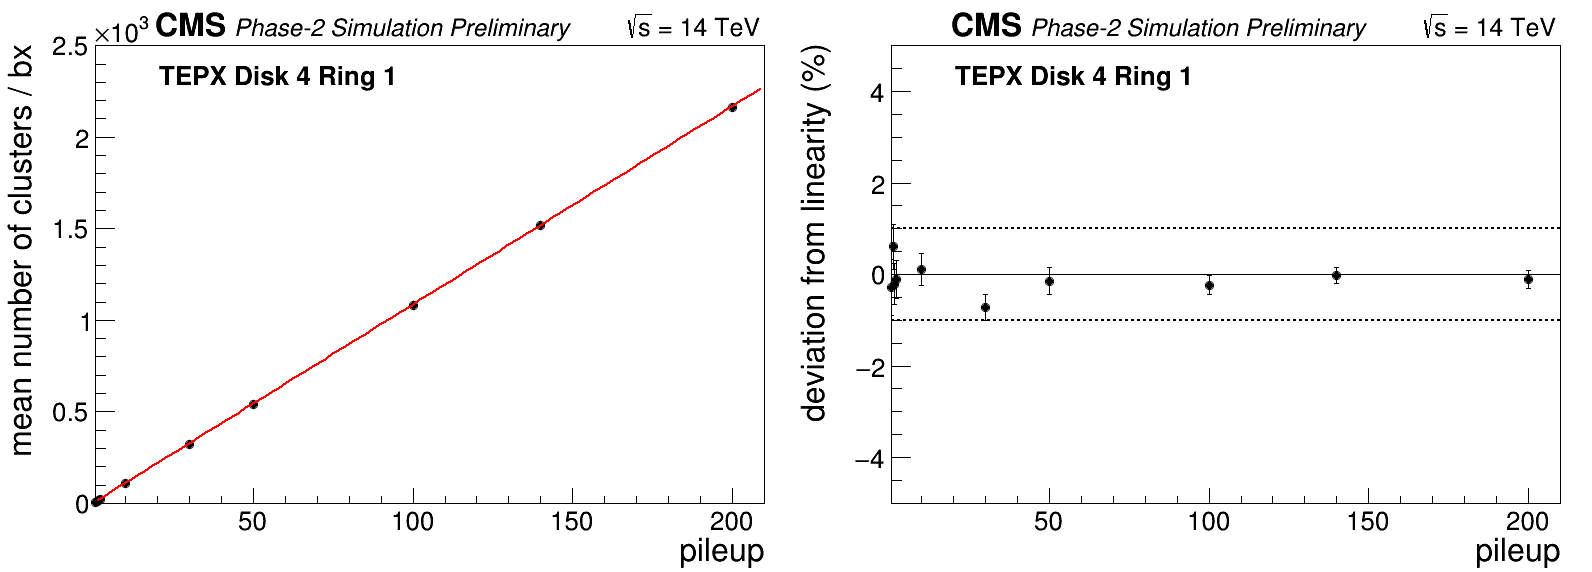
\includegraphics[width=1\columnwidth]{ashish_thesis/clustersD4R1.png}
  \caption[Disk 4 Ring 1 Clusters Fit And Residual]{\onehalfspacing Left: Simulated mean number of clusters for TEPX Disk 4 Ring 1 as a function of pileup. Right: Deviation from linearity for clusters for TEPX Disk 4 Ring 1. The non-linearity is calculated as the relative difference between the data points and the values of the fit function at the respective pileup value.}
  \label{fig:CMS_003}
\end{figure}



\begin{figure}[H]
  \centering
  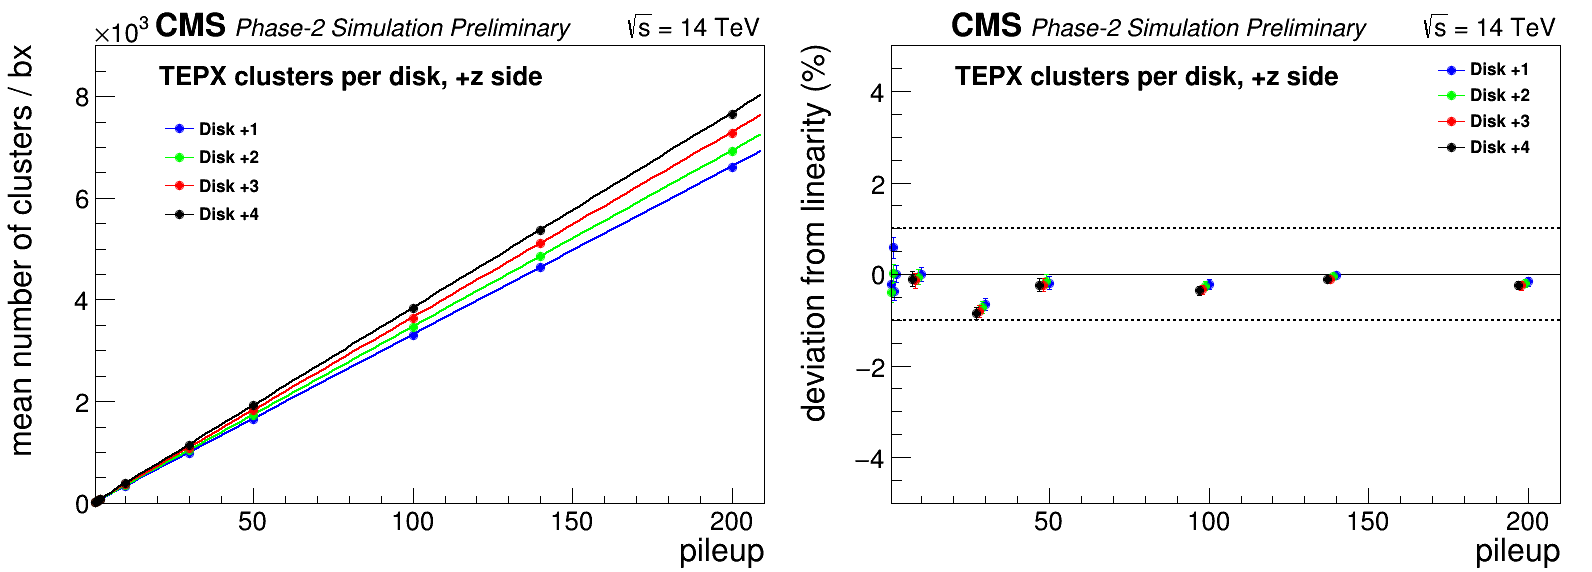
\includegraphics[width=1 \columnwidth]{ashish_thesis/clustersperdisk+z.png}
  \caption[Clusters Per disk Fit And Residual]{Left: Simulated mean number of clusters for +z side TEPX disks as a function of pileup. Right: Deviation from linearity for clusters for +z side TEPX disks.}
  \label{fig:CMS_004}
\end{figure}


\begin{figure}[H]
  \centering
  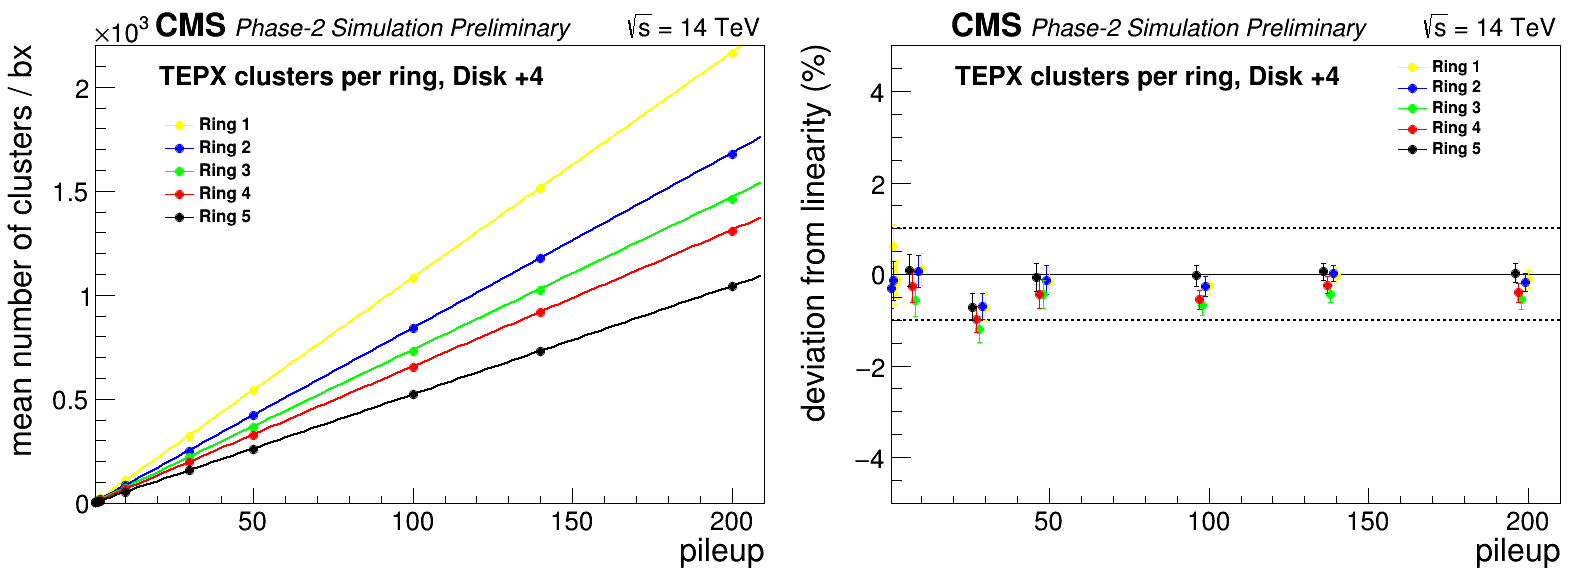
\includegraphics[width=1\columnwidth]{ashish_thesis/clustersperringD+4.png}
  \caption[Clusters Per Ring For Disk 4 Fit And Residual]{Left: Simulated mean number of clusters for +z side TEPX Disk 4 all rings as a function of pileup. Ring 1 has highest slope and Ring 5 has least slope. Right: Deviation from linearity for clusters for TEPX Disk +4 all rings. Non-linearity is within $1\%$ for all rings over entire pileup range.}
  \label{fig:CMS_005}
\end{figure}


\end{comment}


\subsection{TEPX two-fold coincidences}

Two-fold coincidences are clusters in modules overlap regions formed by modules in front layers (L1-L3) and back layers (L2-L4) separately. There are two types of two-fold coincidences namely in $\phi$ and r. Two-fold coincidence in $\phi$ involve modules overlap in the same ring of one double-disk and two-fold coincidence in r require modules overlap between successive rings of one double-disk.  Two-fold coincidences are better way to distinguish between a real hit and random noise. %They are more likely to be real hit than random electrical noise.
Luminosity determination based on counting coincidences has an advantage over clusters that afterglow effects are tiny. %in the case of coincidences. 
%as shown in Fig. \ref{fig:cluster_ring_4000}. 
 %(shown in Fig. \ref{fig:cluster_ring_73})
  %as depicted in Fig. \ref{fig:cluster_ring_74}. 
 %Overlap between L1 L3 and L2 L4 layers also possible but we havent considered them in this simulation. L1L2 two fold coincidences in r are clusters in module overlaps between adjacent rings in first two layers. L3L4 two fold coincidences in r are modules overlaps in the last two layers between adjacent rings. All types of two fold coincidences in r are shown in Table \ref{tab:twofoldinr}. Module overlap between different rings for all types of two fold coincidences in r are shown in Fig. \ref{tab:twofoldinr}. Two fold coincidences are better way to distinguish between a real hit and random electrical noise. They are more likely to be real hit than random electrical noise. Luminosity determination based on counting coincidences has an advantage over clusters that afterglow effects are tiny in the case of coincidences.

\begin{comment}

\begin{figure}[!htp]
\centering
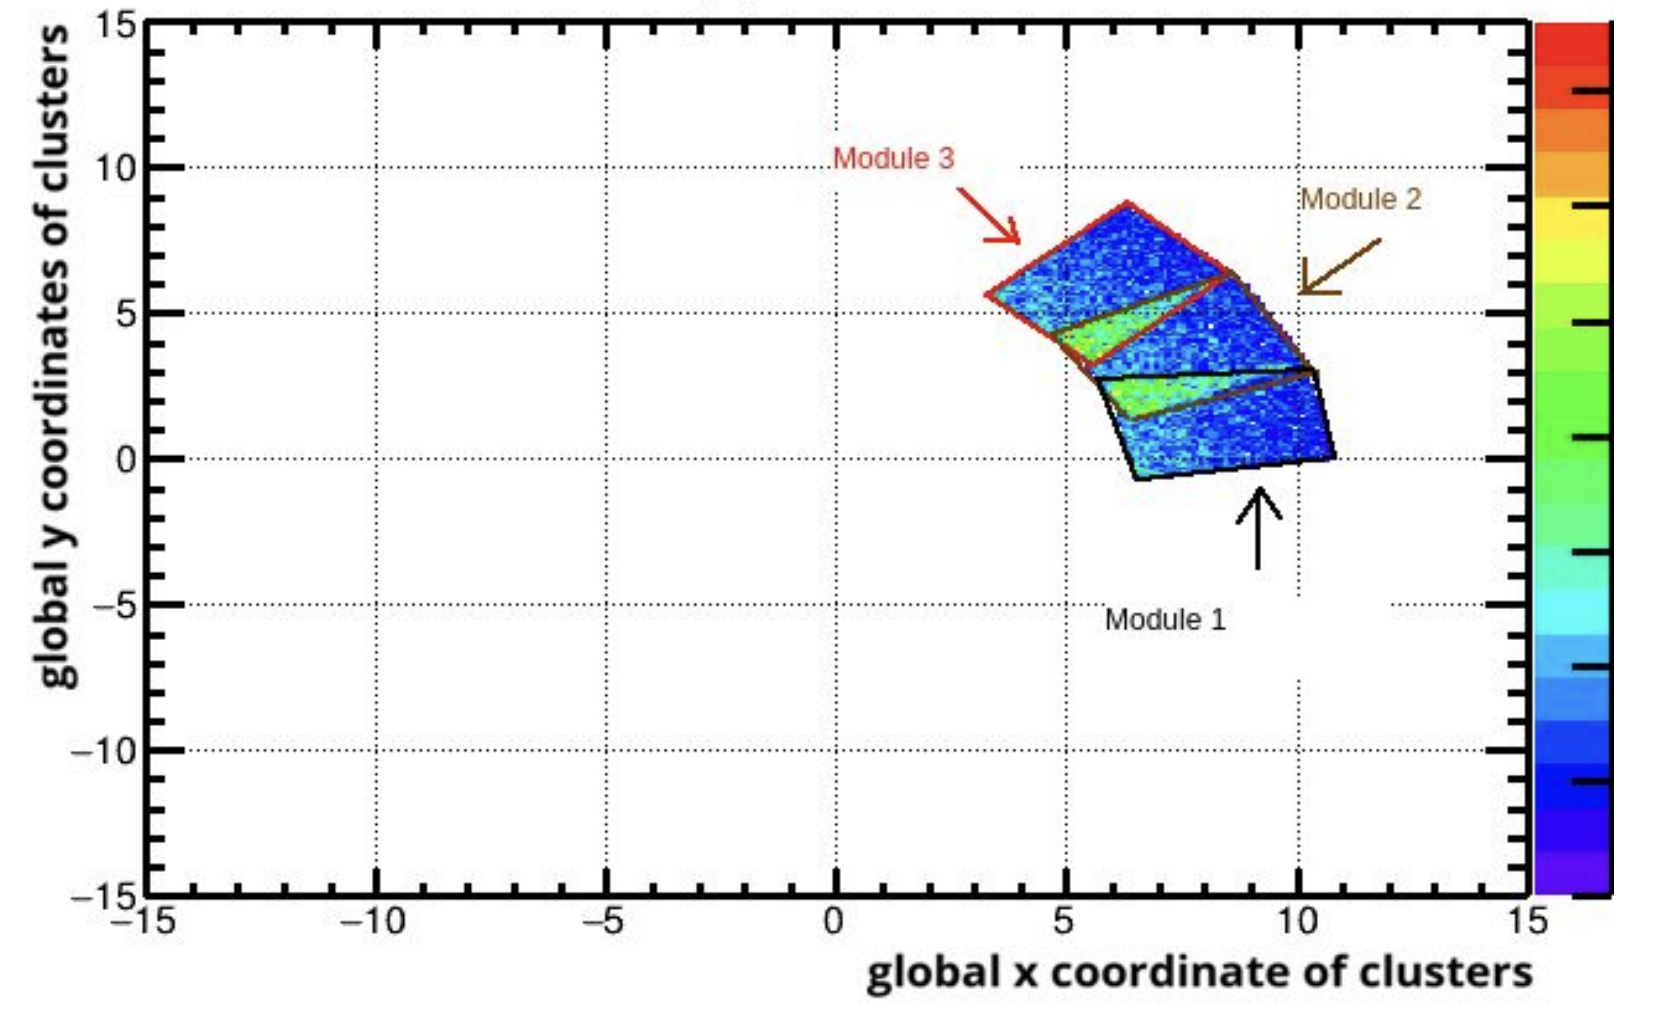
\includegraphics[width=0.6\textwidth]{ashish_thesis/twofoldinphi.png}
\caption[Module Overlap Two Fold Coincidences in phi]{%                                                                                                                                     
  Example of module overlap between same ring modules that can give rise to two fold coincidences in phi.
}
\label{fig:cluster_ring_4000}
\end{figure}

\begin{table}[ht]
  \centering
  \caption{Location of four layers in Disk 4}
\begin{tabular}{cc}
\textbf{Layer} & \textbf{z coordinate} \\ 
\hline
Layer 1 (L1) & 264.4 \\ 
Layer 2 (L2) & 264.8 \\ 
Layer 3 (L3) & 265.2 \\ 
Layer 4 (L4) & 265.6 \\ 
\end{tabular}
\label{tab:alllayerz}
\end{table}

\begin{table}[ht]
  \centering
  \caption{Types of two fold coincidences in r}
\begin{tabular}{ccc}
\textbf{Type of two fold coincidences in r} & \textbf{Module overlap} & \textbf{dz} \\ 
\hline
A & R1L1-R2L2 & 0.4 \\ 
B & R1L1-R2L4 & 1.2 \\ 
C & R1L3-R2L4 & 0.4 \\ 
D & R2L2-R3L3 & 0.4 \\
E & R3L1-R2L2 & 0.4 \\ 
F & R3L3-R2L4 & 0.4 \\ 
G & R3L1-R4L2 & 0.4 \\ 
H & R3L1-R4L4 & 1.2 \\ 
I & R3L3-R4L4 & 0.4 \\ 
J & R5L1-R4L2 & 0.4 \\ 
K & R4L2-R5L3 & 0.4 \\ 
L & R5L3-R4L4 & 0.4 \\ 
\end{tabular}
\label{tab:twofoldinr}
\end{table}

\begin{figure}[!htp]
\centering
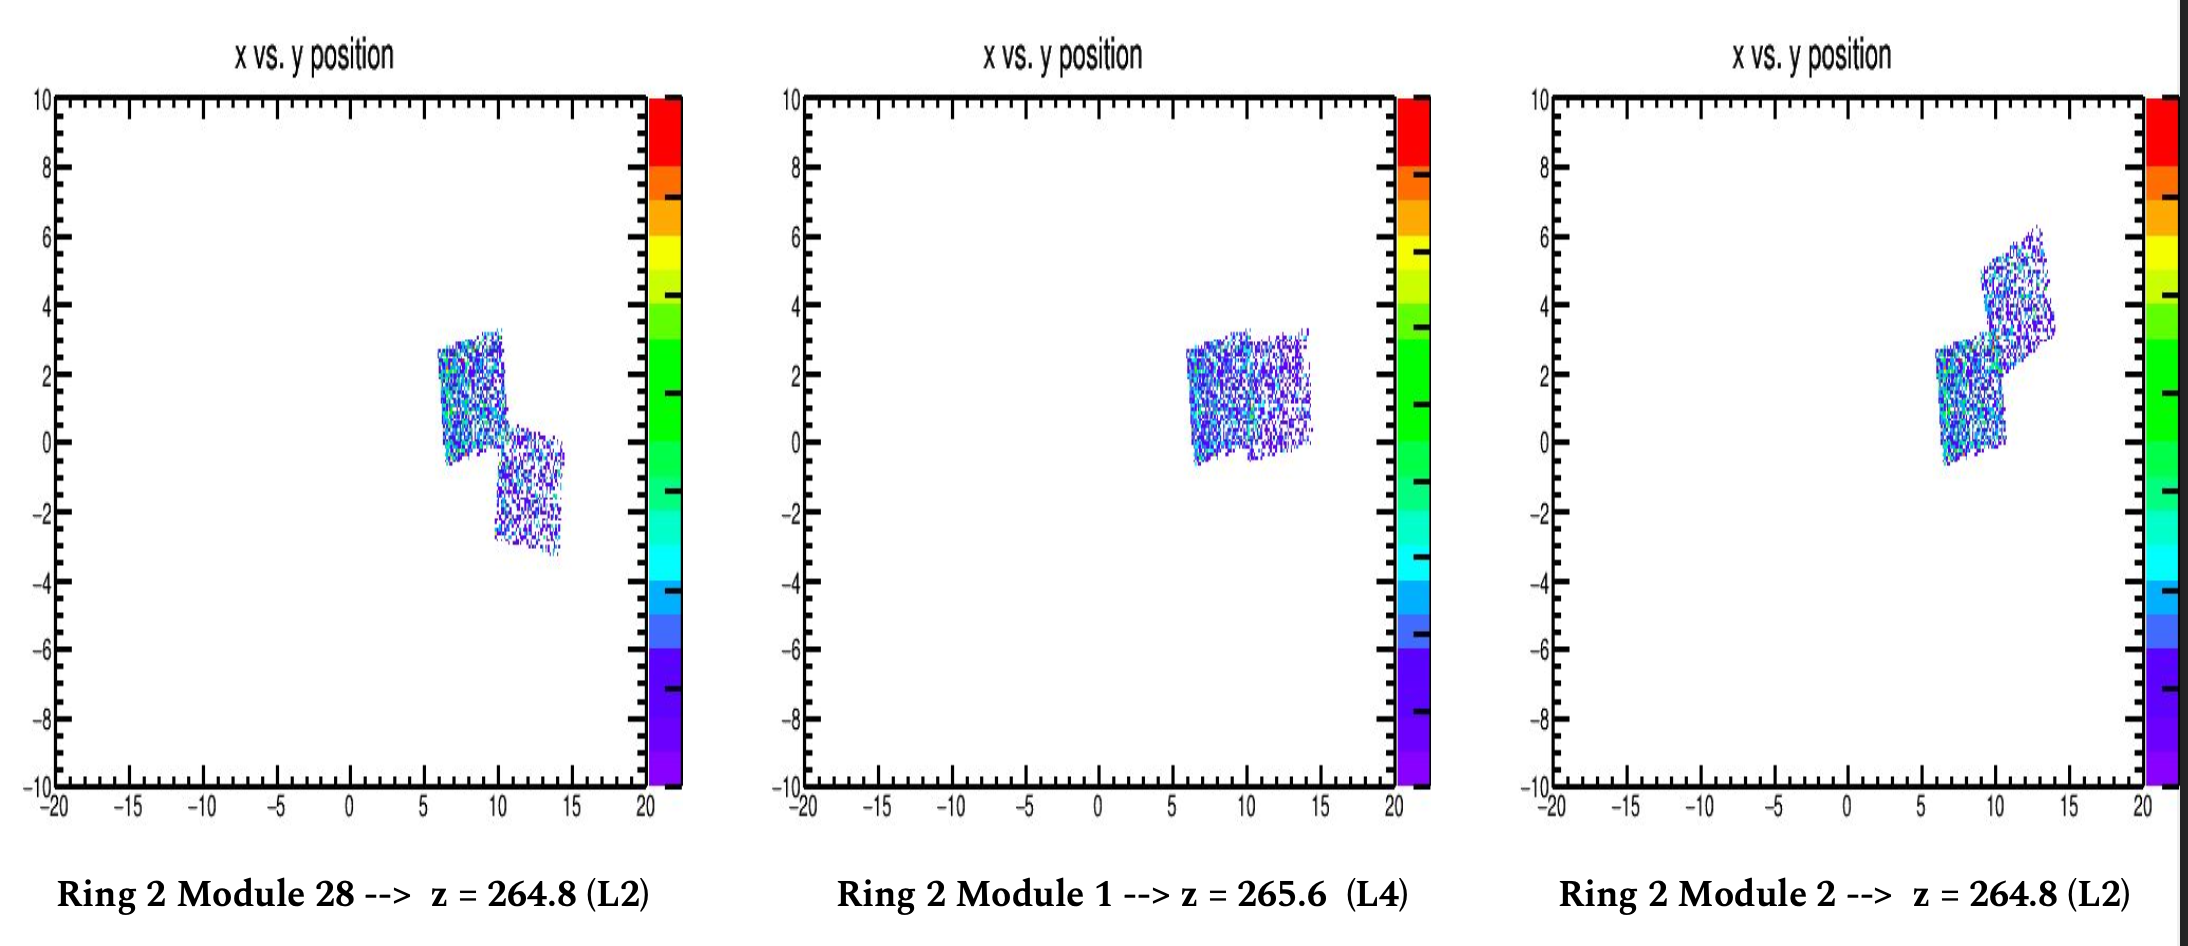
\includegraphics[width=1\textwidth]{ashish_thesis/moduleoverlapinR_1.png}
\caption[Module Overlap Two Fold Coincidences in r]{%                                                                                                                                                                         
  Example of module overlap between different ring modules that can give rise to two fold coincidences in r.
}
\label{fig:cluster_ring_73}
\end{figure}

\begin{figure}[!htp]
\centering
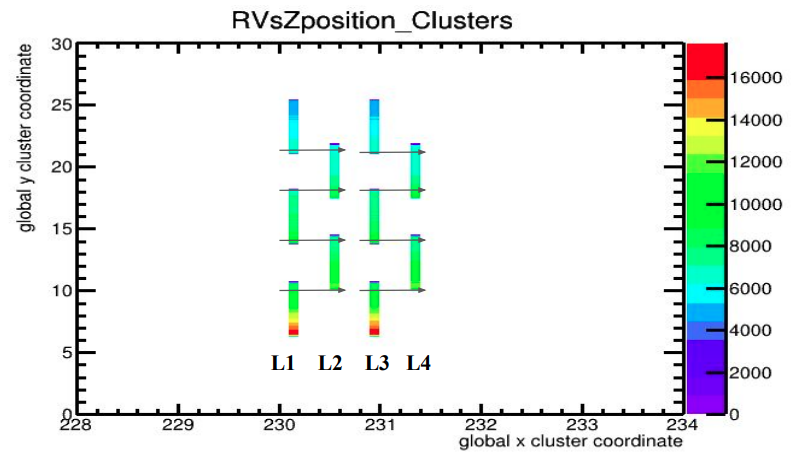
\includegraphics[width=1\textwidth]{ashish_thesis/twofoldinRmethod.png}
\caption[Few types Of Two Fold Coincidences in r]{%                                                                                                                                                                              
  Example of module overlap between different ring modules in the first two and last two layers of one tepx double disk that can give rise to two fold coincidences in r.
}
\label{fig:cluster_ring_74}
\end{figure}

\end{comment}


%\begin{figure}[!htp]
 % \centering
  %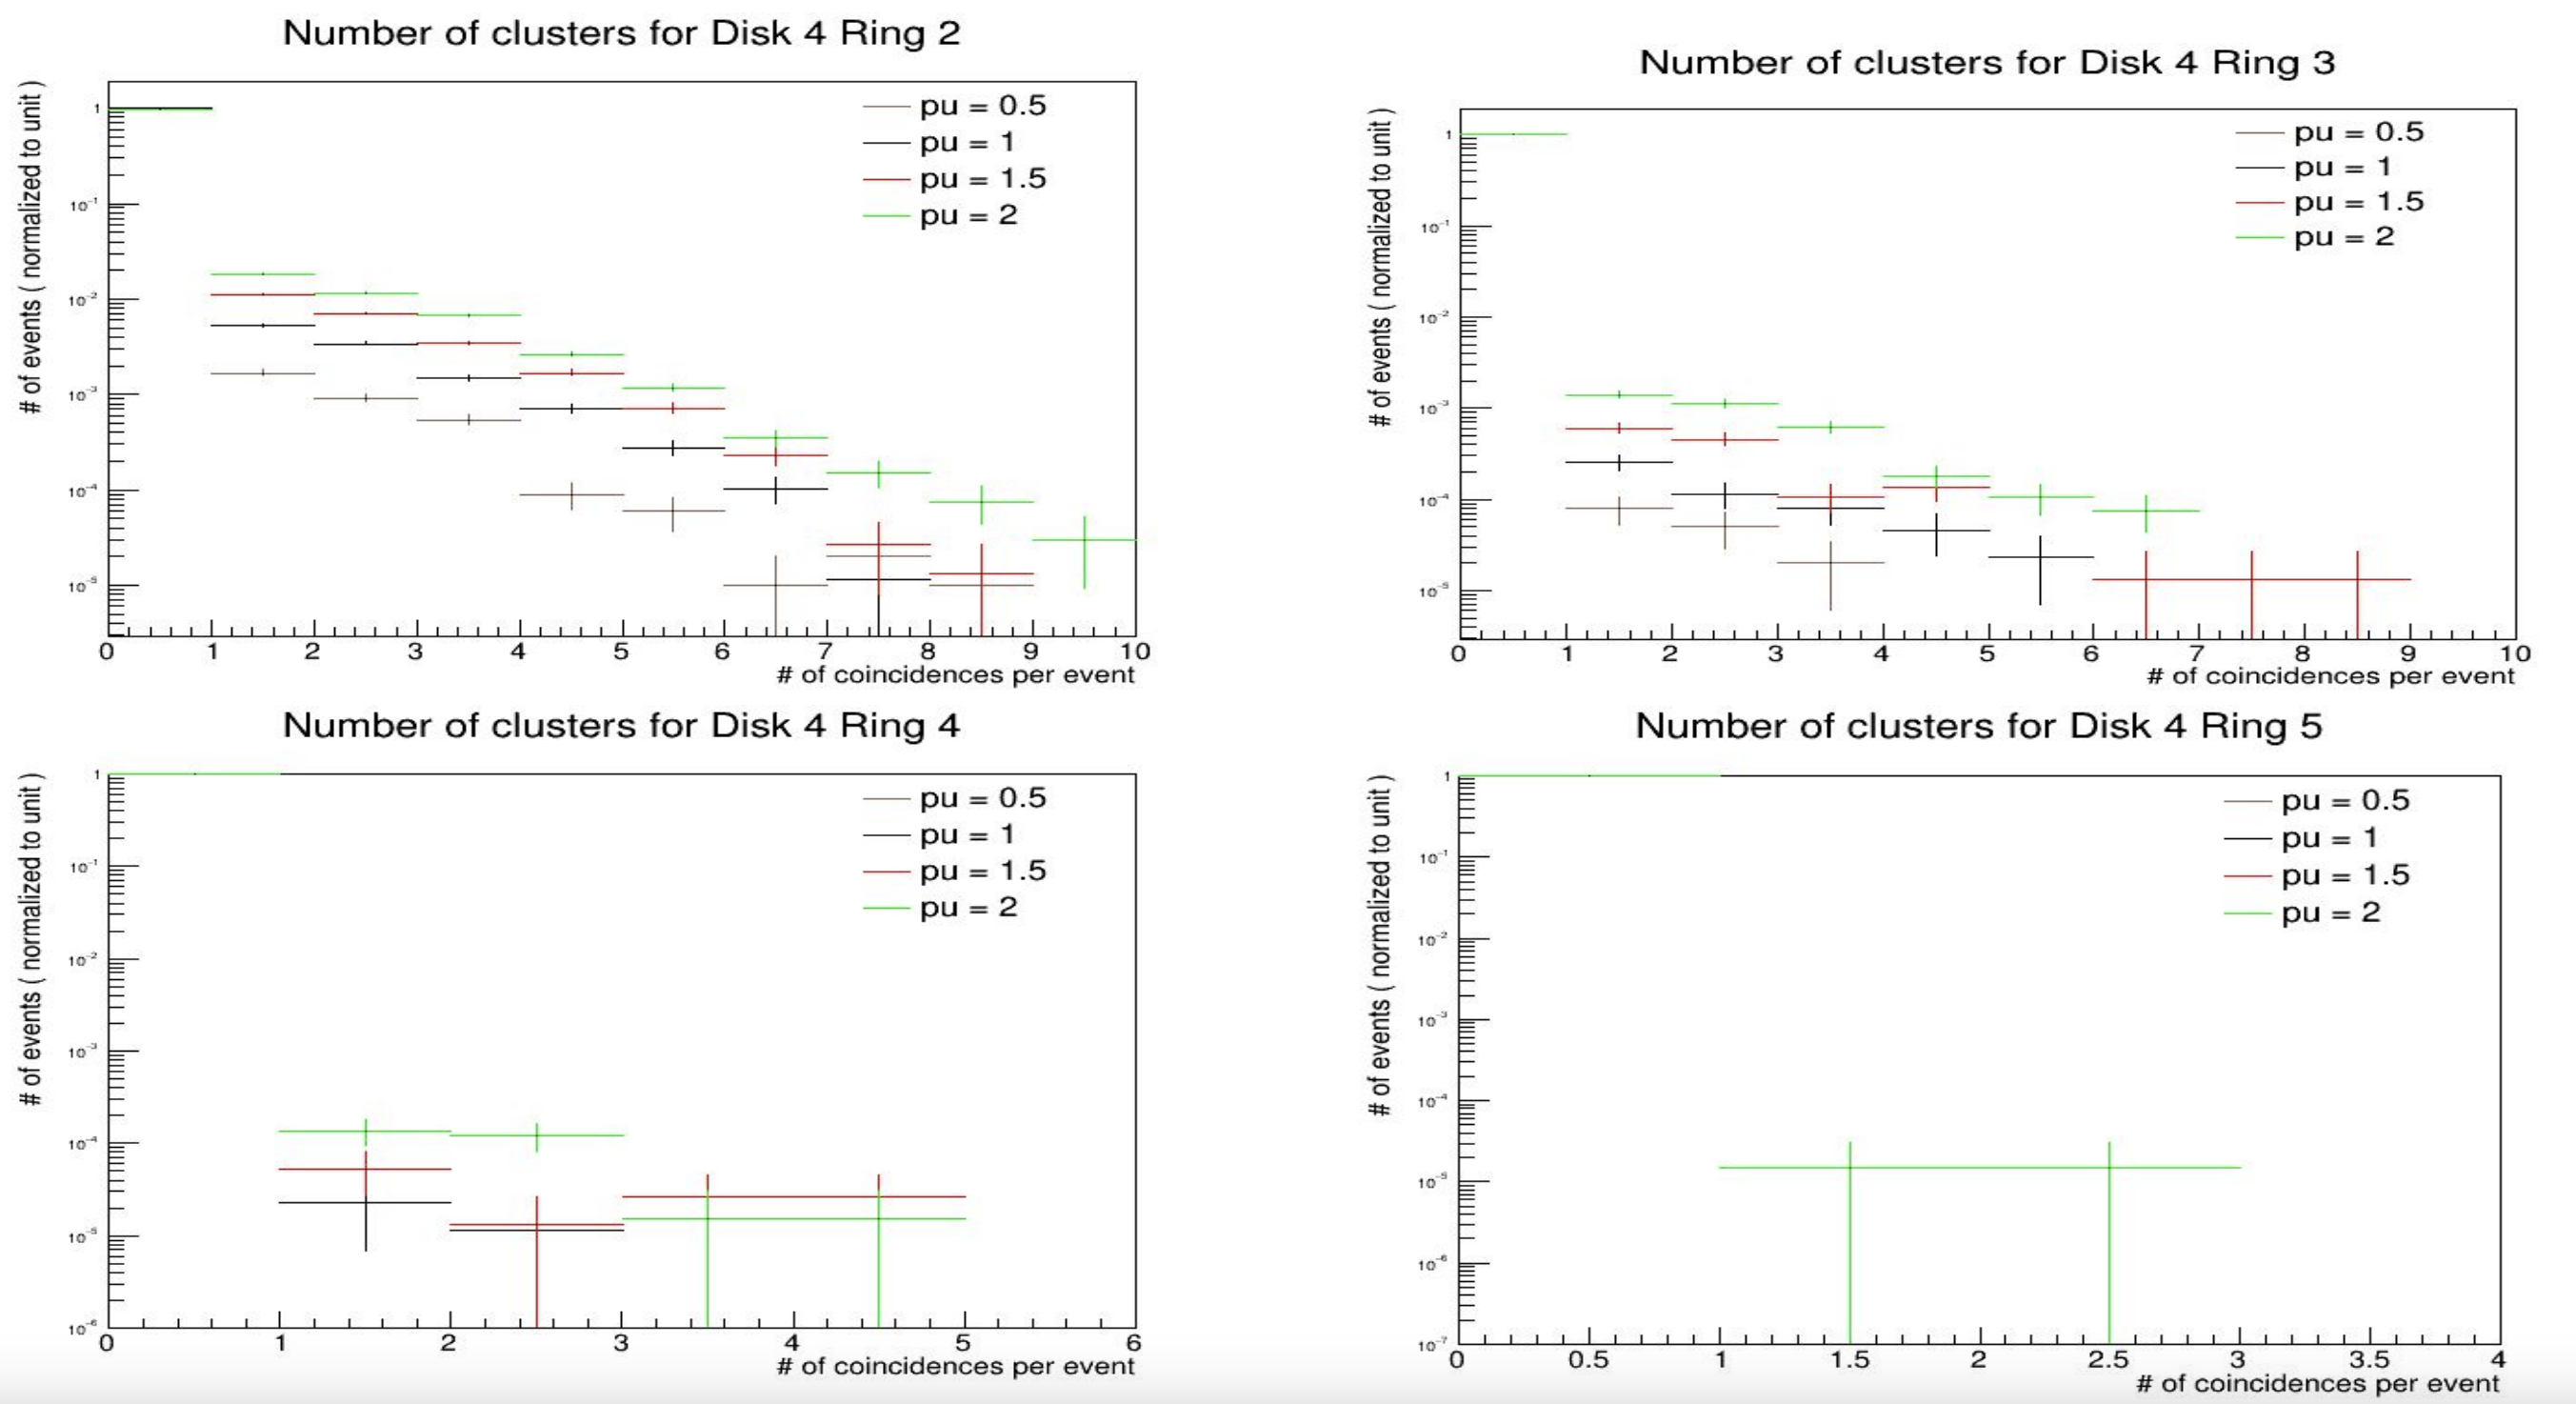
\includegraphics[width=1\columnwidth]{ashish_thesis/tepx_D4_3foldcoin_lowpu.png}
  %\caption[TEPX D4 All Rings Three Fold Coincidences Low Pileup]{Distribution of number of three fold coincidences for TEPX Disk 4 all rings for low pileup values.}
  %\label{fig:tepx_3foldcoin_lowPU}
%\end{figure}

\begin{comment}

The old algorithm for defining two fold coincidence employ x and y global position coordinates of clusters \cite{dabrowski2020}. Separation between x and y coordinate of original and coincidence cluster with proper selection and z coordinate selection in accordance with the separation between different layers in tepx disk is used as shown in Fig. \ref{fig:oldvar_xy}.

dx=x2-x1, dy=y2-y1

\begin{itemize}

\item Two fold coincidence in this algorithm is defined as the pair of hits in the module overlap region within TEPX disk satisfying dx and dy selections of 0.1 and separated by z coordinate of 0.9.

\item True coincidences are hits in module overlap region satisfying dx, dy selections of 0.1 and generated by same simulated track id.

\item Fake coincidences are hits in module overlap region satisfying same dx, dy selections of 0.1 but not generated by same simulated track id.

\end{itemize}

\begin{figure}[!htp]
\centering
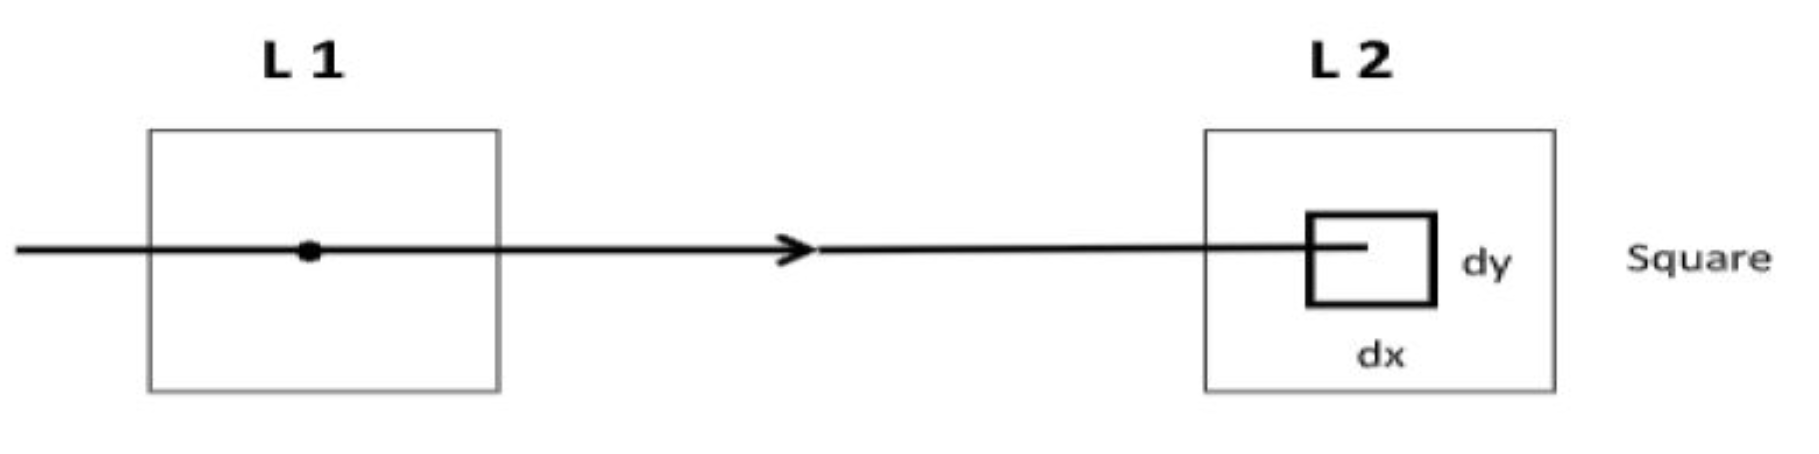
\includegraphics[width=1\textwidth]{ashish_thesis/oldvariable_xy.png}
\caption[Old Definition Of Two Fold Coincidences]{%
   Old x, y variables used for defining two fold coincidences clusters in phi.
}
\label{fig:oldvar_xy}
\end{figure}


\begin{figure}[!htp]
\centering
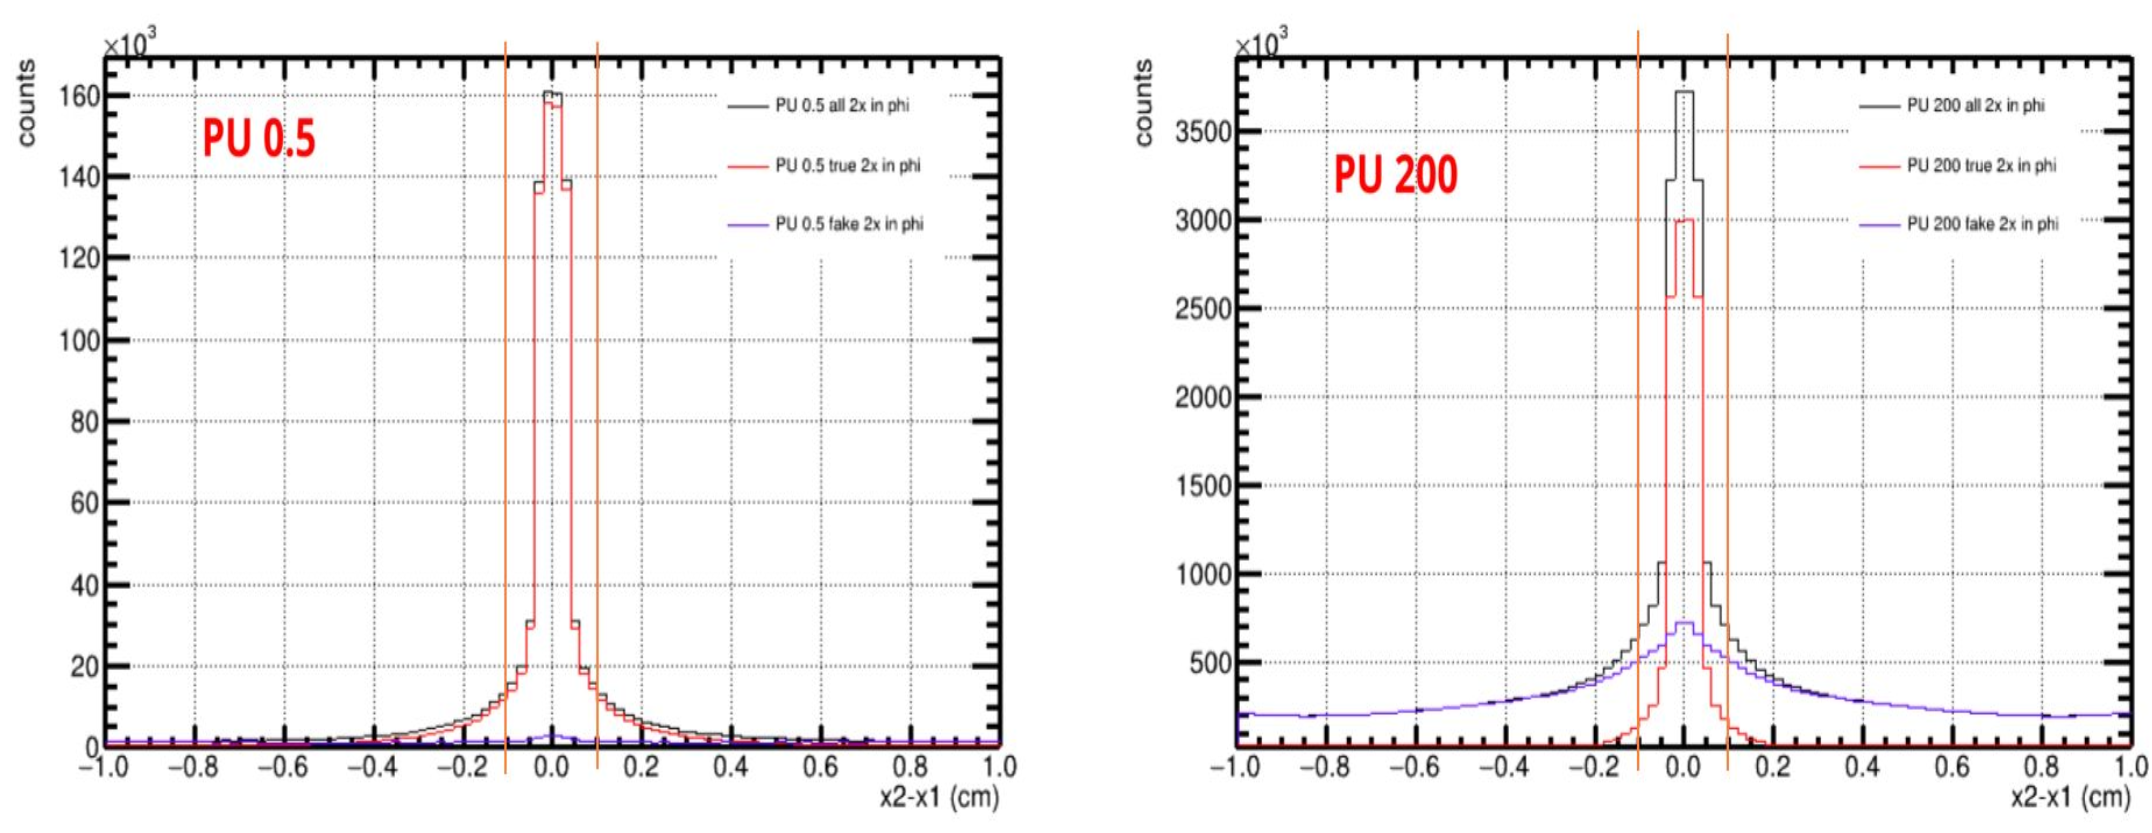
\includegraphics[width=1\textwidth]{ashish_thesis/twofoldcoin_inphi_PU0p5_200.png}
\caption[Total, True and Fake Two Fold coincidences in phi (old x variables)]{%
 Separation between x coordinates of clusters in module overlap region for pileup 0.5 and 200 showing distribution total, true and fake two fold coincidences in phi.
}
\label{fig:dx_twofold}
\end{figure}


\begin{figure}[!htp]
\centering
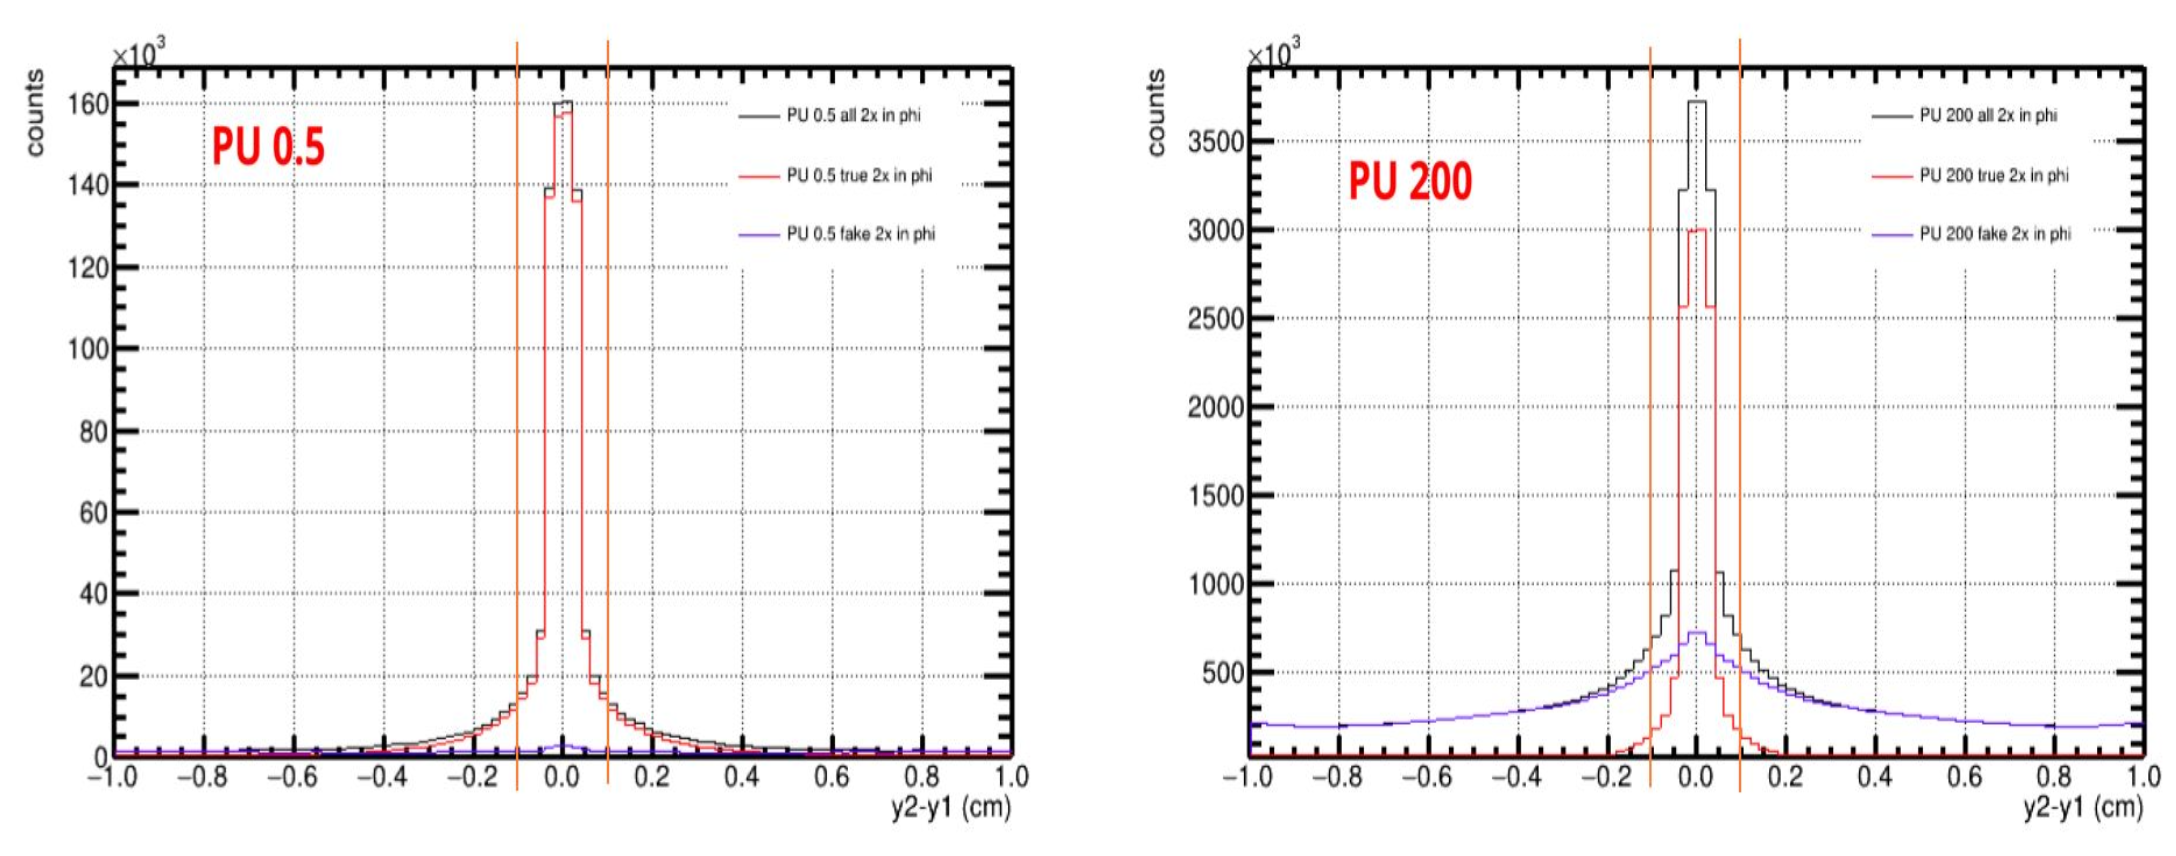
\includegraphics[width=1\textwidth]{ashish_thesis/twofoldcoin_cluster_y.png}
\caption[Total, True and Fake Two Fold Coincidences in phi (old y variables)]{%
    Separation between y coordinates of clusters in module overlap region for pileup 0.5 and 200 showing distribution total, true and fake two fold coincidences in phi.
}
\label{fig:dy_twofold}
\end{figure}

In order to reduce fake two fold coincidences for high pileup, we tried more stringent selections on separation of x, y variables for original and coincidence clusters as depicted in Fig. \ref{fig:cutopdxdy} to select dx, dy distribution (shown in Fig. \ref{fig:dx_twofold} and Fig. \ref{fig:dy_twofold}) only close to the peak cluster count but were unable to improve the residuals at high pileup to suppress physics noise. With this algorithm, we obtain residual upto 3\% even with smallest possible selection on dx and dy. Residuals obtained using different value of dx, dy selections are shown in Fig. \ref{fig:res_dxdycut}.

\begin{figure}[!htp]
\centering
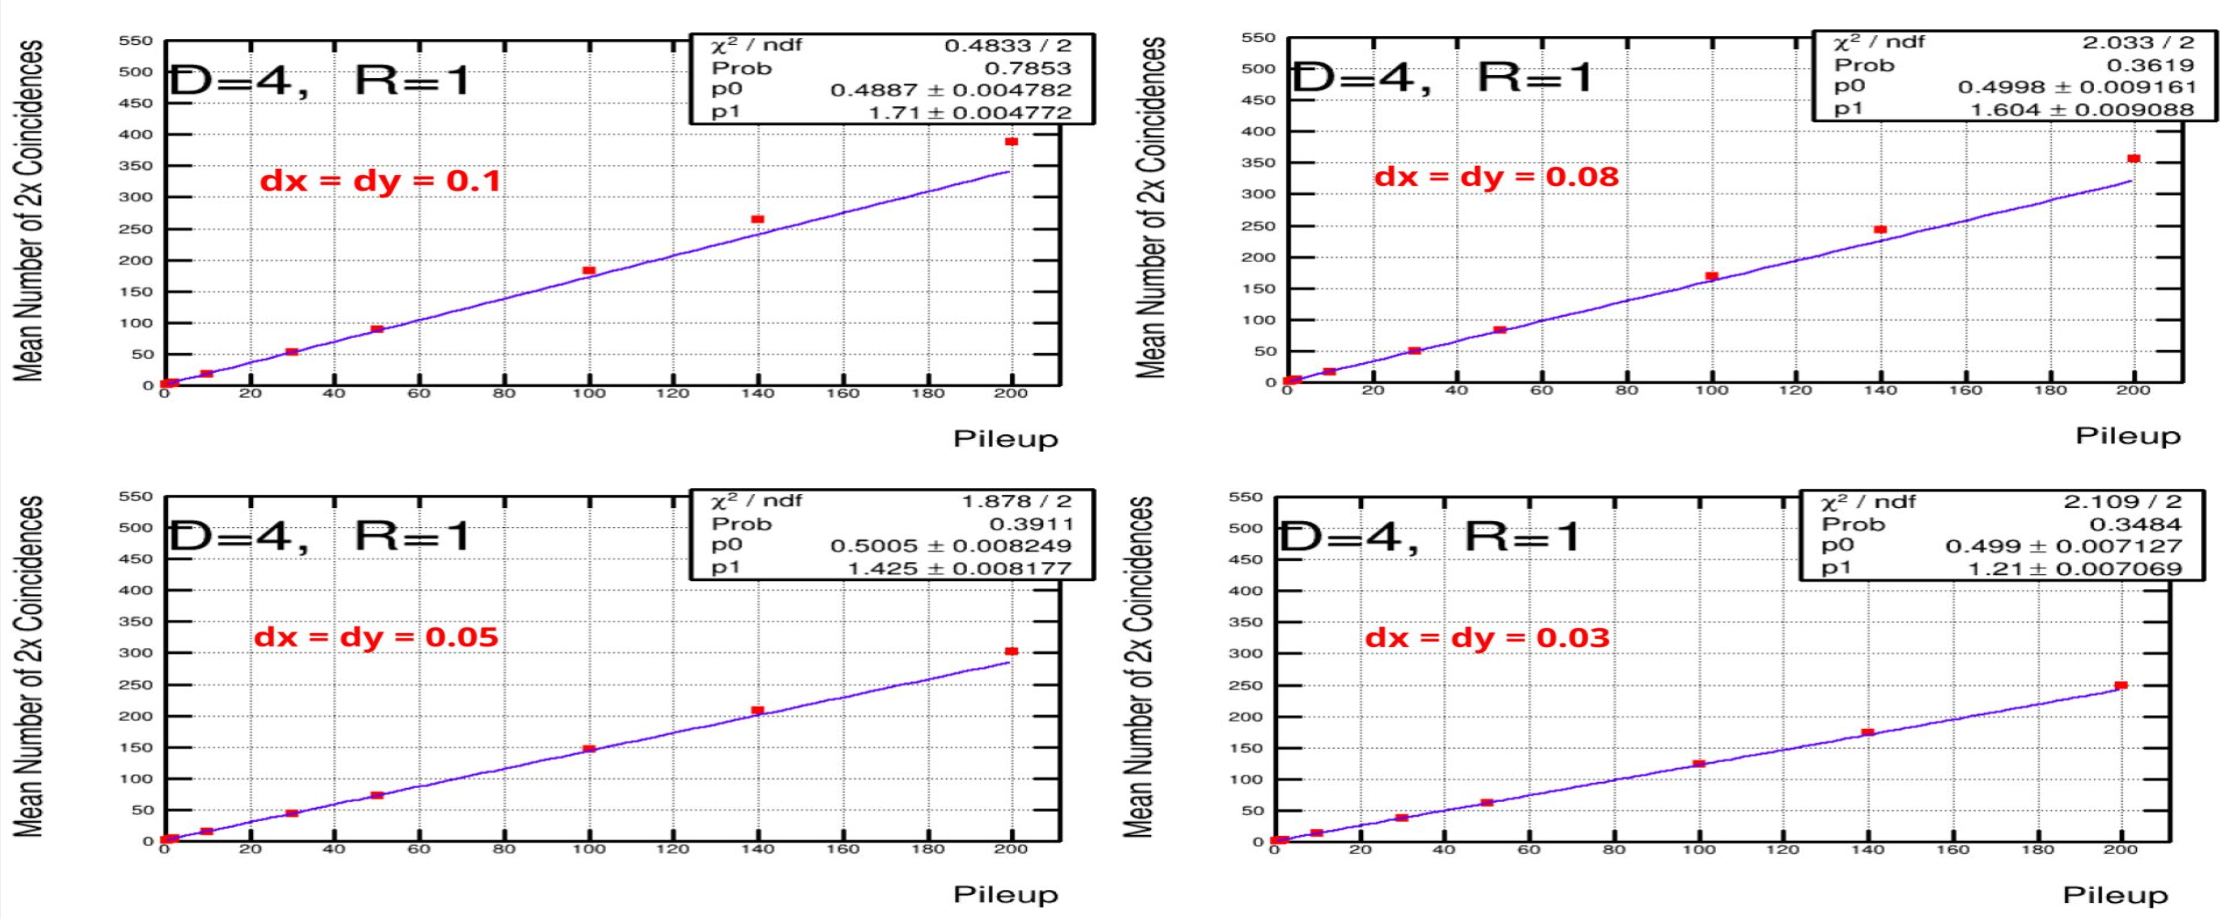
\includegraphics[width=1\textwidth]{ashish_thesis/cut_optimization_twofoldcoin.png}
\caption[Cut Optimization  Old variables]{%
 Cut optimization for two fold coincidences based on x, y variables to compute coincidence cluster separation.
}
\label{fig:cutopdxdy}
\end{figure}

\begin{figure}[!htp]
\centering
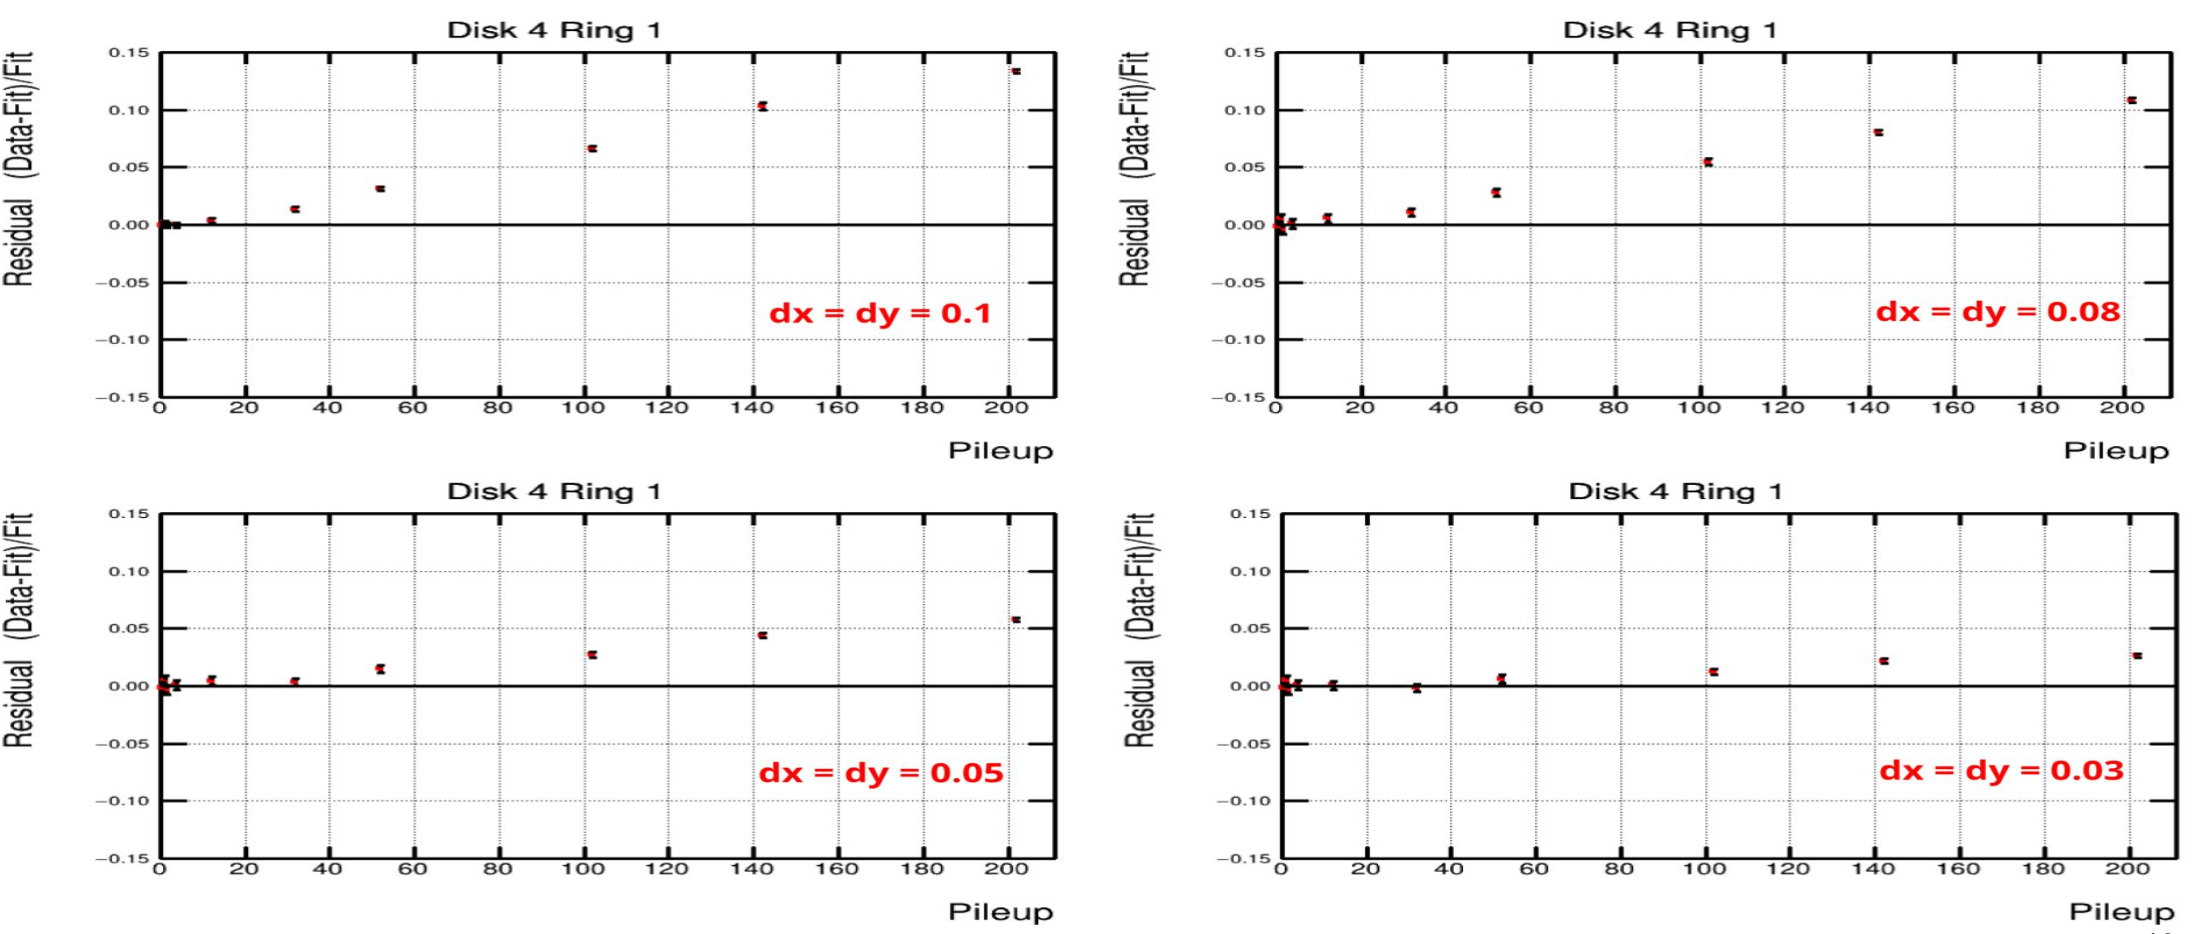
\includegraphics[width=1\textwidth]{ashish_thesis/cut_optimization_residual.png}
\caption[Residuals Different Cut Values]{%
  Residual obtained after doing linear fit for different values of dx and dy. Fake two fold coincidences does not show decrement for high pileup when more stringent selections are applied on dx, dy variables.
}
\label{fig:res_dxdycut}
\end{figure}

\end{comment}

A new algorithm for luminosity measurement based on counting two-fold coincidences is proposed that applies selections using dr and $d\phi$ variables (shown in Fig. \ref{fig:drdphi_diagram}) to minimize non-linearity for high pileup as these variables take into account track angle and its curvature \cite{sehrawat2020}.  Proper selections are applied for each TEPX disk based on these variables using low pileup simulated samples and then these selections are applied to high pileup samples for suppressing fake coincidences.


\begin{figure}[!htp]
\centering
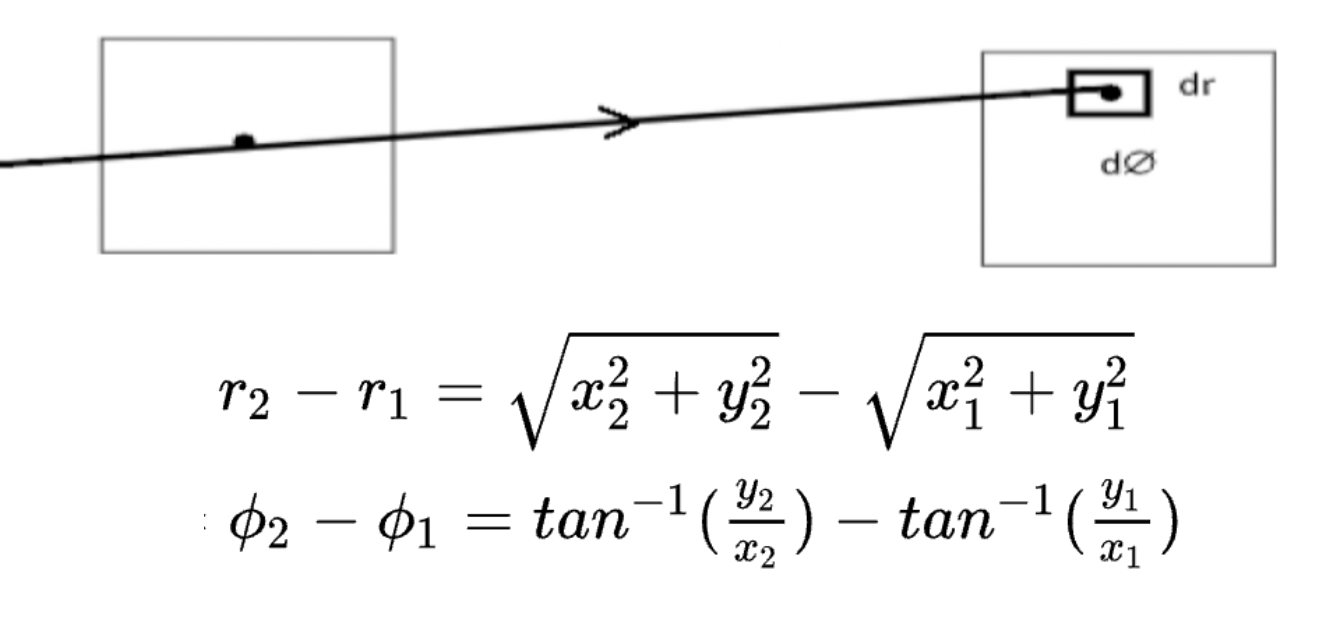
\includegraphics[width=0.7\textwidth]{ashish_thesis/dr_dphi_variables1_1.png}
\caption[New Variables For Two Fold Coincidences]{%
  r, phi variables used to define coincidence clusters. %These variables take into account track angle and curvature.
}
\label{fig:drdphi_diagram}
\end{figure}

\begin{comment}

\begin{figure}[!htp]
\centering
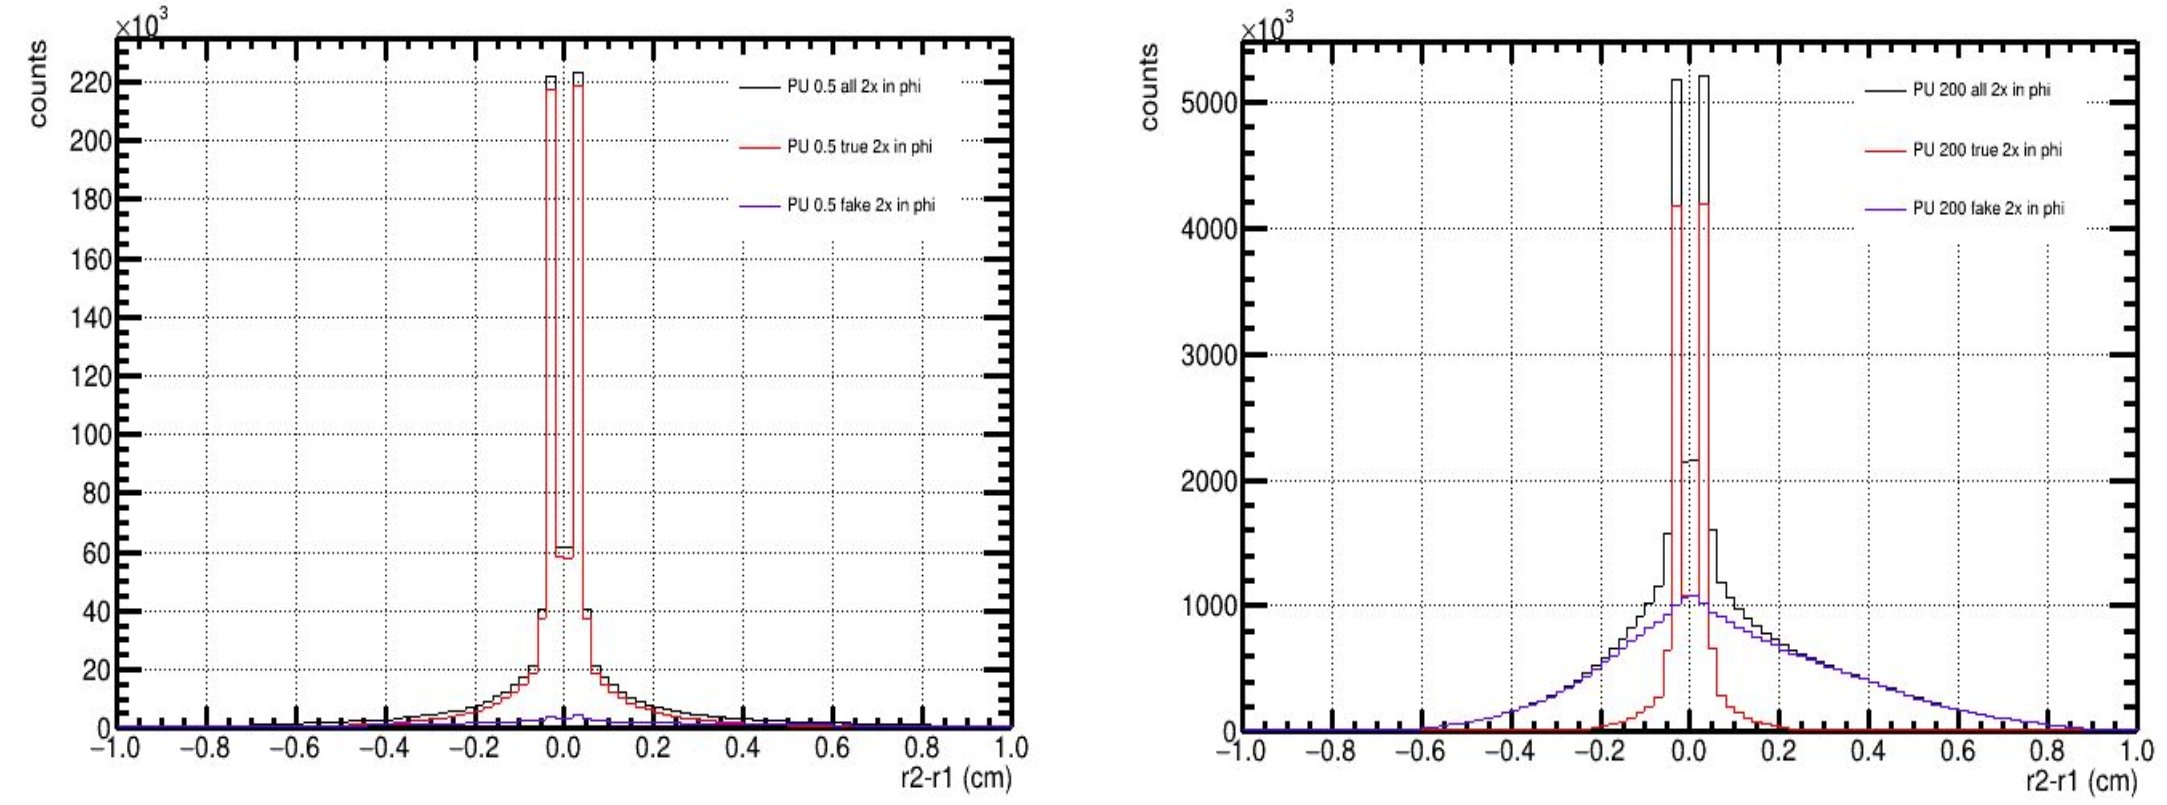
\includegraphics[width=1\textwidth]{ashish_thesis/delta_r.png}
\caption[Total, True & Fake Cluster Counts vs. dr (PU 0.5)]{%
  Distribution of total, true and fake coincidence cluster count as a function of dr variable for pileup 0.5.
}
\label{fig:dr}
\end{figure}

\begin{figure}[!htp]
\centering
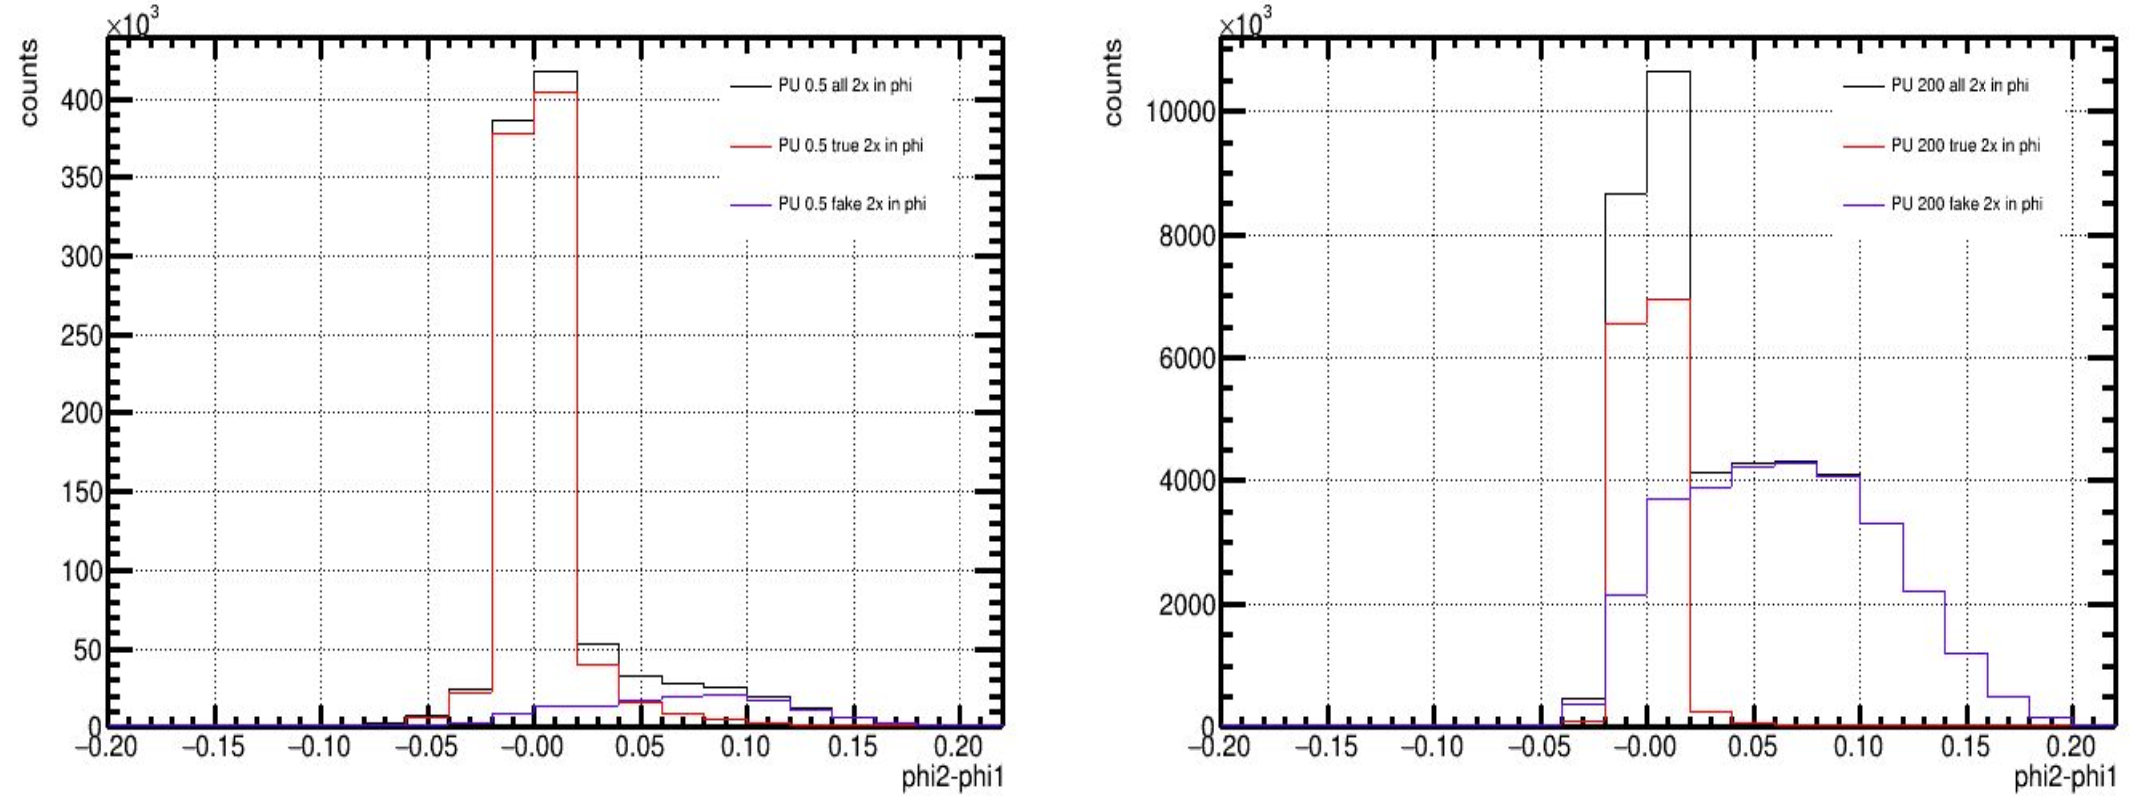
\includegraphics[width=1\textwidth]{ashish_thesis/dphi.png}
\caption[Total, True & Fake Cluster Counts vs. dphi (PU 0.5)]{%
 Distribution of total, true and fake coincidence cluster count as a function of dphi variable for pileup 0.5.
}
\label{fig:dphi}
\end{figure}

\end{comment}

We study the two-fold coincidences in $\phi$ for all TEPX Disk and rings using r, phi variable for pileup 0.5. Based on pileup 0.5 sample, a pre-selection of 0.15 mm on dr and 0.04 on dphi variable is applied in order to remove fake coincidences. 

The dr, dphi distribution showing true, fake, total two-fold coincidences for Disk 4 Ring 1 for pileup 0.5 is shown in Fig. \ref{fig:cluster_dr_dphi_dist}. After obtaining these distributions for all TEPX disks and rings, we carry out fit of the true coincidences distribution (shown in red color) to obtain mean and standard deviation of these distributions. A two-standard-deviation selection is applied on the dr value about the mean. The mean values are shown in Table \ref{tab:mdr_cuts_offset_values}. The  standard deviation values of the fit to true coincidences for all disks and rings are shown in Table \ref{tab:disk_values}. %Example fits are shown in Fig. \ref{fig:cluster_ring_1003}, \ref{fig:cluster_ring_70}, \ref{fig:cluster_ring_71}. 
Similarly, two-sigma cut is applied on the dphi variable as well. The standard deviation values for dphi variable are shown in Table \ref{tab:mdphi_cuts_values}. While doing the fit, mean value for dphi variable is set to zero. %The mean is taken as the offset value and standard deviation is used as the selection on dr, dphi variables as shown in Table \ref{tab:disk_values}, \ref{tab:mdphi_cuts_values} and \ref{tab:mdr_cuts_offset_values}. 
%The mean of the fit is taken as the offset value and standard deviation is used as the cut on dr, dphi variables.
A plot of two-fold coincidences in phi after applying all selection based on standard deviation values of all TEPX disks and rings is shown in Fig. \ref{fig:cluster_ring_720}.

\begin{figure}[H]
\centering
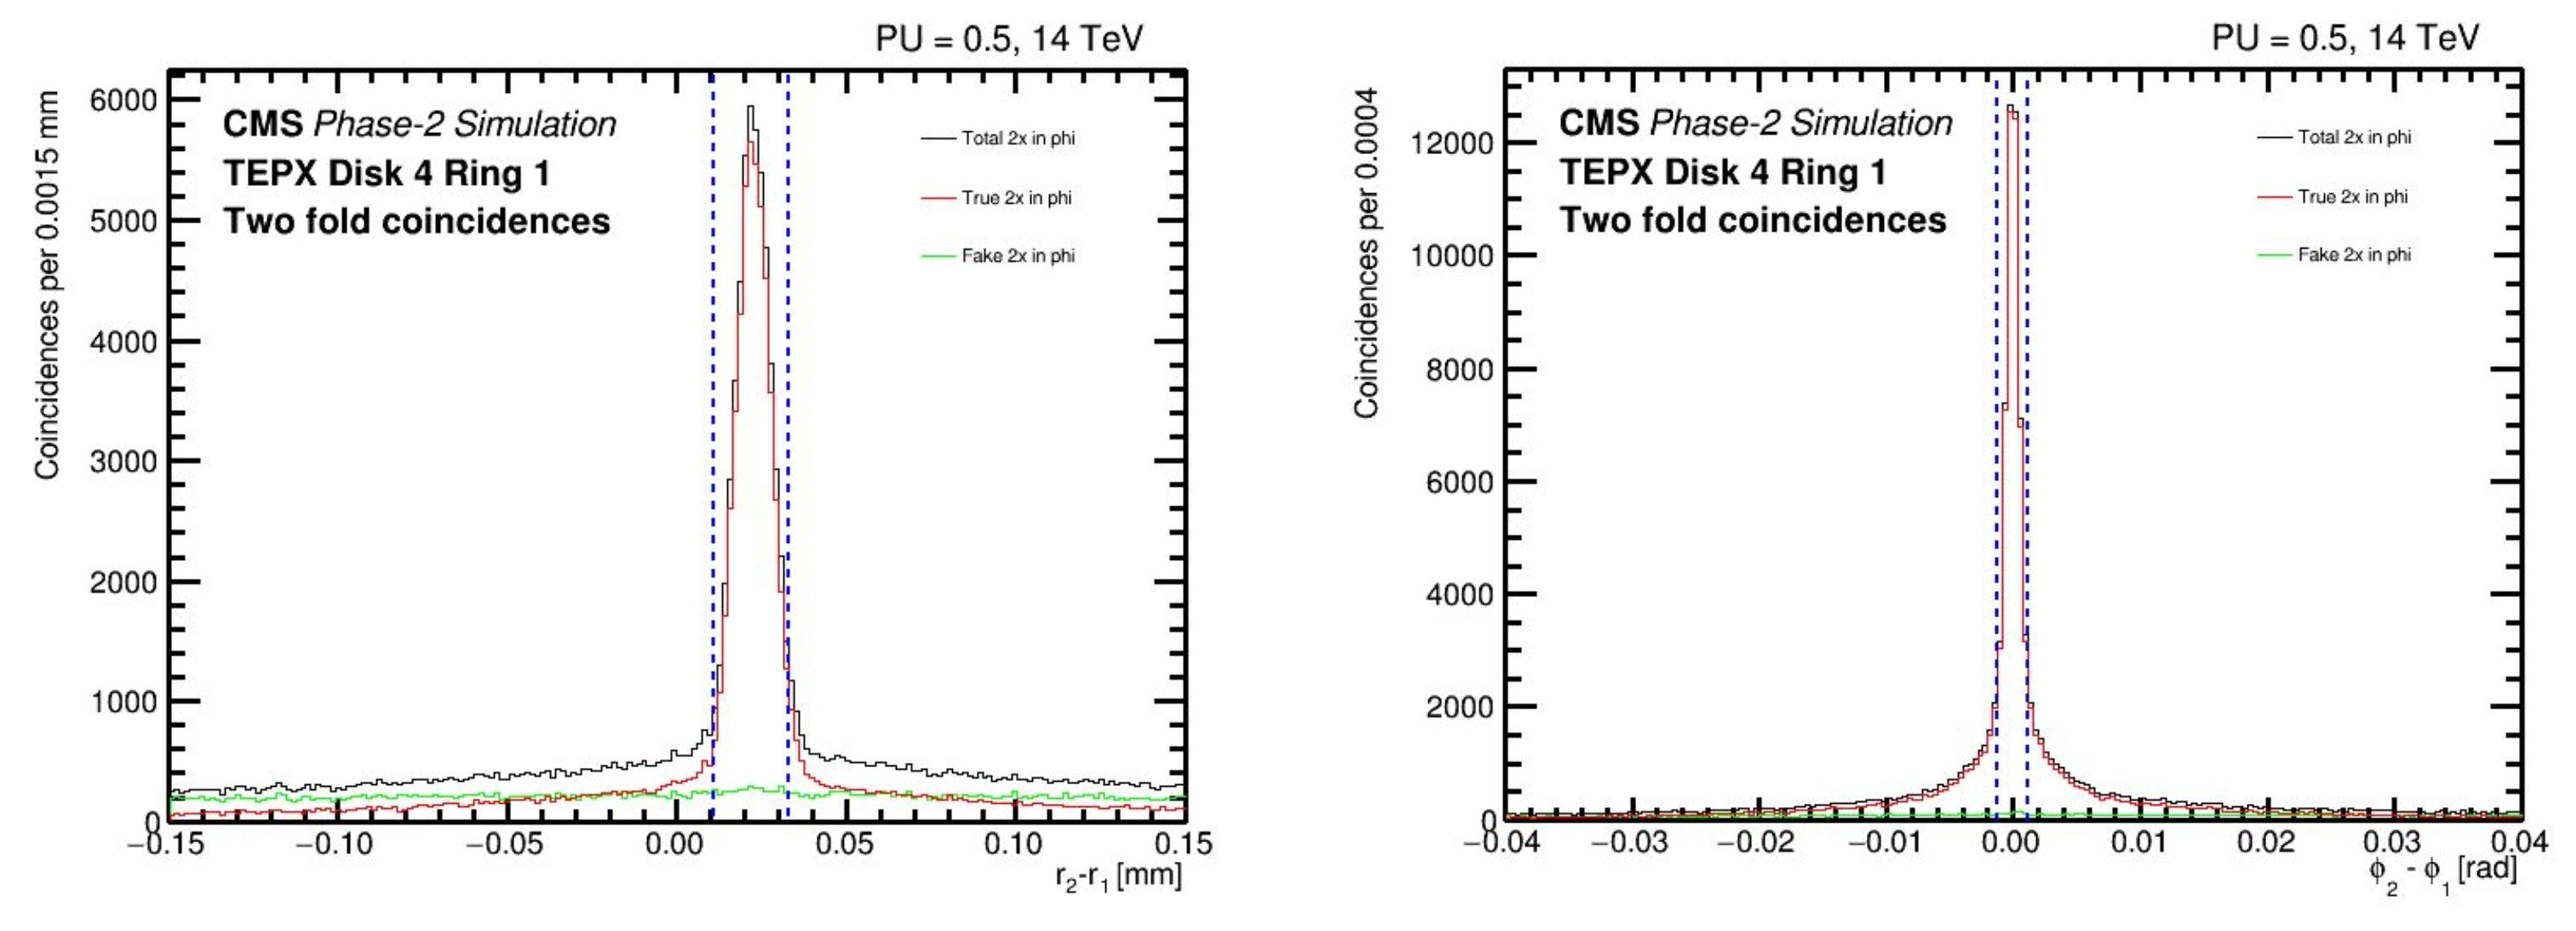
\includegraphics[width=1\textwidth]{ashish_thesis/D4R1_S2_drdphi_cut_2.png}
\caption[Pileup 0.5 Cluster Count in D4R1 vs. dr & dphi]{%
  Distribution of cluster count as a function of dr and dphi variables for pileup 0.5 for Disk 4 Ring 1. The black curve represents the total two-fold coincidence counts, the red curve depicts the true two-fold coincidence counts, and the green curve indicates the fake two-fold coincidence counts.
}
\label{fig:cluster_dr_dphi_dist}
\end{figure}


\begin{comment}

\begin{figure}[!htp]
\centering
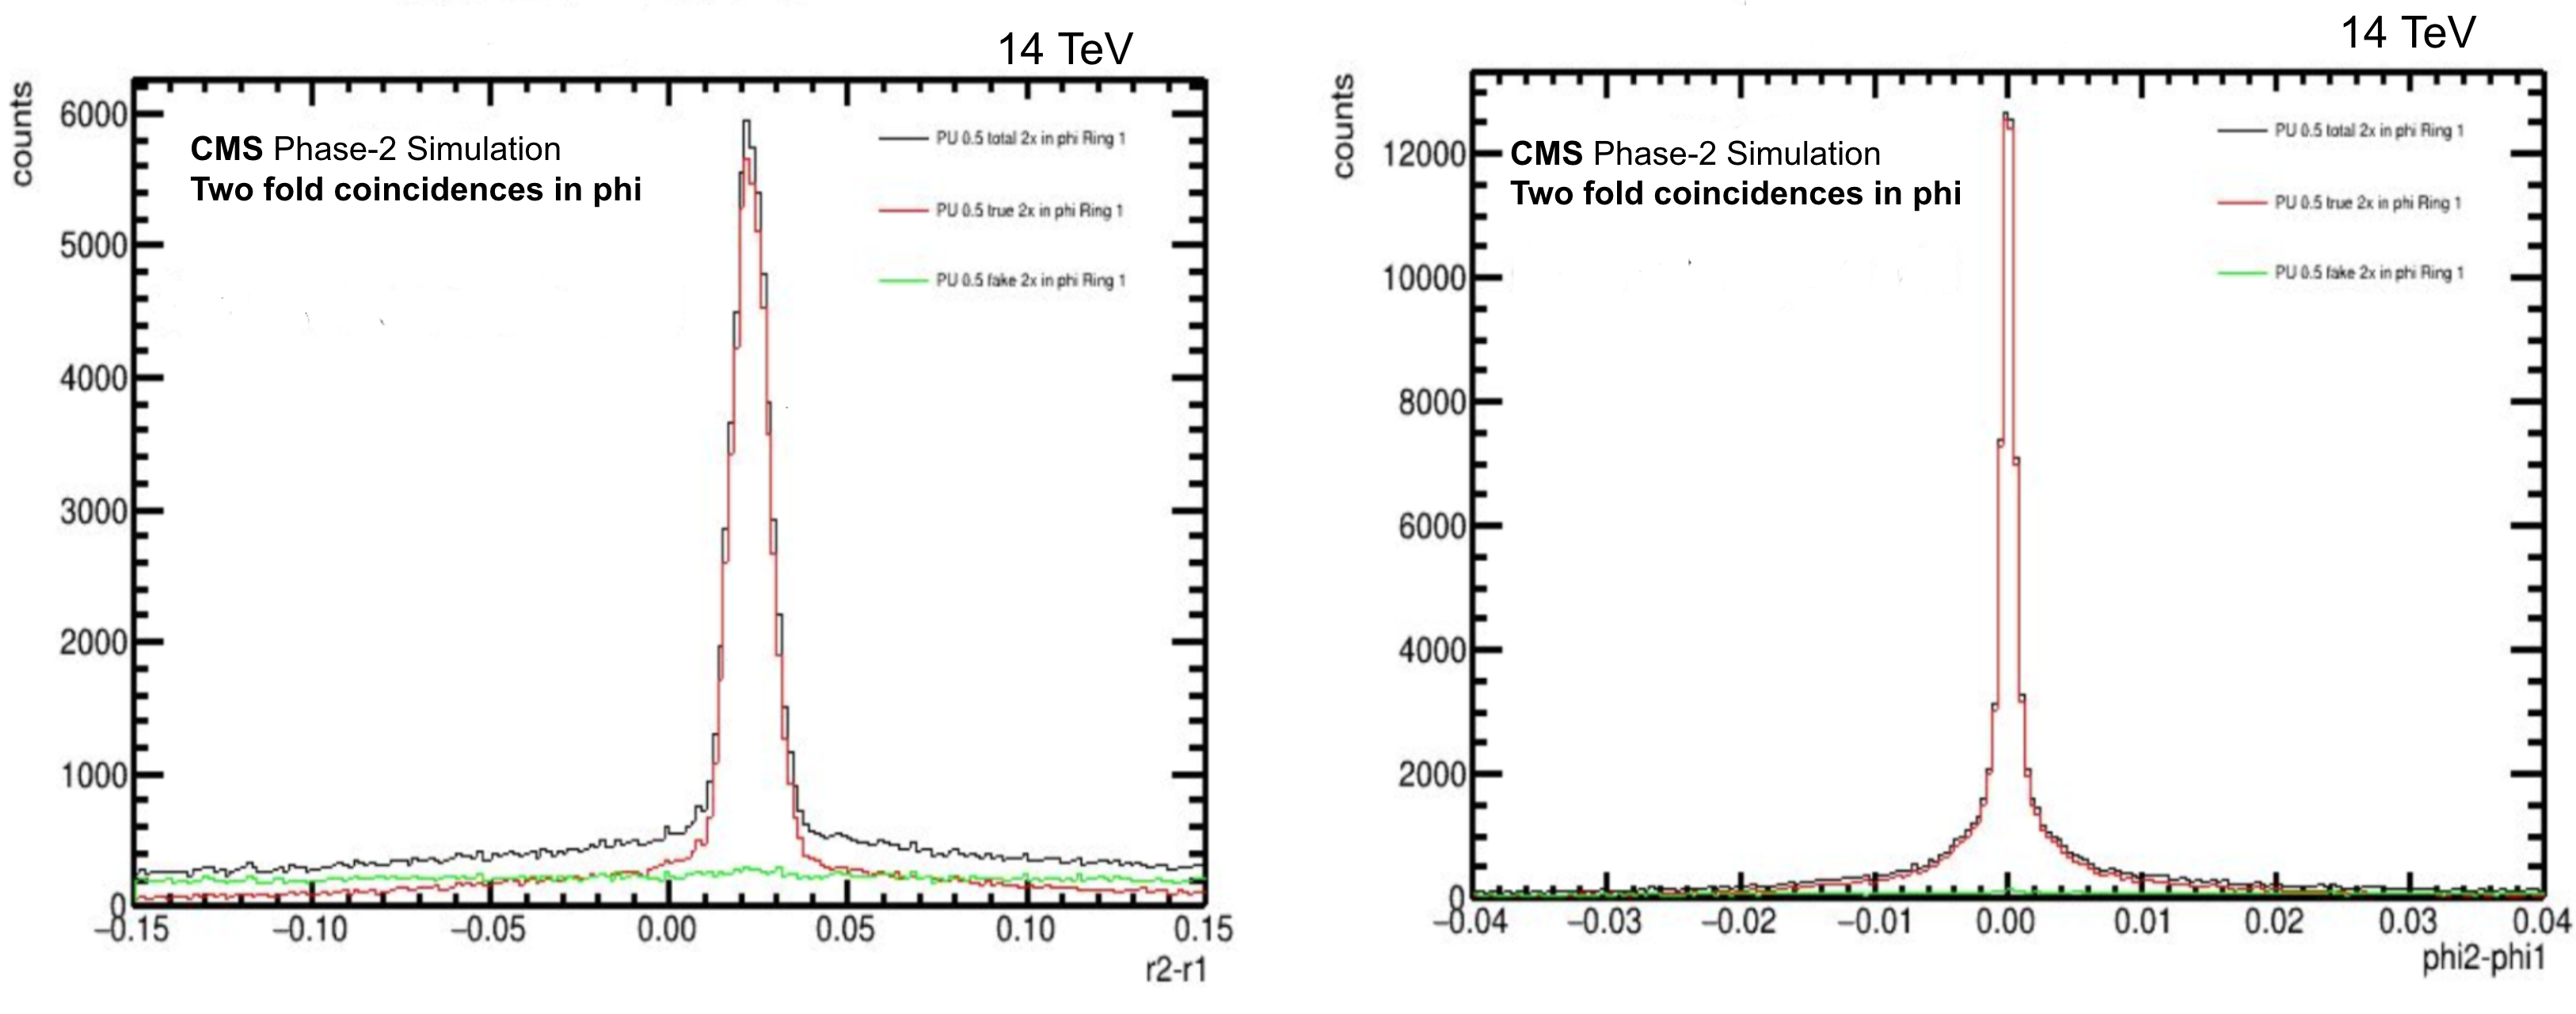
\includegraphics[width=1\textwidth]{ashish_thesis/D4R1_S2_drdphi_cut.png}
\caption[Pileup 0.5 Cluster Count in D4R1 (+Z) vs. dr & dphi]{%
  Distribution of cluster count as a function of dr and dphi variables for pileup 0.5 for disk 4 Ring 1 (+Z). Appropriate selection on dr, dphi are used to minimize fake two fold coincidences.
}
\label{fig:cluster_dr_dphi_dist}
\end{figure}


\begin{figure}[!htp]
\centering
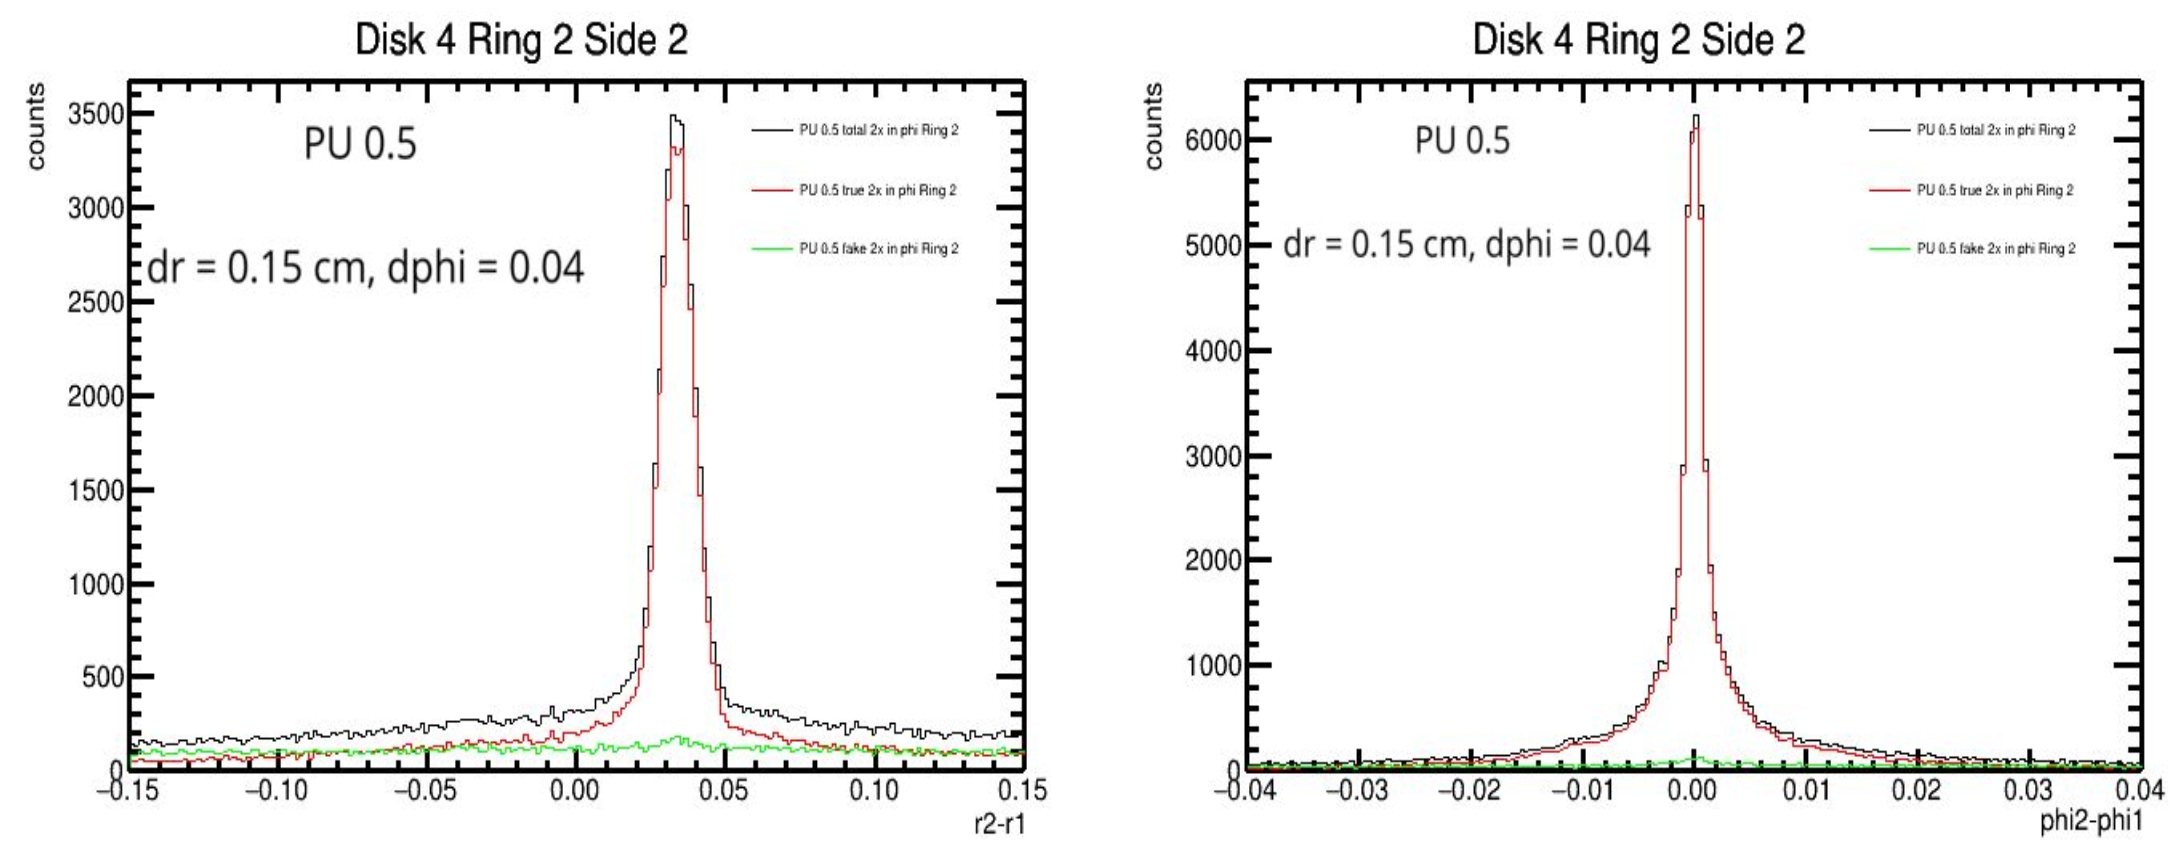
\includegraphics[width=1\textwidth]{ashish_thesis/D4R2_S2_drdphicut.png}
\caption[Pileup 0.5 Cluster Count in D4R2 (+Z) vs. dr & dphi]{%
   Distribution of cluster count as a function of dr and dphi variables for pileup 0.5 for disk 4 Ring 2 (+Z). Appropriate selection on dr, dphi are used to minimize fake two fold coincidences.
}
\label{fig:cluster_ring_1000}
\end{figure}


\begin{figure}[!htp]
\centering
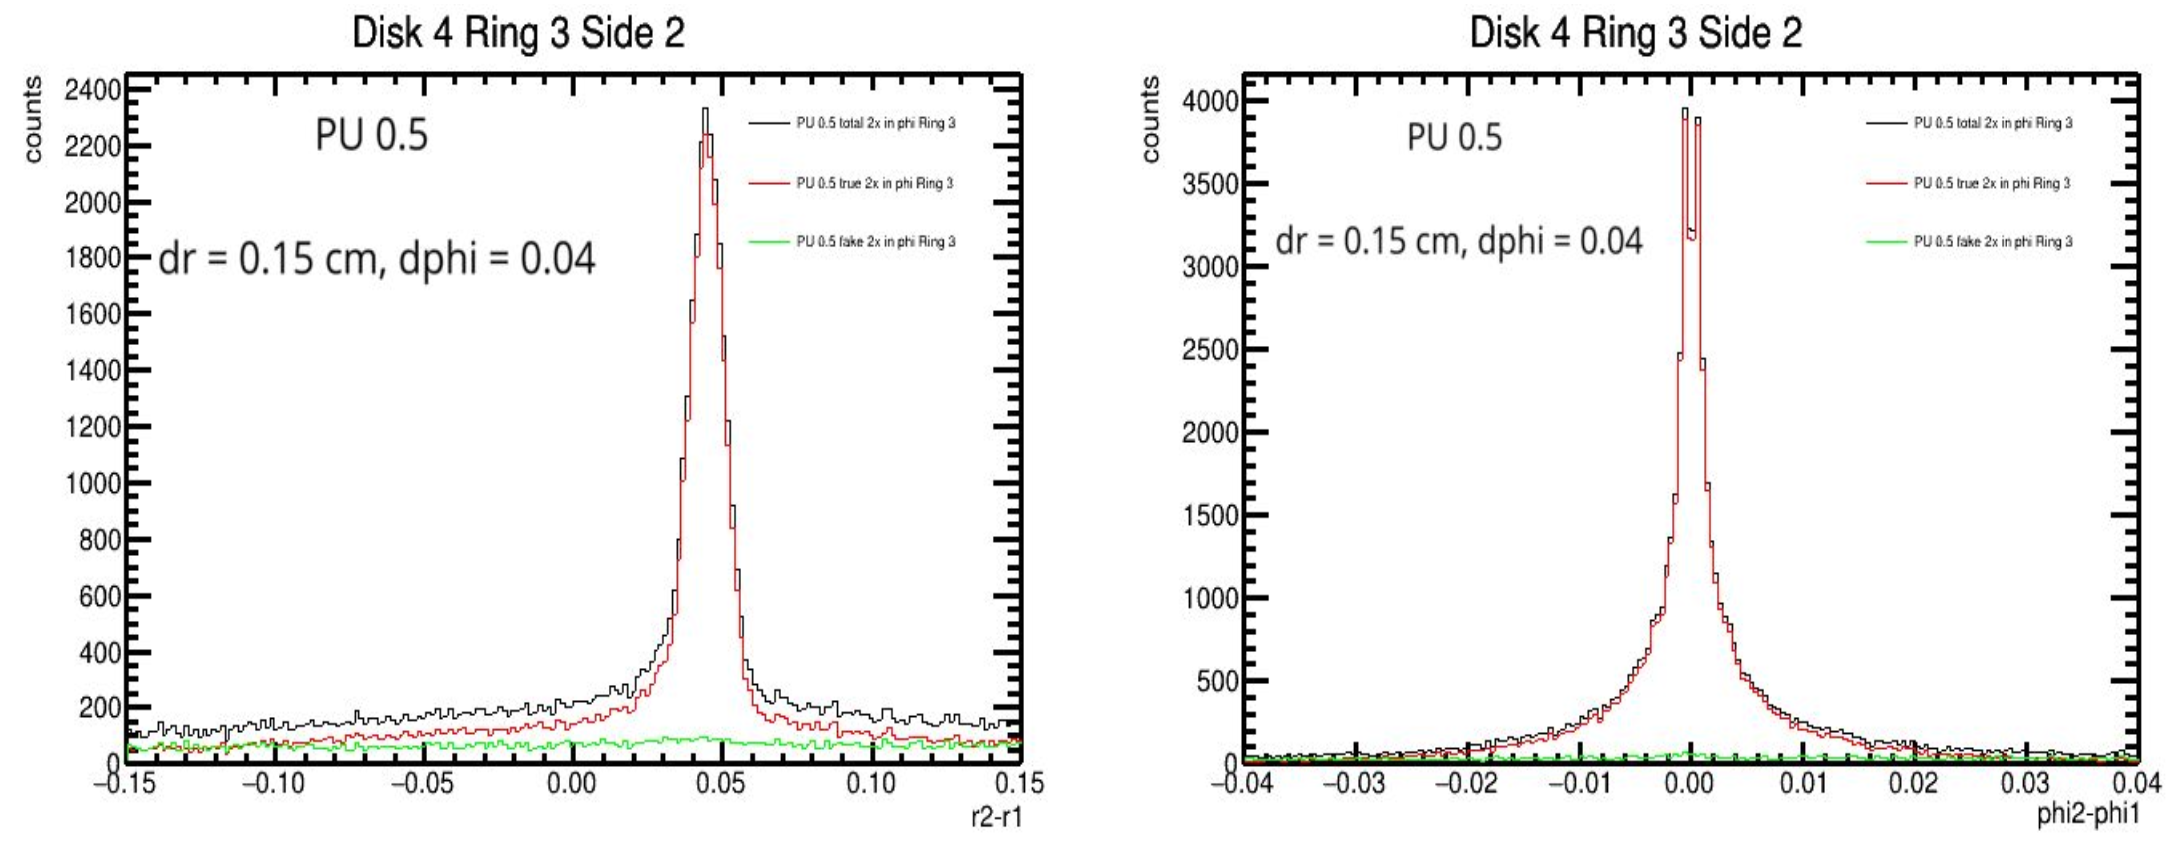
\includegraphics[width=1\textwidth]{ashish_thesis/D4R3_S2_drdphi_cut.png}
\caption[Pileup 0.5 Cluster Count in D4R3 (+Z) vs. dr & dphi]{%
  Distribution of cluster count as a function of dr and dphi variables for pileup 0.5 for disk 4 Ring 3 (+Z). Appropriate selection on dr, dphi are used to minimize fake two fold coincidences.
}
\label{fig:cluster_ring_10001}
\end{figure}


\begin{figure}[!htp]
\centering
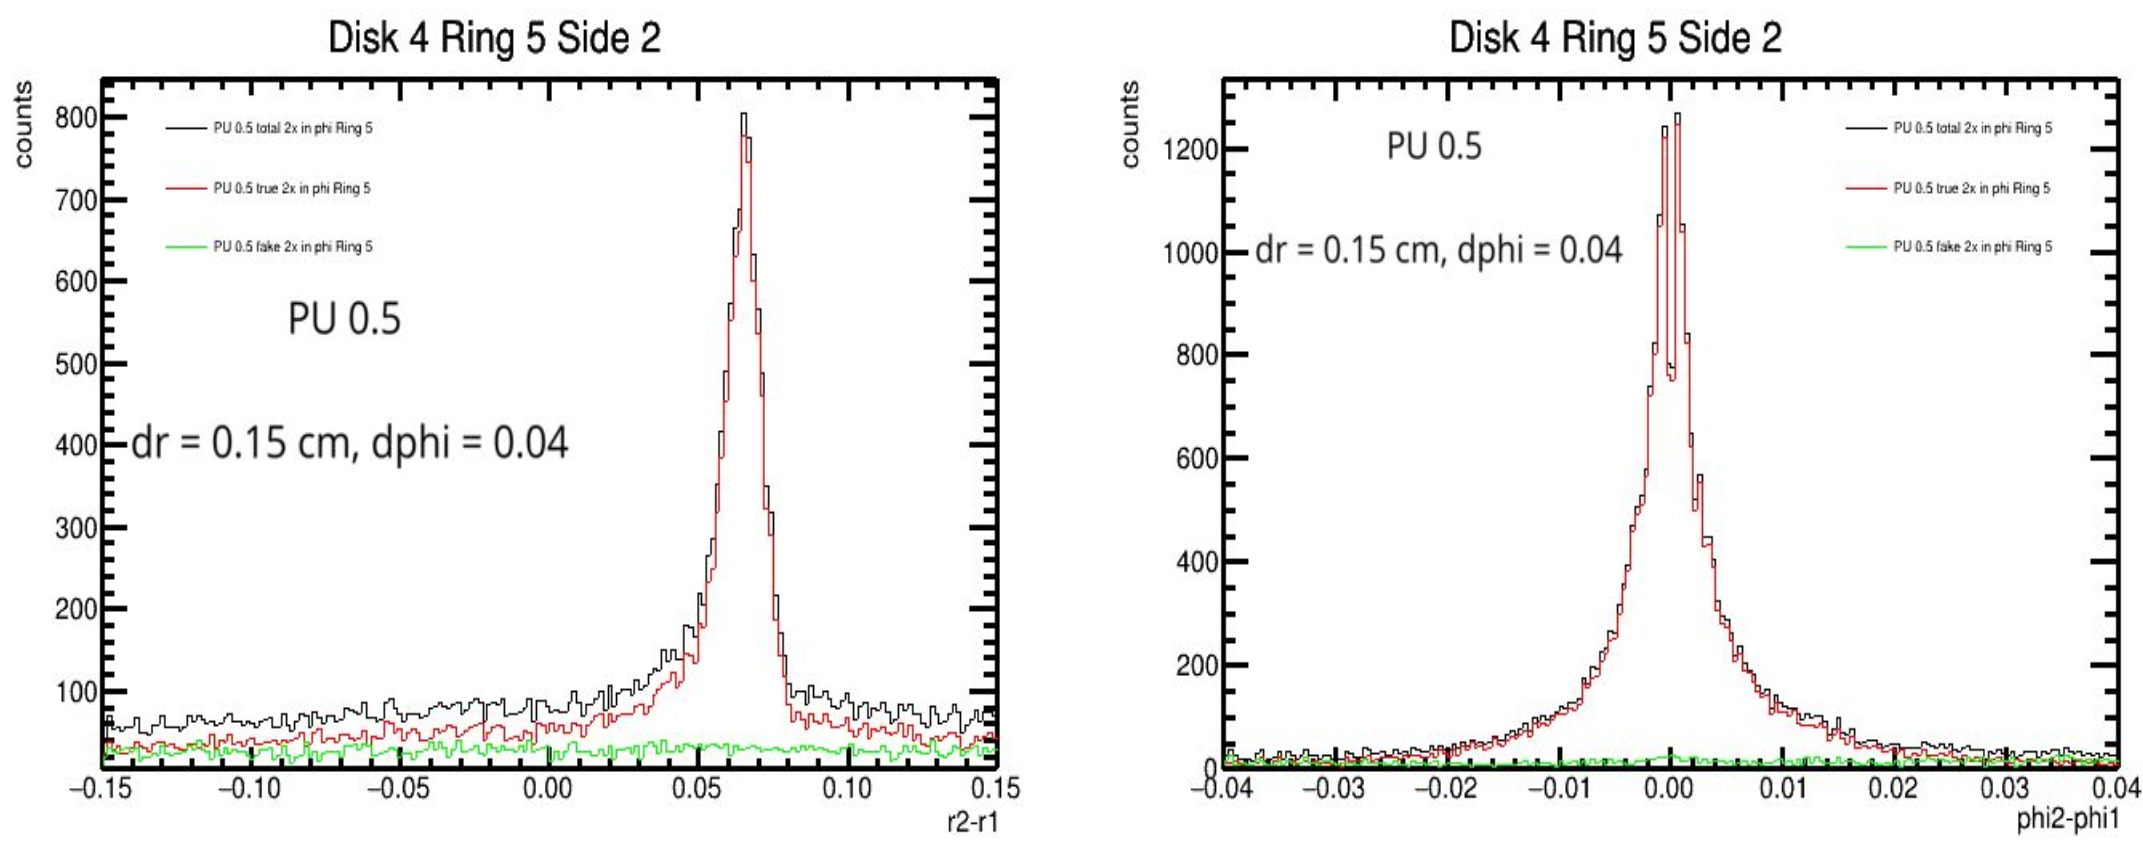
\includegraphics[width=1\textwidth]{ashish_thesis/D4R5_drdphicut.png}
\caption[Pileup 0.5 Cluster Count in D4R5 (+Z) vs. dr & dphi]{%
  Distribution of cluster count as a function of dr and dphi variables for pileup 0.5 for disk 4 Ring 5 (+Z). Appropriate selection on dr, dphi are used to minimize fake two fold coincidences.
}
\label{fig:cluster_ring_1002}
\end{figure}


\begin{figure}[!htp]
\centering
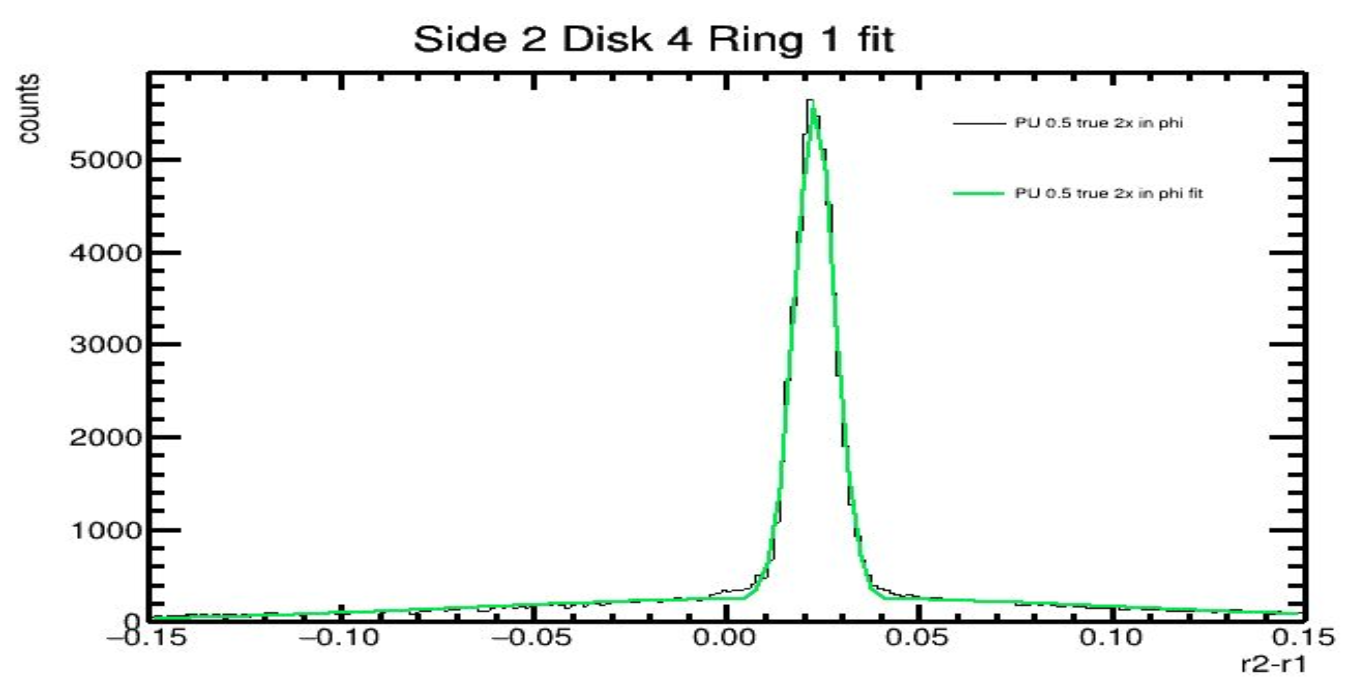
\includegraphics[width=1\textwidth]{ashish_thesis/D4R1S2_fit.png}
\caption[Disk 4 Ring 1 Clusters Fit]{%
   Example fit using single gaussian function of cluster count as a function of dr variable for Disk 4 Ring 1 (+Z).
}
\label{fig:cluster_ring_1003}
\end{figure}

\begin{comment}
  
\begin{figure}[!htp]
\centering
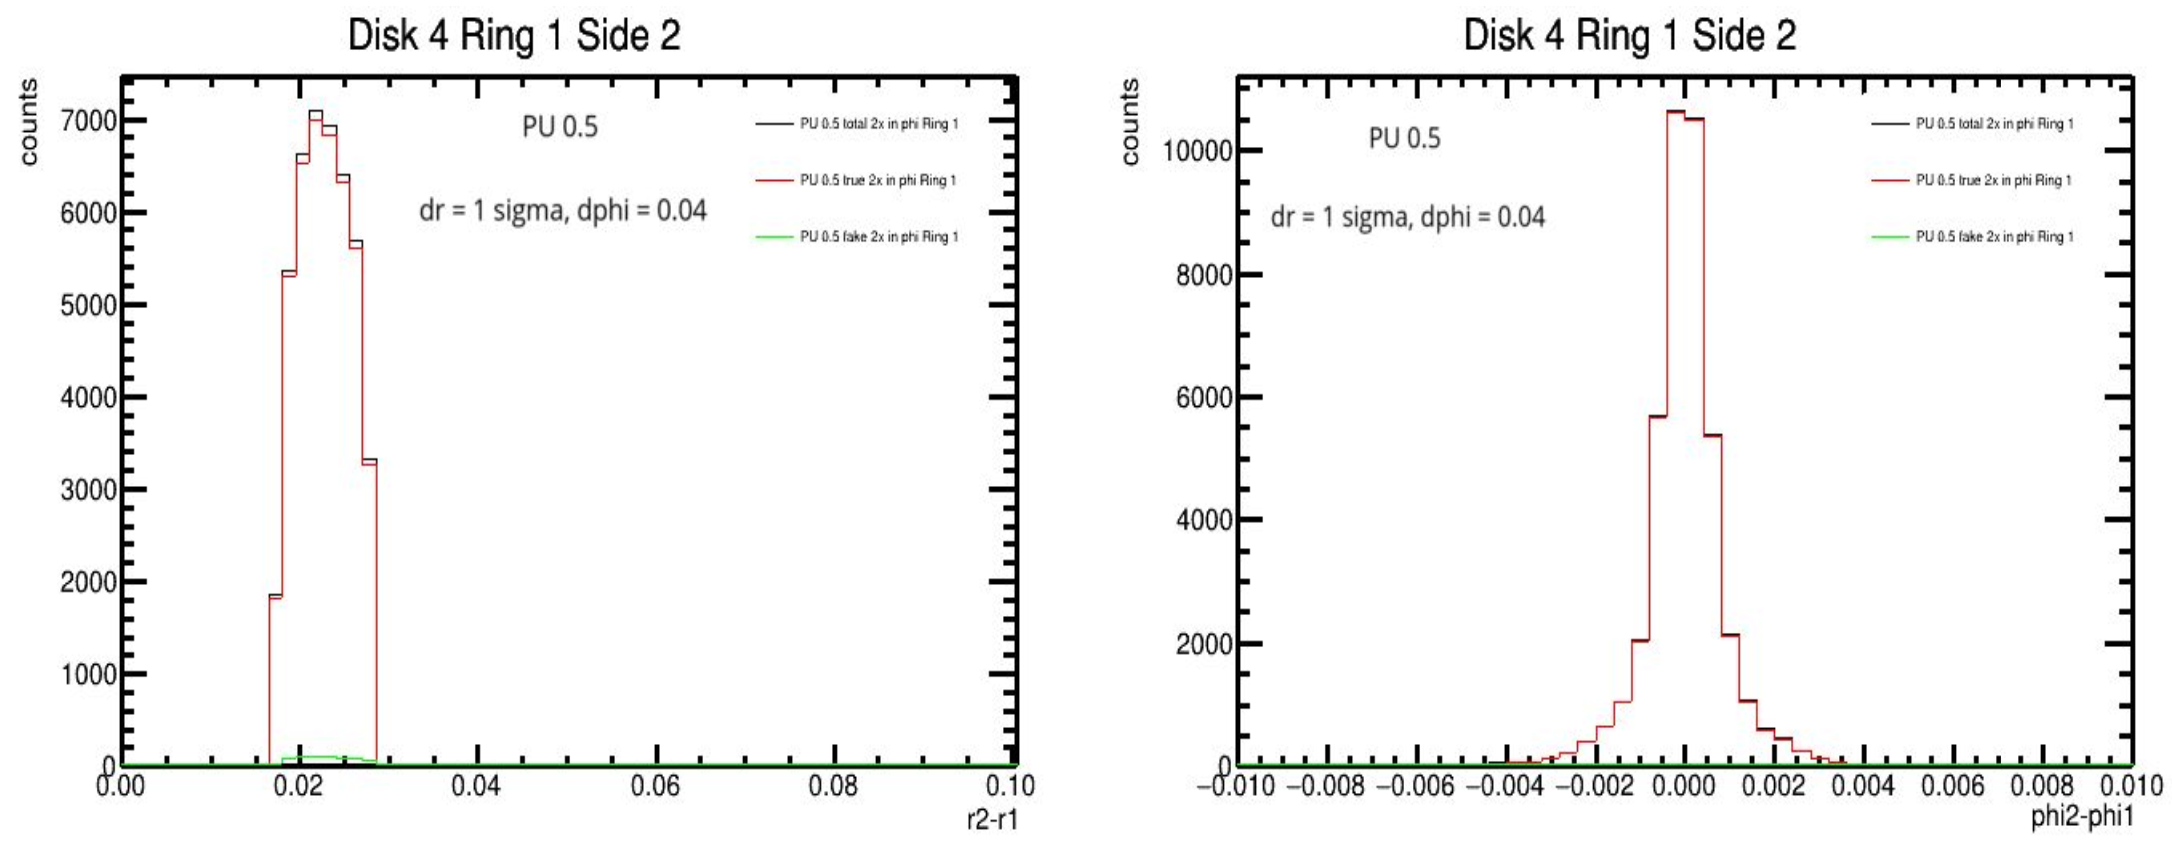
\includegraphics[width=1\textwidth]{ashish_thesis/D4R1S2_dr_dphi_cut.png}
\caption[New dr selection value]{%
 Distribution of cluster count as a function of dr and dphi variables for pileup 0.5 for disk 4 Ring 1 (+Z). 1 sigma selection on dr and dphi equal to 0.04 are used to minimize fake two fold coincidence.
}
\label{fig:cluster_ring_1004}
\end{figure}

\begin{figure}[!htp]
\centering
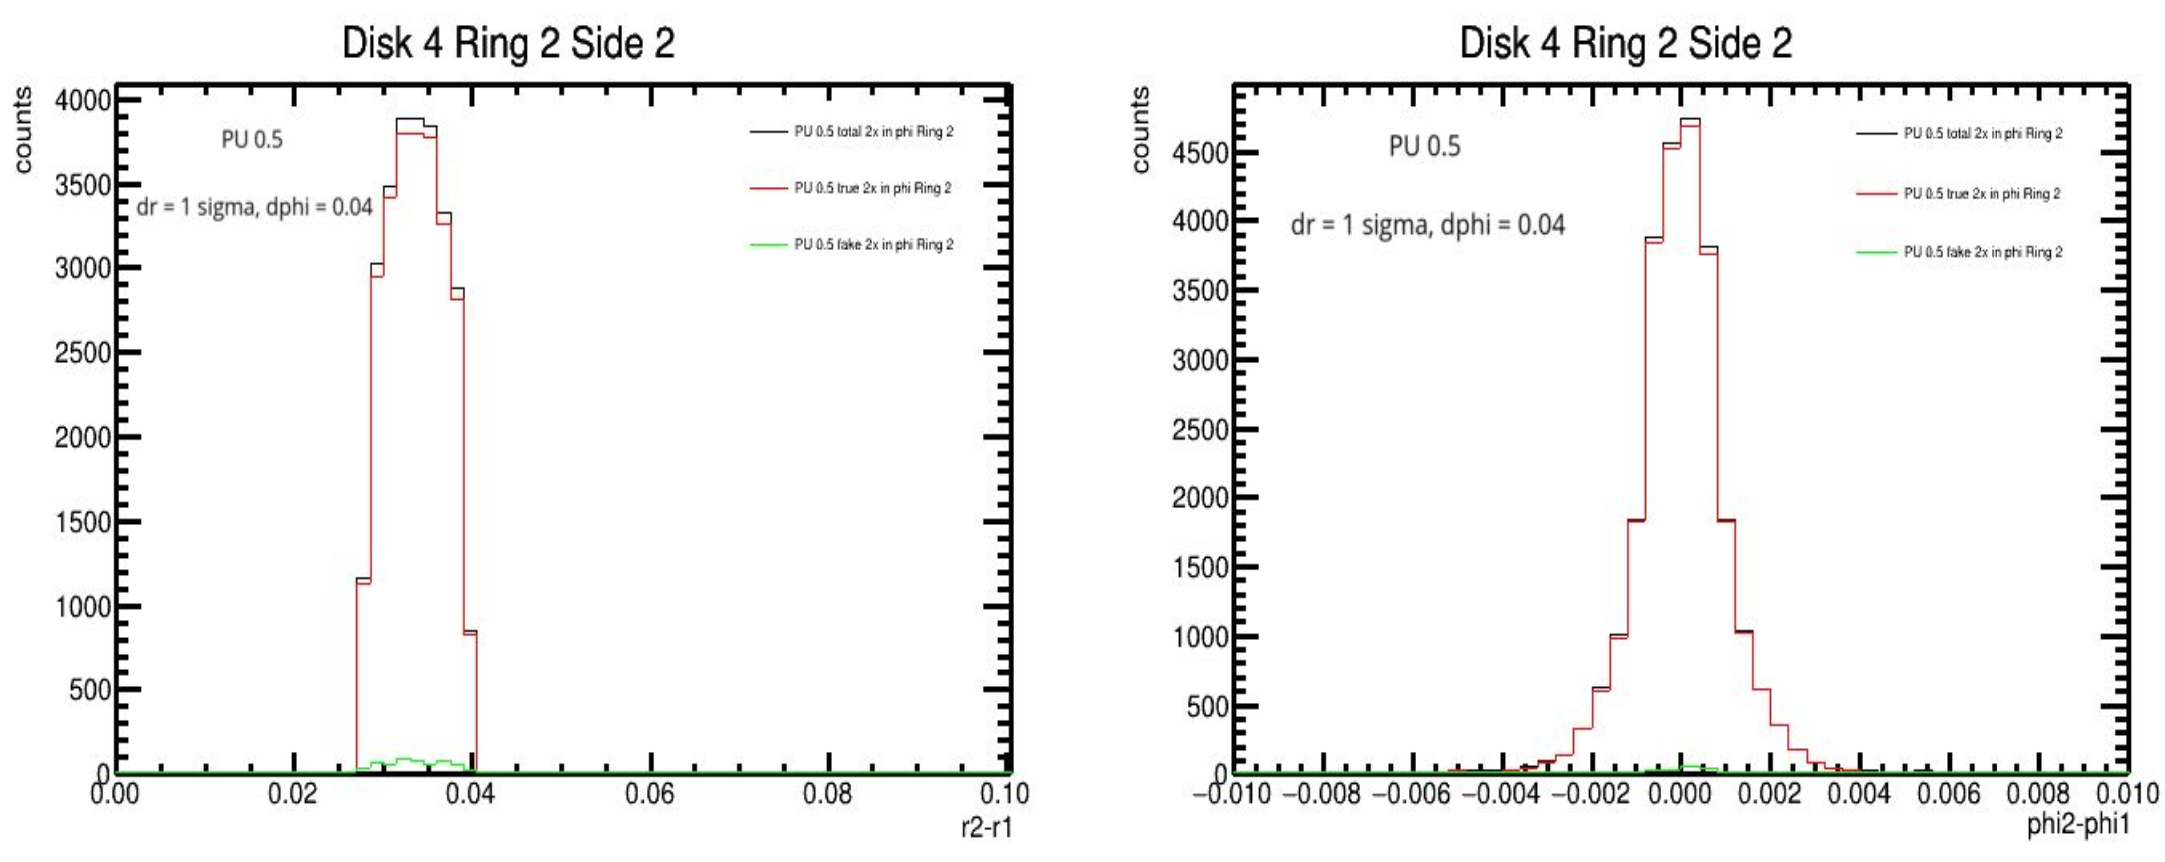
\includegraphics[width=1\textwidth]{ashish_thesis/D4R2S2_dr_dphi_cut.png}
\caption[New dphi selection value]{%
   Distribution of cluster count as a function of dr and dphi variables for pileup 0.5 for disk 4 Ring 2 (+Z). 1 sigma selection on dr and dphi equal to 0.04 are used to minimize fake two fold coincidences.
}
\label{fig:cluster_ring_1005}
\end{figure}


\begin{figure}[!htp]
\centering
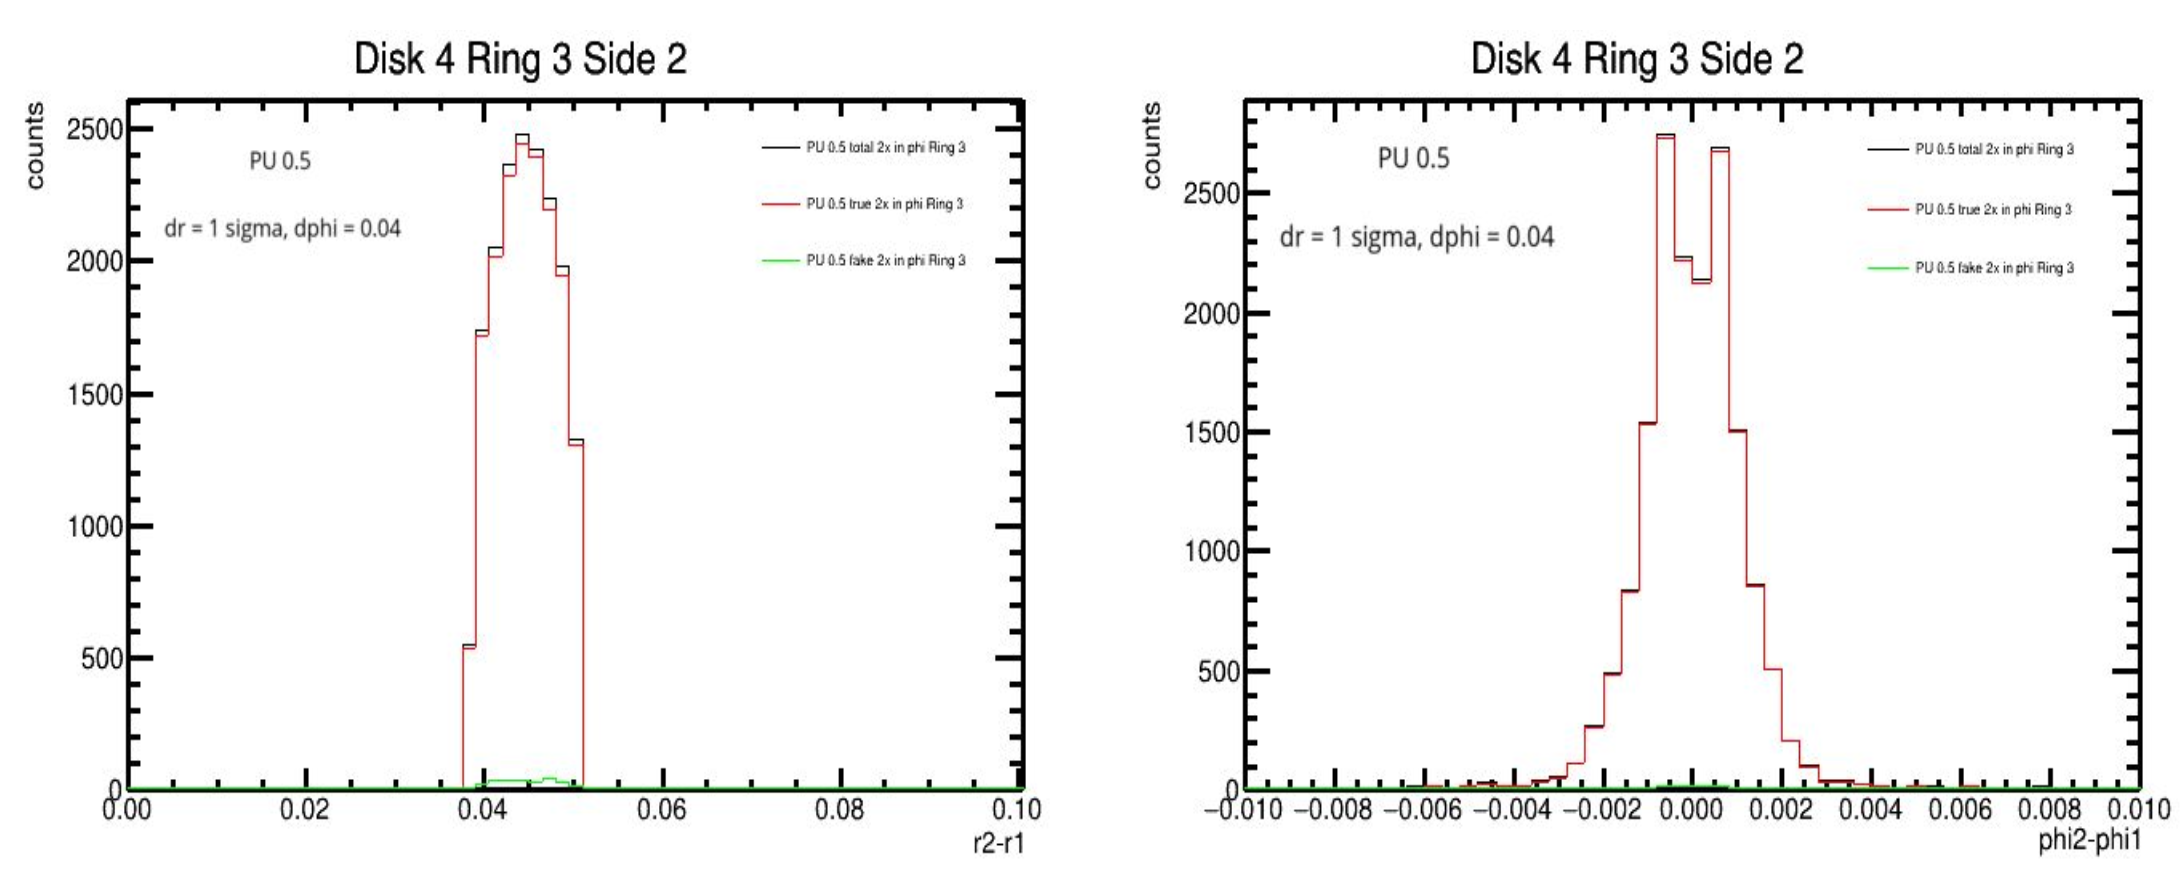
\includegraphics[width=1\textwidth]{ashish_thesis/D4R3S2_dr_dphi_cut.png}
\caption[Cluster count as function of new variables with selection for PU 0.5 D4R3S2]{%
    Distribution of cluster count as a function of dr and dphi variables for pileup 0.5 for disk 4 Ring 3 (+Z). 1 sigma selection on dr and dphi equal to 0.04 are used to minimize fake two fold coincidences.
}
\label{fig:cluster_ring_1006}
\end{figure}


\begin{figure}[!htp]
\centering
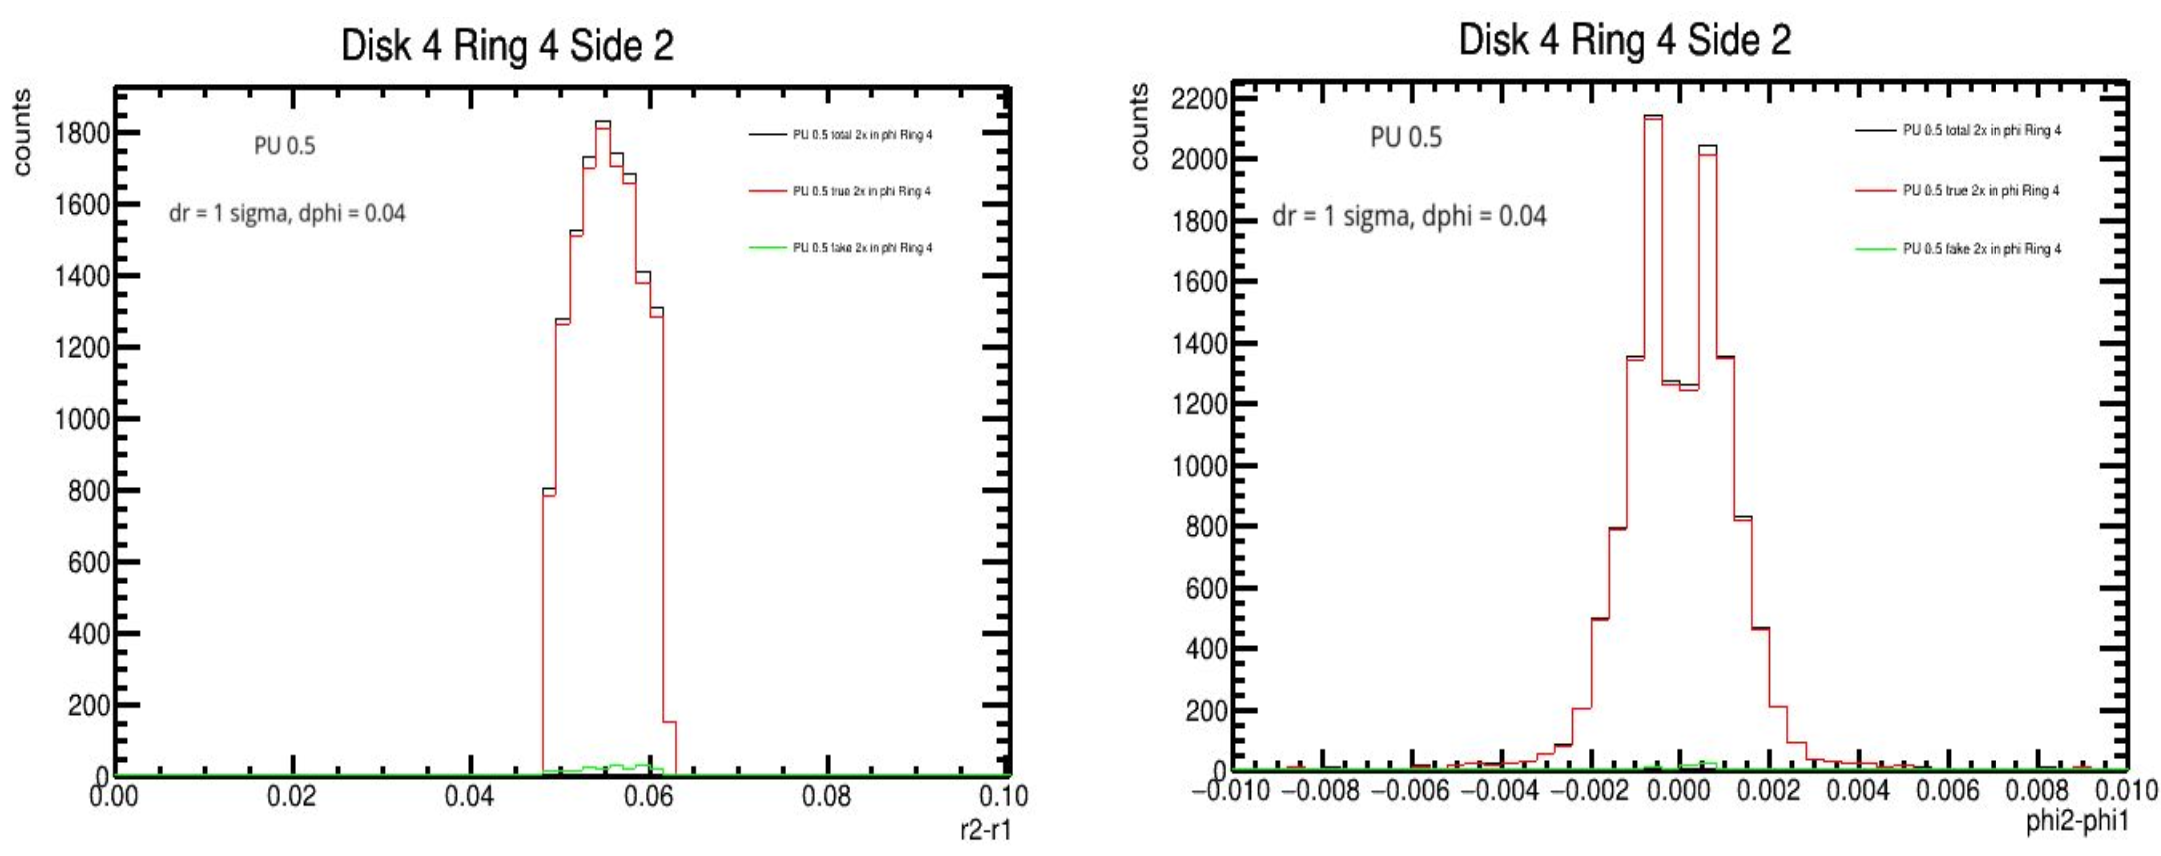
\includegraphics[width=1\textwidth]{ashish_thesis/D4R4S2_dr_dphi_cut.png}
\caption[Cluster count as function of new variables with selection for PU 0.5 D4R4S2]{%
  Distribution of cluster count as a function of dr and dphi variables for pileup 0.5 for disk 4 Ring 4 (+Z). 1 sigma selection on dr and dphi equal to 0.04 are used to minimize fake two fold coincidences.  
}
\label{fig:cluster_ring_68}
\end{figure}


\begin{figure}[!htp]
\centering
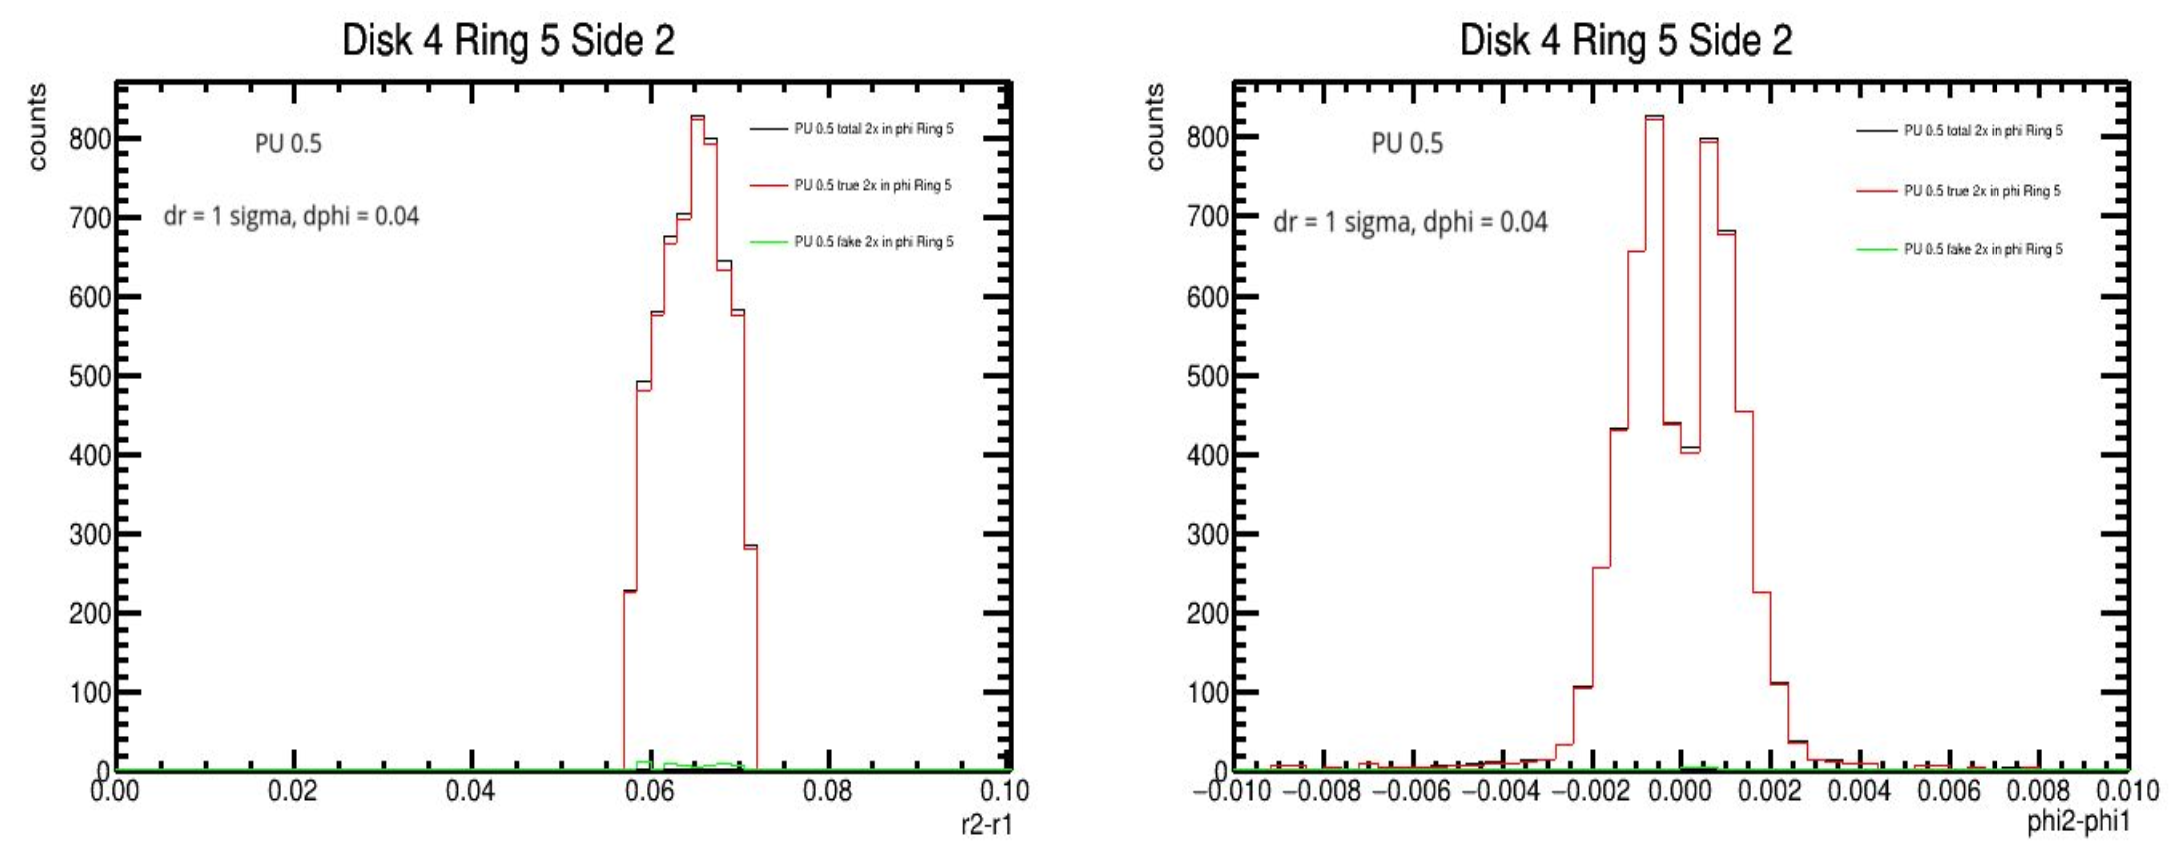
\includegraphics[width=1\textwidth]{ashish_thesis/D4R5S2_dr_dphi_cut.png}
\caption[Cluster count as function of new variables with selection for PU 0.5 D4R5S2]{%
  Distribution of cluster count as a function of dr and dphi variables for pileup 0.5 for disk 4 Ring 5 (+Z). 1 sigma selection on dr and dphi equal to 0.04 are used to minimize fake two fold coincidence clusters.  
}
\label{fig:cluster_ring_69}
\end{figure}

%\end{comment}


\begin{figure}[!htp]
\centering
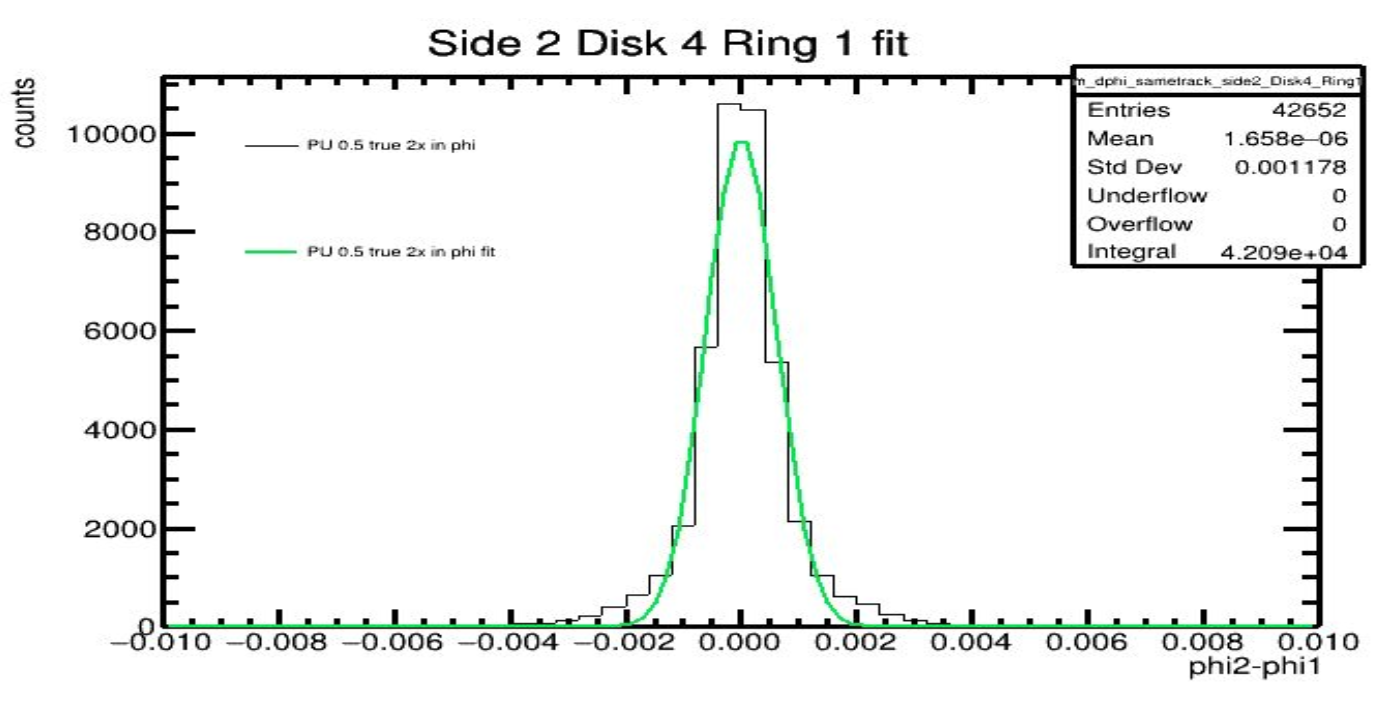
\includegraphics[width=1\textwidth]{ashish_thesis/D4R1S2_fit_PU0p5.png}
\caption[Fit Disk 4 Ring 1 (+Z) Cluster Distribution]{%
  Example fit using single Gaussian function of cluster count as a function of dphi variable for pileup 0.5 Disk 4 Ring 1 (+Z).
}
\label{fig:cluster_ring_70}
\end{figure}


\begin{figure}[!htp]
\centering
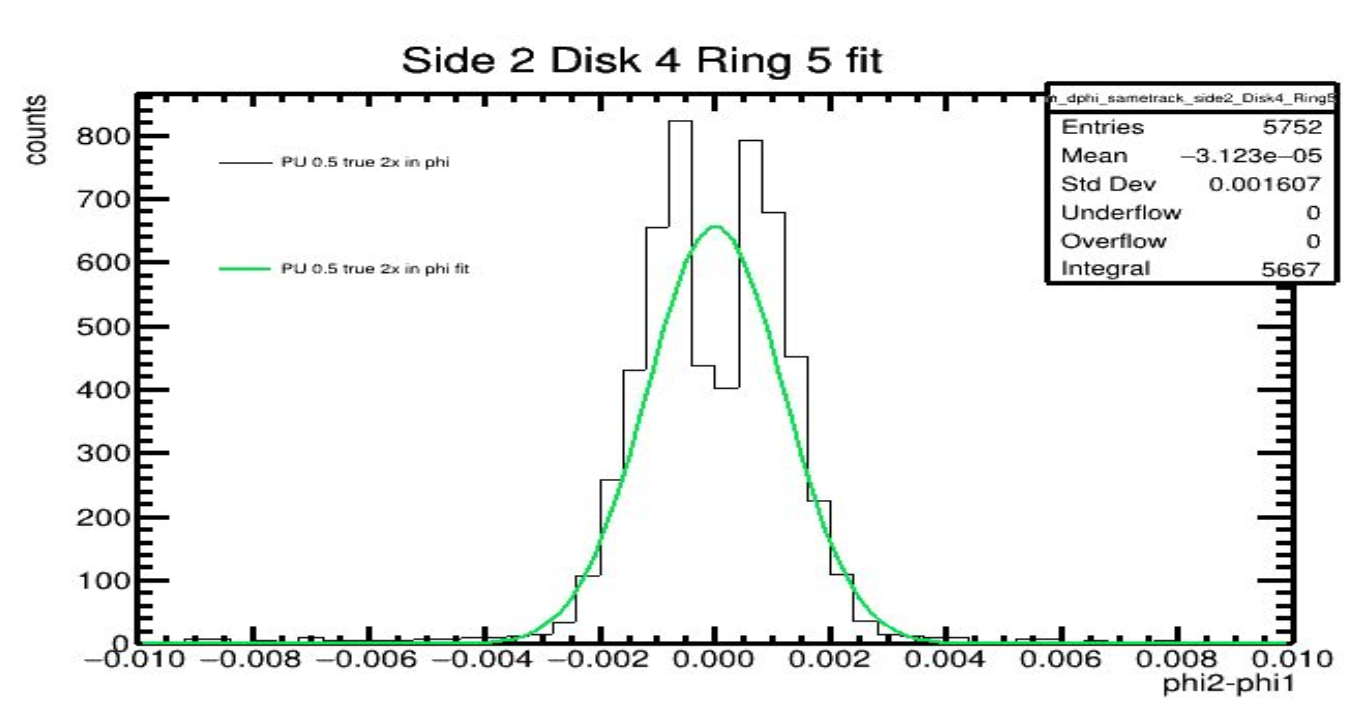
\includegraphics[width=1\textwidth]{ashish_thesis/D4R5_fit_PU0p5.png}
\caption[Fit Disk 4 Ring 5 (+Z) Cluster Distribution]{%
 Example fit using single Gaussian function of cluster count as a function of dphi variable for pileup 0.5 Disk 4 Ring 5 (+Z). 
}
\label{fig:cluster_ring_71}
\end{figure}

\end{comment}

%The mean of the fit is taken as the offset value and standard deviation is used as the selection on dr, dphi variables as shown in Table \ref{tab:disk_values}, \ref{tab:mdphi_cuts_values} and \ref{tab:mdr_cuts_offset_values}.

\begin{table}[H]
  \centering
  \caption[dr offset values for two-fold in phi]{dr mean values (mm) obtained from fit for two fold coincidences in phi for all disks and rings}
  \begin{tabular}{cccccc}
    \textbf{Disk} & \textbf{Ring 1} & \textbf{Ring 2} & \textbf{Ring 3} & \textbf{Ring 4} & \textbf{Ring 5} \\
    \hline
    %-1 & 0.0342041  & 0.0511416 & 0.0676943 & 0.0834355 & 0.0984932 \\
    %-2 & 0.0298276  & 0.0445398 & 0.0589828 & 0.0727454 & 0.0853587 \\
    %-3 & 0.0260326  & 0.0386608 & 0.05122   & 0.0632478 & 0.0746467 \\
    %-4 & 0.0227089  & 0.0336467 & 0.044476  & 0.0551065 & 0.06484   \\
    1  & 0.034  & 0.051 & 0.068 & 0.084 & 0.098 \\
    2  & 0.030  & 0.044 & 0.059 & 0.073 & 0.085 \\
    3  & 0.026  & 0.039 & 0.051 & 0.063 & 0.074 \\
    4  & 0.023   & 0.034 & 0.045 & 0.055 & 0.064 \\
  \end{tabular}
  \label{tab:mdr_cuts_offset_values}
\end{table}

\begin{table}[H]
  \centering
  \caption[dr cut values for two-fold in phi]{dr cut values (mm) for two fold coincidences in phi for all disks and rings}
  \begin{tabular}{cccccc}
    \textbf{Disk} & \textbf{Ring 1} & \textbf{Ring 2} & \textbf{Ring 3} & \textbf{Ring 4} & \textbf{Ring 5} \\
    \hline
    %-1 & 0.00633554 & 0.00709231 & 0.00757662 & 0.008659   & 0.00872148 \\
    %-2 & 0.00594206 & 0.00663493 & 0.00718173 & 0.00766371 & 0.00797059 \\
    %-3 & 0.00594206 & 0.00663493 & 0.00660603 & 0.00713035 & 0.00679445 \\
    %-4 & 0.00530235 & 0.00587692 & 0.00616465 & 0.00661972 & 0.00660599 \\
    1  & 0.0064 & 0.0072  & 0.0078 & 0.0086 & 0.0088 \\
    2  & 0.0059 & 0.0066 & 0.0070 & 0.0077 & 0.0079 \\
    3  & 0.0056 & 0.0062 & 0.0066 & 0.0070  & 0.0073 \\
    4  & 0.0053  & 0.0059 & 0.0061  & 0.0067 & 0.0068 \\
  \end{tabular}
  \label{tab:disk_values}
\end{table}

\begin{table}[H]
  \centering
  \caption[dphi cut values for two-fold in phi]{dphi cut values for two fold coincidences in phi for all disks and rings}
  \begin{tabular}{cccccc}
    \textbf{Disk} & \textbf{Ring 1} & \textbf{Ring 2} & \textbf{Ring 3} & \textbf{Ring 4} & \textbf{Ring 5} \\
    \hline
    %-1 & 0.000856727  & 0.00128078   & 0.00151297   & 0.00151297   & 0.0016561    \\
    %-2 & 0.000765842  & 0.00110698   & 0.00131104   & 0.00143555   & 0.00150265   \\
    %-3 & 0.000684645  & 0.000975385  & 0.00115899   & 0.00126858   & 0.00131598   \\
    %-4 & 0.000598839  & 0.000862728  & 0.00104327   & 0.00112621   & 0.00115609   \\
    1  & 0.00088  & 0.0013   & 0.0015    & 0.0016   & 0.0017   \\
    2  & 0.00076   & 0.0011   & 0.0013   & 0.0014   & 0.0015   \\
    3  & 0.00068  & 0.00097  & 0.0012   & 0.0013   & 0.0013   \\
    4  & 0.00061  & 0.00088  & 0.0010   & 0.0011   & 0.0012   \\
  \end{tabular}
  \label{tab:mdphi_cuts_values}
\end{table}


%A plot of two-fold coincidences in phi after applying all selection based on standard deviation values of all TEPX disks and rings is shown in Fig. \ref{fig:cluster_ring_720}.

\newpage
%\begin{figure}[H]
%\centering
%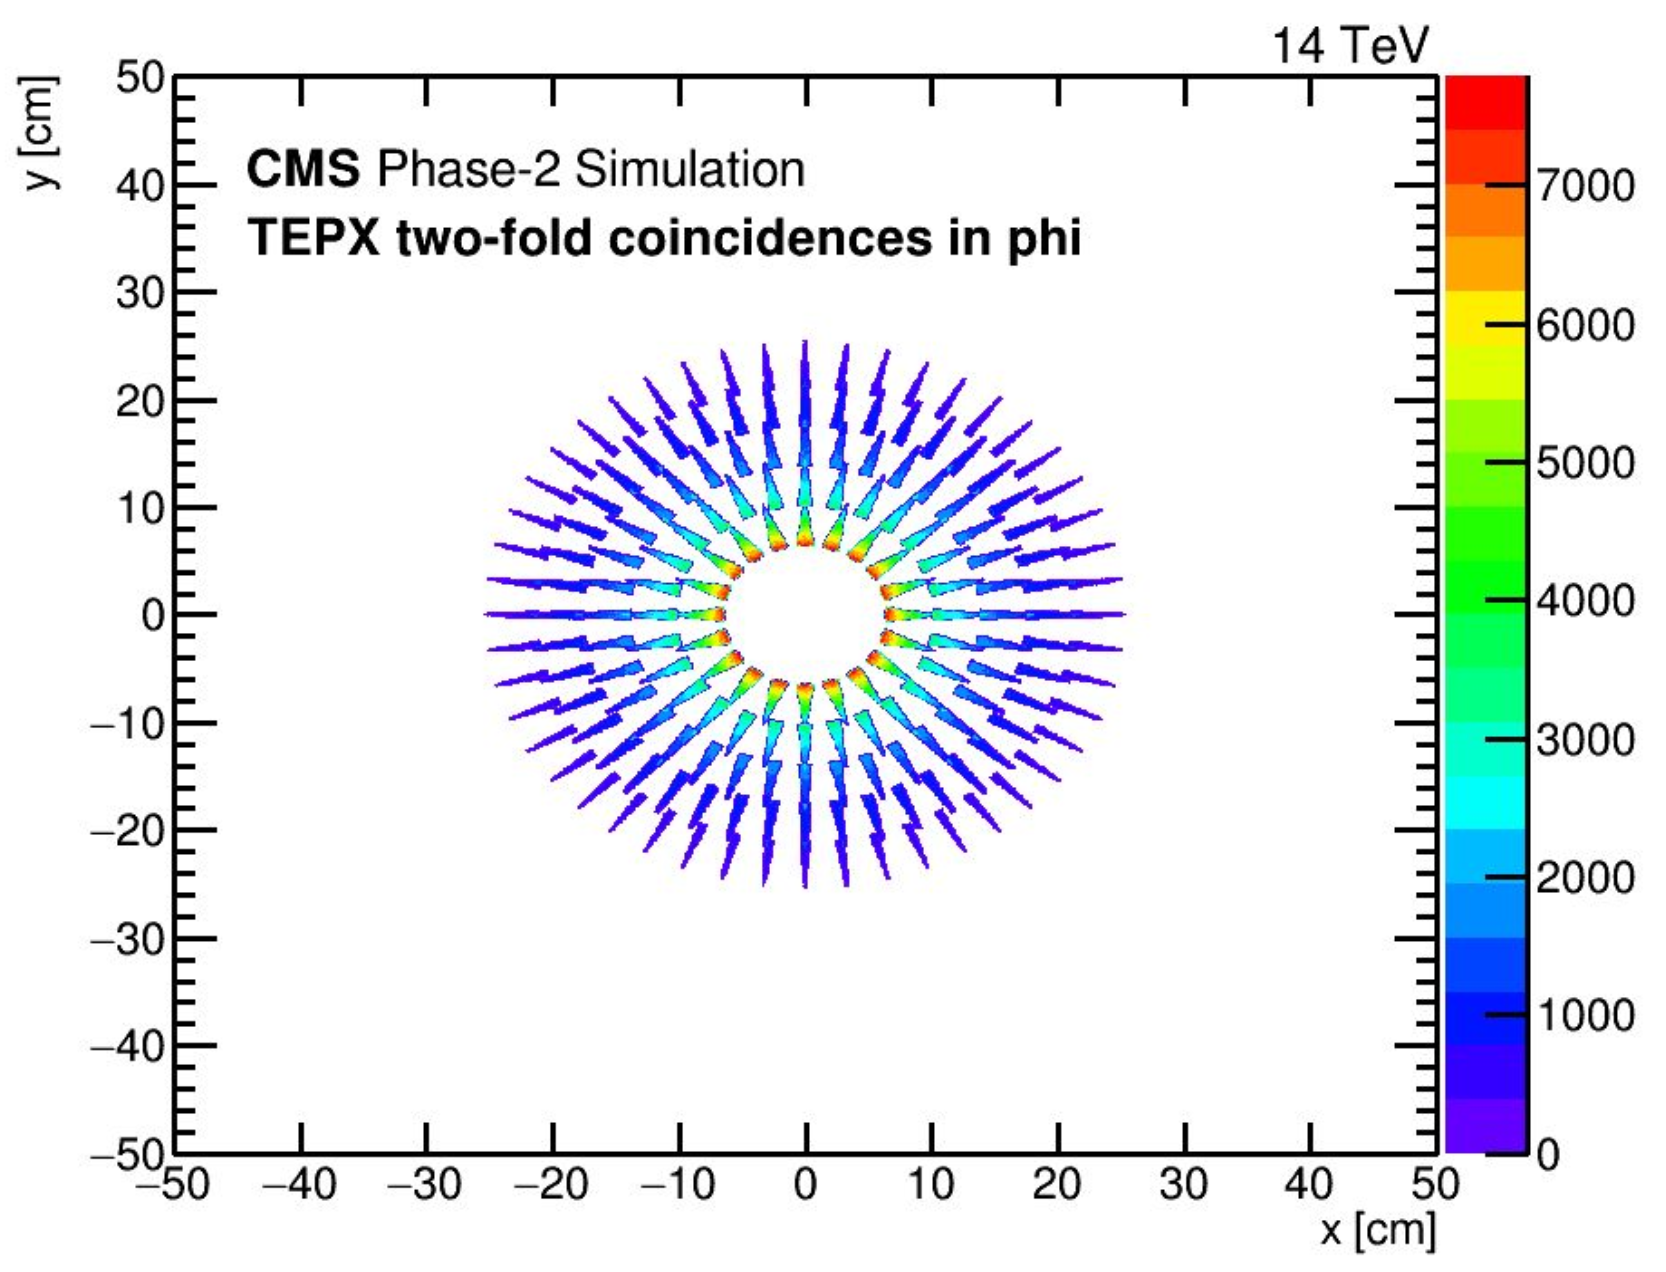
\includegraphics[width=0.6\textwidth]{ashish_thesis/twofoldinphi_sch.png}
%\caption[Map Of Two Fold Coincidences in phi]{%                                                                                                                                                       
 % Map of two fold coincidences in phi showing all module overlap regions.
%}
%\label{fig:cluster_ring_720}
%\end{figure}

Simlarly, we also studied two-fold coincidences in r which arise from module overlaps between successive rings by only considering one-to-one module overlap between first two and last two layers in one TEPX double-disk \cite{BRIL2021}.  %Table \ref{table:two_fold_coincidences} categorizes various types of two-fold coincidences in r, observed in the TEPX detector. These coincidences are labeled from A to L and arise due to the module overlap in different layers within a single TEPX double disk. The 'dz' column quantifies the spatial separation along beam axis between the coinciding layers,  the z coordinates for Layers L1 to L4 within the TEPX detector is also mentioned. These coordinates provide a precise location for each layer, contributing to the understanding of where these two fold coincidences are likely to occur. The two fold coincidence in r map showing module overlap regions for different types is shown in Fig. \ref{fig:cluster_ring_770}.
 A one-to-one overlapping of modules is considered between L1L2 and L3L4 modules as shown in Fig. \ref{fig:cluster_ring_72034}. %as shown in Fig. \ref{tab:my_label2}. 
 %The distributions for dr, dphi distribution depicting fake, true, total two fold coincidence in r for pileup 0.5 and 200 are shown in Fig. \ref{fig:cluster_ring_81} and \ref{fig:cluster_ring_82} respectively.
 Fit is done to pileup 0.5 distribution of true coincidences for both L1L2 and L3L4 coincidences in r. %as shown in Fig. \ref{fig:cluster_ring_83} and \ref{fig:cluster_ring_84}. 
  Fit results for all disks and rings are shown from  Table \ref{tab:my_label_55} to \ref{tab:my_label_54}. Similarly, two-sigma standard deviation selections are applied on dr, dphi variables. After applying all selections, the XY map of two-fold coincidences in r for L1L2 and L3L4 combined as shown in \ref{fig:cluster_ring_79}.

\begin{figure}[!htp]
\centering
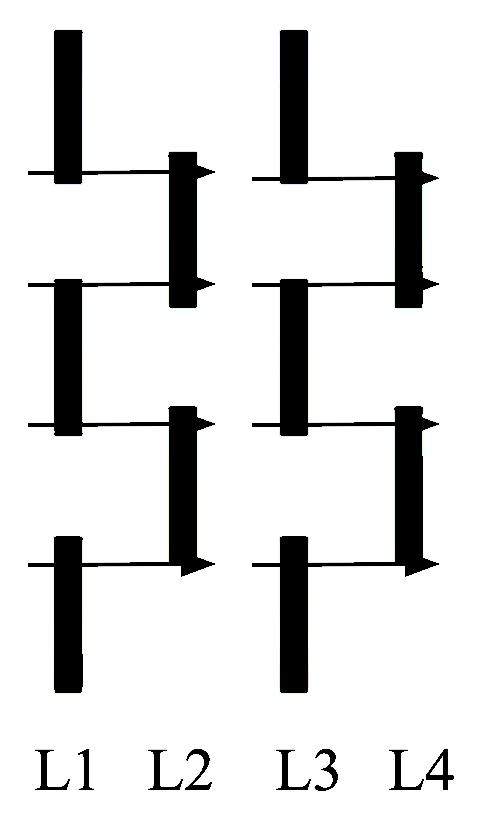
\includegraphics[width=0.3\textwidth]{ashish_thesis/twofoldinr_exam.png}
\caption[Examples of two fold coincidences in r]{%                                                                                                                                                       
  Definition of two-fold coincidences in r from the module overlap regions.
}
\label{fig:cluster_ring_72034}
\end{figure}


\begin{comment}

\begin{table}[H]
  \centering
  \caption[Two fold coincidences in r types]{Left: All type of two fold coincidences in r. Right: z coordinates for Layers L1 to L4.}
\begin{minipage}{0.45\textwidth}
    \centering
    \begin{tabular}{ccc}
    Modules & Type of Two Fold Coincidences & dz \\
    \hline
    A & R1L1-R2L2 & 0.4 \\
    B & R1L1-R2L4 & 1.2 \\
    C & R1L3-R2L4 & 0.4 \\
    D & R2L2-R3L3 & 0.4 \\
    E & R3L1-R2L2 & 0.4 \\
    F & R3L3-R2L4 & 0.4 \\
    G & R3L1-R4L2 & 0.4 \\
    H & R3L1-R4L4 & 1.2 \\
    I & R3L3-R4L4 & 0.4 \\
    J & R5L1-R4L2 & 0.4 \\
    K & R4L2-R5L3 & 0.4 \\
    L & R5L3-R4L4 & 0.4 \\
    \end{tabular}
\end{minipage}%
\hfill
\begin{minipage}{0.45\textwidth}
    \centering
    \begin{tabular}{cc}
    Layer & z-coordinate \\
    \hline
    Layer 1 (L1) & 264.4 \\
    Layer 2 (L2) & 264.8 \\
    Layer 3 (L3) & 265.2 \\
    Layer 4 (L4) & 265.6 \\
    \end{tabular}
\end{minipage}
\label{table:two_fold_coincidences}
\end{table}


\begin{figure}[!htp]
\centering
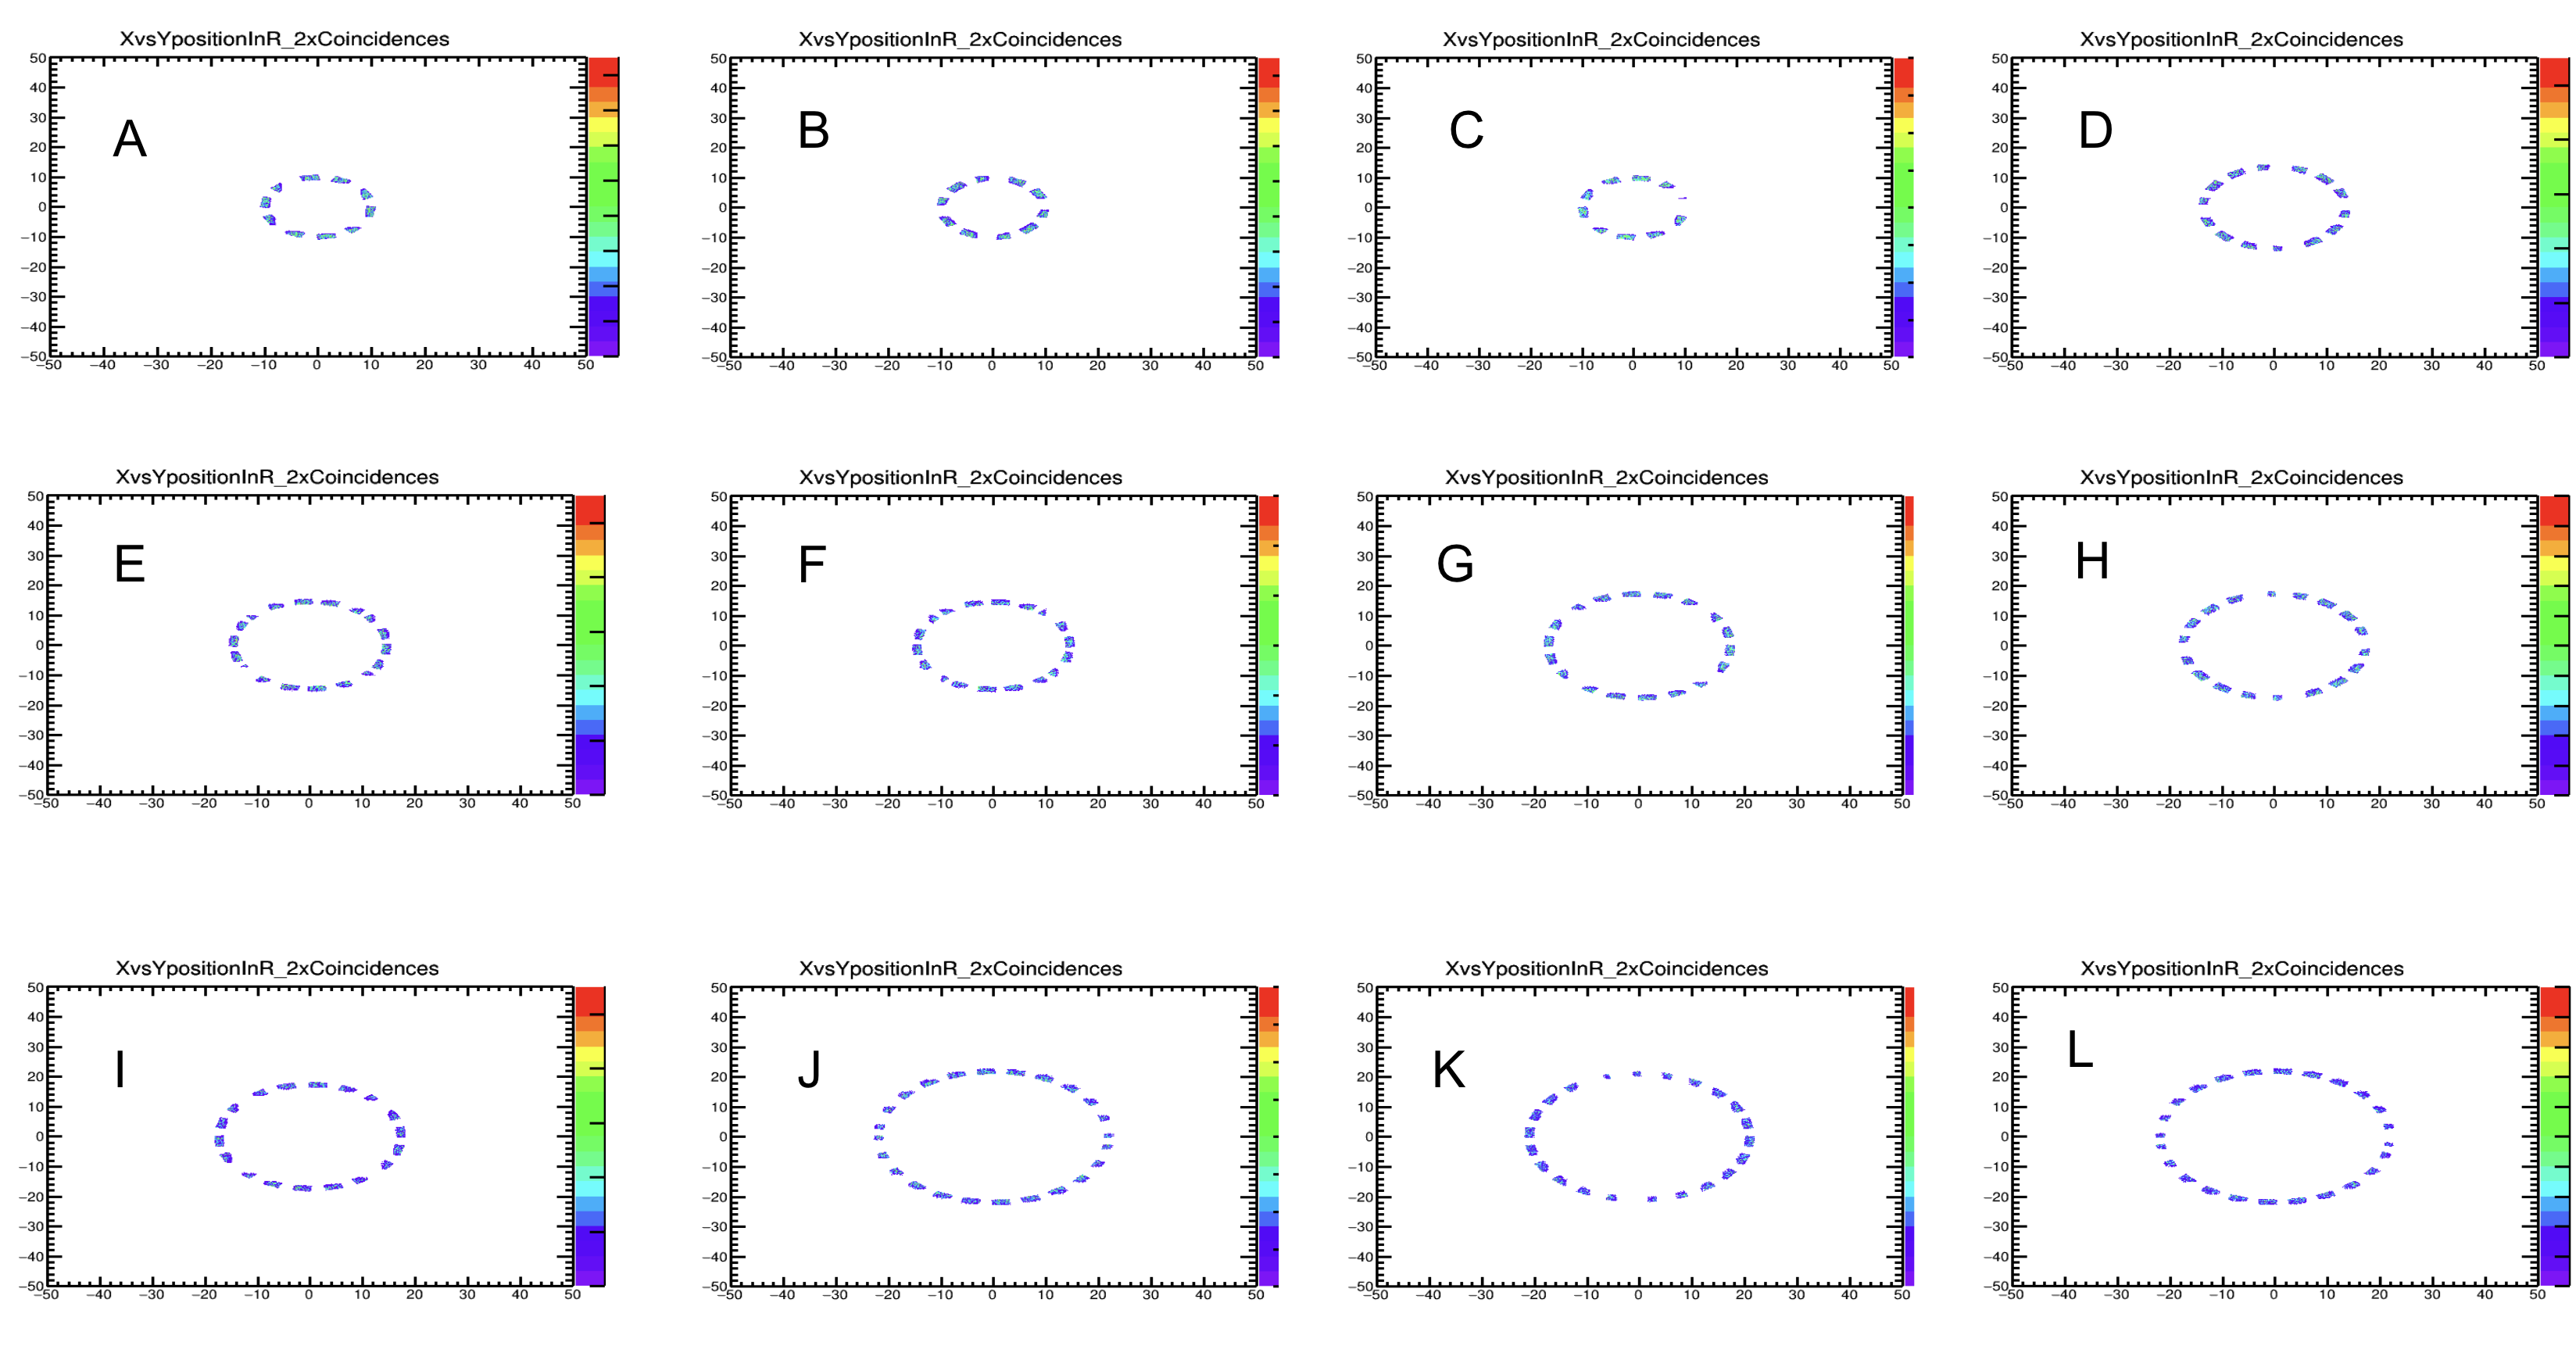
\includegraphics[width=1\textwidth]{ashish_thesis/twofoldinr_alltypes_diag.png}
\caption[Two Fold Coincidences in r types]{%                                                                                                                                                                                      
  Types of module overlap between different ring modules that can give rise to two fold coincidences in r.
}
\label{fig:cluster_ring_770}
\end{figure}

\begin{table}[H]
  \caption[Module mapping for two fold coincidenes in r]{Left: One to one module mapping in L1L2. Right: One to one module mapping in L3L4.}
  \begin{minipage}{0.45\linewidth}
    \centering
    %\caption{Left: One to one module mapping in L1L2. Right: One to one module mapping in L3L4}
    \begin{tabular}{cc}
      \textbf{R1L1} & \textbf{R2L2} \\
      \hline
      2 & 2 \\
      4 & 6 \\
      6 & 8 \\
      8 & 12 \\
      10 & 14 \\
      12 & 16 \\
      14 & 20 \\
      16 & 22 \\
      18 & 24 \\
      20 & 28 \\
    \end{tabular}
    %\label{tab:my_label1}
  \end{minipage}
  \hfill
  \begin{minipage}{0.45\linewidth}
    \centering
    %\caption{One to one module mapping in L3L4}
    \begin{tabular}{cc}
      \textbf{R1L3} & \textbf{R2L4} \\
      \hline
      1 & 1 \\
      3 & 5 \\
      5 & 7 \\
      7 & 9 \\
      9 & 13 \\
      11 & 15 \\
      13 & 19 \\
      15 & 21 \\
      17 & 23 \\
      19 & 27 \\
    \end{tabular}
    %\label{tab:my_label2}
  \end{minipage}
  \label{tab:my_label2}
\end{table}

\end{comment}

\begin{comment}

\begin{figure}[!htp]
\centering
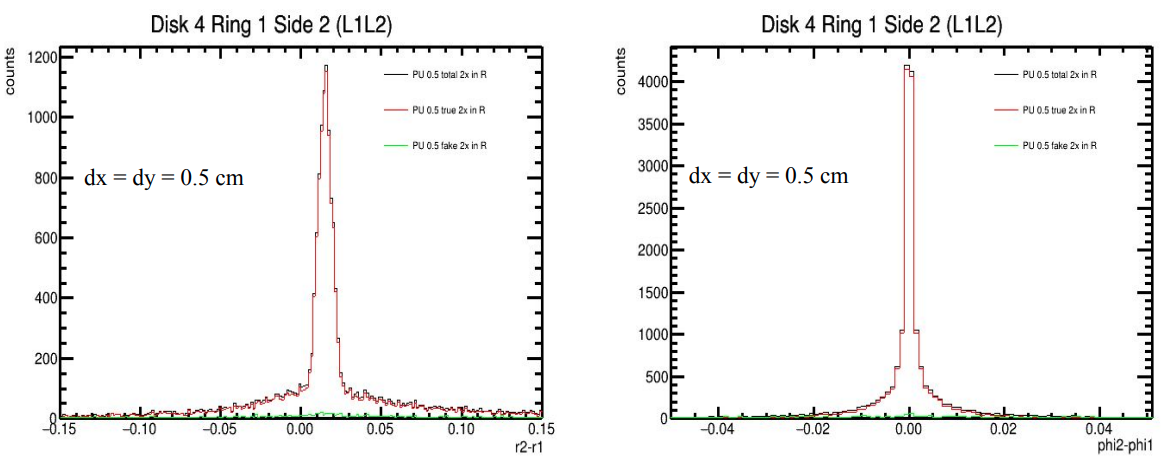
\includegraphics[width=1\textwidth]{ashish_thesis/l1l2_dr_dphi_D4R1S2.png}
\caption[D4R1 Two-Fold Coincidences vs. dr & dphi (PU 0.5)]{%
   PU 0.5 D4R1 total, true, fake two fold coincidences  in r as a function of dr, dphi variables.
}
\label{fig:cluster_ring_81}
\end{figure}

\begin{figure}[!htp]
\centering
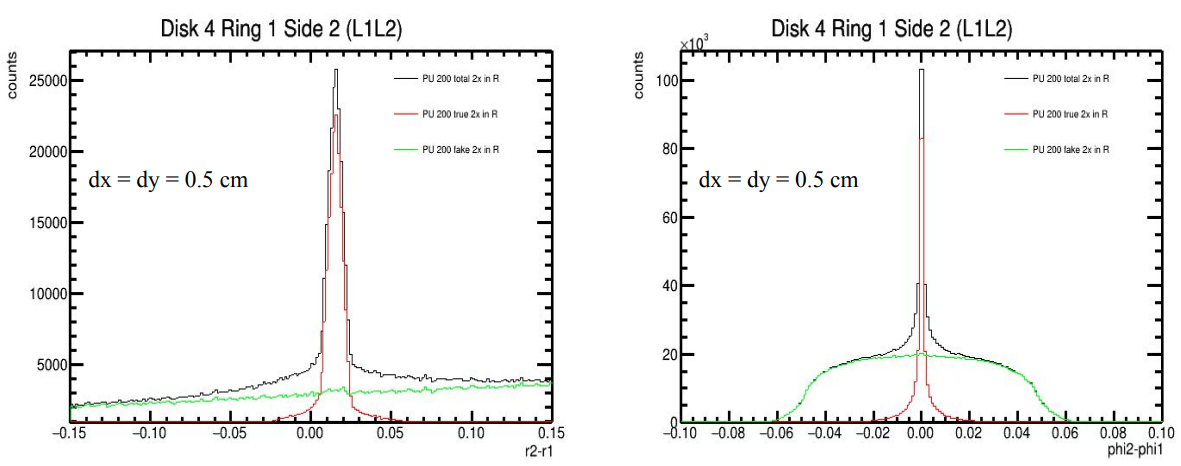
\includegraphics[width=1\textwidth]{ashish_thesis/l1l2_drdphi_2xinr_PU200.png}
\caption[D4R1 Two-Fold Coincidences vs. dr & dphi (PU 200)]{%
   PU 200 D4R1 total, true, fake two fold coincidences  in r as a function of dr, dphi variables.
}
\label{fig:cluster_ring_82}
\end{figure}

\endn{comment}

\begin{comment}

\begin{figure}[!htp]
\centering
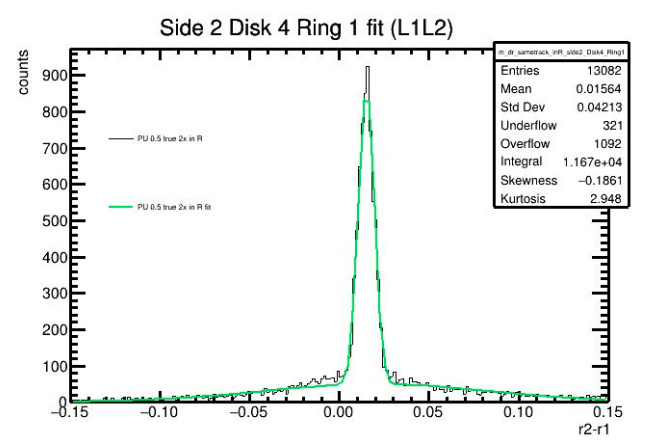
\includegraphics[width=1\textwidth]{ashish_thesis/fit_l1l2_dr_2xinr.png}
\caption[Fit L1L2 Two Fold Coincidences in r]{%
   Fit L1L2 two fold coincidences in R.
}
\label{fig:cluster_ring_83}
\end{figure}


\begin{table}[H]
  \centering
  \caption{Fit parameters for dr}
\begin{tabular}{ccc}
\textbf{Parameter Name} & \textbf{Value} & \textbf{Error} \\ 
\hline
p0 & 8.25e+02 & 1.40e+01 \\ 
p1 & 1.49e-02 & 6.52e-05 \\ 
p2 & 4.44e-03 & 5.61e-05 \\ 
p3 & 4.94e+01 & 1.18e+00 \\ 
p4 & 2.04e-02 & 9.87e-04 \\ 
p5 & 6.35e-02 & 1.14e-03 \\ 
\end{tabular}
\label{tab:my_label3}
\end{table}


\begin{figure}[!htp]
\centering
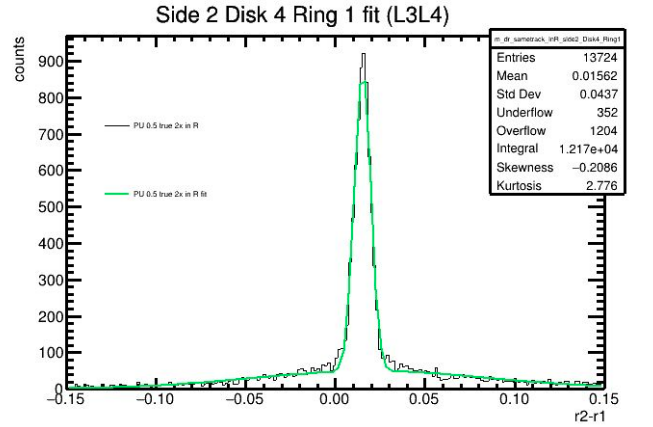
\includegraphics[width=1\textwidth]{ashish_thesis/fit_l3l4_dr_2xinr.png}
\caption[Fit L3L4 Two Fold Coincidences in r]{%
   Fit L3L4 two fold coincidences in r.
}
\label{fig:cluster_ring_84}
\end{figure}


\begin{table}[H]
  \centering
  \caption{Fit parameters for dr}
\begin{tabular}{ccc}
\textbf{Parameter Name} & \textbf{Value} & \textbf{Error} \\ 
\hline
p0 & 8.33e+02 & 1.43e+01 \\ 
p1 & 1.50e-02 & 6.56e-05  \\ 
p2 & 4.57e-03  & 6.01e-05 \\
p3 & 4.95e+01 & 1.17e+00 \\
p4 & 2.02e-02 & 1.04e-03  \\  
p5 & 6.68e-02 & 1.24e-03  \\ 
\end{tabular}
\label{tab:my_label6}
\end{table}

\end{comment}

%\begin{table}[h]
 % \centering
  %\caption{Fit parameters for dphi}
%\begin{tabular}{ccc}
%\textbf{Parameter Name} & \textbf{Value} & \textbf{Error} \\ 
%\hline
%p0 & 1.263e+03 & 2.52e+01 \\ 
%p1 & 0.00e+00 & fixed \\ 
%p2 & 4.510e-04 & 7.25e-06 \\
%\end{tabular}
%\label{tab:my_label10}
%\end{table}

\newpage
\begin{table}[H]
  \centering
  \caption[dr mean values for two-fold in r]{dr mean values (mm) obtained from fit to true coincidences in r}
\begin{tabular}{ccccc}
 & \multicolumn{4}{c}{\textbf{Ring}} \\
\textbf{Disk} & \textbf{1-2} & \textbf{2-3} & \textbf{3-4} & \textbf{4-5} \\
\hline
%-4 & 0.0230881 & 0.0309854 & 0.0387241 & 0.0464962 \\ 
%-3 & 0.0199761 & 0.0270206 & 0.0338467 & 0.0403068 \\ 
%-2 & 0.017385  & 0.0233397 & 0.0294101 & 0.0348779 \\ 
%-1 & 0.0150614 & 0.0202725 & 0.0255259 & 0.0303849 \\
1 & 0.023 & 0.031 & 0.039 & 0.047 \\
2 & 0.020 & 0.027 & 0.034 & 0.040 \\
3 & 0.018 & 0.023 & 0.029 & 0.035 \\
4 & 0.015 & 0.020  & 0.026 & 0.031 \\
\end{tabular}
\label{tab:my_label_55}
\end{table}


\begin{table}[H]
  \centering
  \caption[dr cut values for two-fold in r]{dr standard deviation (mm) values obtained from fit to true coincidences in r}
\begin{tabular}{ccccc}
 & \multicolumn{4}{c}{\textbf{Ring}} \\
\textbf{Disk} & \textbf{1-2} & \textbf{2-3} & \textbf{3-4} & \textbf{4-5} \\
\hline
%-4 & 0.00458531 & 0.00466448 & 0.00486059 & 0.0052905 \\ 
%-3 & 0.00444971 & 0.0046465 & 0.00472138 & 0.00490022 \\ 
%-2 & 0.00453556 & 0.00471864 & 0.00465781 & 0.00503102 \\ 
%-1 & 0.00457346 & 0.00458345 & 0.00478342 & 0.00497171 \\
1 & 0.0045 & 0.0045 & 0.0047 & 0.0052 \\
2 & 0.00442 & 0.0047 & 0.0048 & 0.0050 \\
3 & 0.0045 & 0.0045 & 0.0049 & 0.0049 \\
4 & 0.0045 & 0.0047 & 0.0049 & 0.0049 \\
\end{tabular}
\label{tab:my_label_53}
\end{table}



\begin{table}[H]
  \centering
  \caption[dphi cut values for two-fold in r]{dphi standard deviation values obtained from fit to true coincidences in r}
\begin{tabular}{ccccc}
 & \multicolumn{4}{c}{\textbf{Ring}} \\
\textbf{Disk} & \textbf{1-2} & \textbf{2-3} & \textbf{3-4} & \textbf{4-5} \\
\hline
%-4 & 0.000628313 & 0.000828659 & 0.000975585 & 0.00101984 \\ 
%-3 & 0.000545699 & 0.000722289 & 0.00081899 & 0.000918094 \\ 
%-2 & 0.000495422 & 0.000649127 & 0.000754224 & 0.000839347 \\ 
%-1 & 0.000451069 & 0.000604104 & 0.000689508 & 0.000755603 \\
1 & 0.00063 & 0.00082 & 0.00094 & 0.0010 \\
2 & 0.00057 & 0.00076 & 0.00085 & 0.00090 \\
3 & 0.00052 & 0.00066 & 0.00077 & 0.00083 \\
4 & 0.00047 & 0.00059 & 0.00069 & 0.00075 \\
\end{tabular}
\label{tab:my_label_54}
\end{table}



\begin{comment}

\begin{table}[H]
  \centering
  \caption[dphi cut values (L3L4)]{dphi standard deviation values obtained from fit for all disks and rings for coincidences in r in layers L3L4}
\begin{tabular}{ccccc}
 & \multicolumn{4}{c}{\textbf{Ring}} \\
\textbf{Disk} & \textbf{1} & \textbf{2} & \textbf{3} & \textbf{4} \\
\hline
%-4 & 0.00448255 & 0.00445856 & 0.00474102 & 0.0051553 \\ 
%-3 & 0.00442349 & 0.00472485 & 0.00474663 & 0.0050426 \\ 
%-2 & 0.00450002 & 0.0045179 & 0.00492058 & 0.00494887 \\ 
%-1 & 0.00444657 & 0.00468584 & 0.00493828 & 0.00488064 \\
1 & 0.00458531 & 0.00466448 & 0.00486059 & 0.0052905 \\
2 & 0.00444971 & 0.0046465 & 0.00472138 & 0.00490022 \\
3 & 0.00453556 & 0.00471864 & 0.00465781 & 0.00503102 \\
4 & 0.00457346 & 0.00458345 & 0.00478342 & 0.00497171 \\
\end{tabular}
\label{tab:my_label_52}
\end{table}



\begin{table}[H]
  \centering
  \caption[dphi cut values (L3L4)]{dphi standard deviation values obtained from fit for all disks and rings for coincidences in r in layers L3L4}
\begin{tabular}{ccccc}
 & \multicolumn{4}{c}{\textbf{Ring}} \\
\textbf{Disk} & \textbf{1} & \textbf{2} & \textbf{3} & \textbf{4} \\
\hline
%-4 & 0.000627781 & 0.000814669 & 0.000941641 & 0.0010221 \\ 
%-3 & 0.000573352 & 0.000761853 & 0.000851161 & 0.000901014 \\ 
%-2 & 0.000523361 & 0.000662691 & 0.000778358 & 0.000834924 \\ 
%-1 & 0.000471669 & 0.000589938 & 0.000692007 & 0.000750302 \\
1 & 0.000628313 & 0.000828659 & 0.000975585 & 0.00101984 \\
2 & 0.000545699 & 0.000722289 & 0.00081899 & 0.000918094 \\
3 & 0.000495422 & 0.000649127 & 0.000754224 & 0.000839347 \\
4 & 0.000451069 & 0.000604104 & 0.000689508 & 0.000755603 \\
\end{tabular}
\label{tab:my_label_51}
\end{table}


\begin{table}[H]
  \centering
  \caption[dr mean values (L3L4)]{dr mean values obtained from fit for all disks and rings for coincidences in r in layers L3L4}
\begin{tabular}{ccccc}
 & \multicolumn{4}{c}{\textbf{Ring}} \\
\textbf{Disk} & \textbf{1} & \textbf{2} & \textbf{3} & \textbf{4} \\
\hline
%-4 & 0.0229736 & 0.0311421 & 0.0390871 & 0.0468038 \\ 
%-3 & 0.0202136 & 0.0268963 & 0.0337796 & 0.040398 \\ 
%-2 & 0.0174894 & 0.0233893 & 0.0293971 & 0.0351501 \\ 
%-1 & 0.0149661 & 0.020194 & 0.0255051 & 0.0305483 \\
1 & 0.0230881 & 0.0309854 & 0.0387241 & 0.0464962 \\
2 & 0.0199761 & 0.0270206 & 0.0338467 & 0.0403068 \\
3 & 0.017385 & 0.0233397 & 0.0294101 & 0.0348779 \\
4 & 0.0150614 & 0.0202725 & 0.0255259 & 0.0303849 \\
\end{tabular}
\label{tab:my_label_50}
\end{table}

\end{comment}


\begin{comment}

\begin{figure}[!htp]
\centering
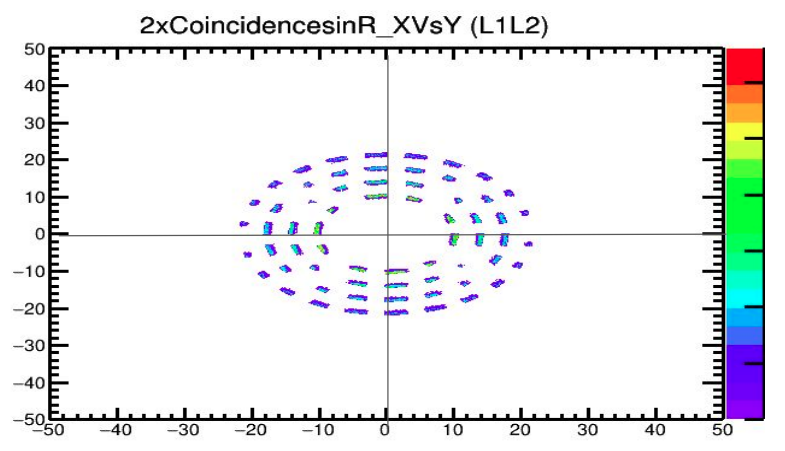
\includegraphics[width=1\textwidth]{ashish_thesis/l1l2_2xinr.png}
\caption[L1L2 Module Overlap Map for Two Fold Coincidences in r]{%                                                                                                                                   
   Module overlap map in L1L2 layers for two fold coincidences in r.
}
\label{fig:cluster_ring_77}
\end{figure}

\begin{figure}[!htp]
\centering
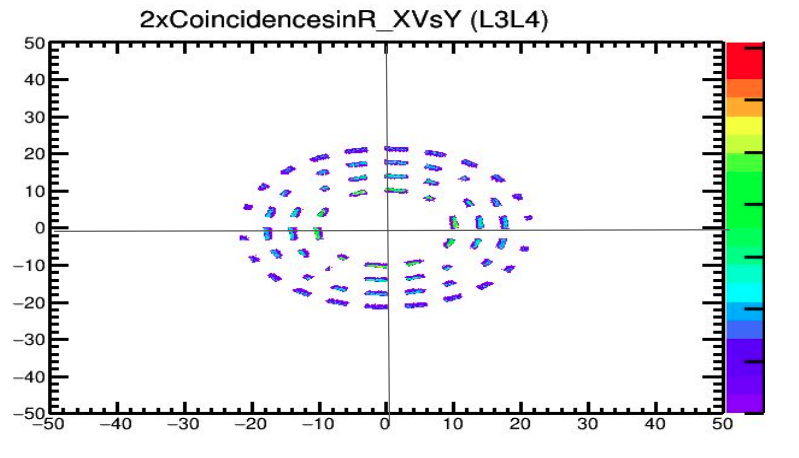
\includegraphics[width=1\textwidth]{ashish_thesis/l3l4_2xinr.png}
\caption[L3L4 Module Overlap Map for Two Fold Coincidences in r]{%                                                                                                                                                        
   Module overlap map in L3L4 layers for two fold coincidences in r.
}
\label{fig:cluster_ring_78}
\end{figure}

\end{comment}

\newpage

\begin{figure}[H]
\centering
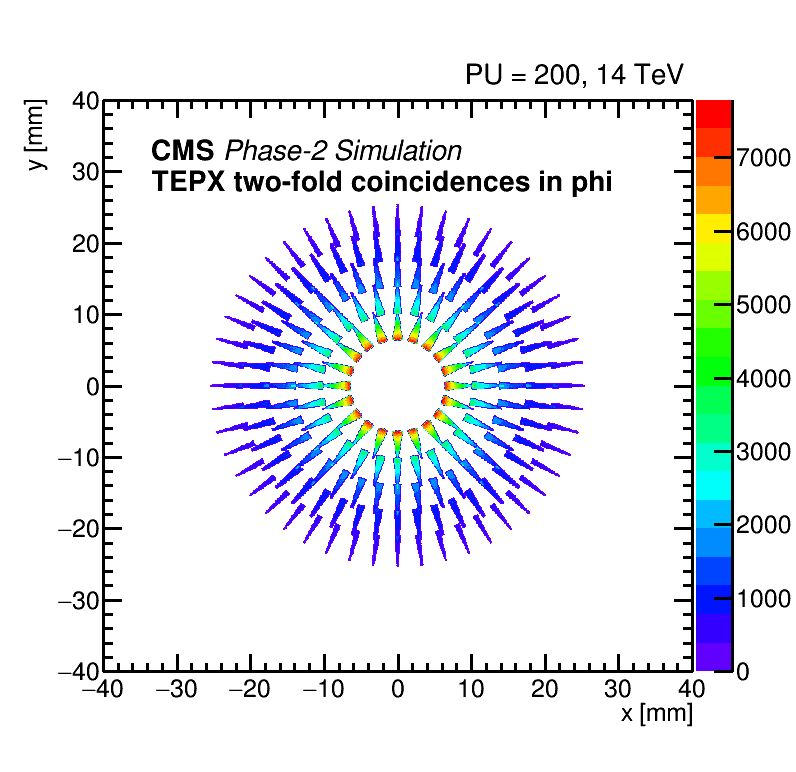
\includegraphics[width=0.6\textwidth]{ashish_thesis/twofoldinphi_sch_1.png}
\caption[Map Of Two Fold Coincidences in phi]{%                                                                                                            
   X-Y map of reconstructed two-fold coincidences in $\phi$ showing module overlap regions.
}
\label{fig:cluster_ring_720}
\end{figure}


\begin{figure}[H]
\centering
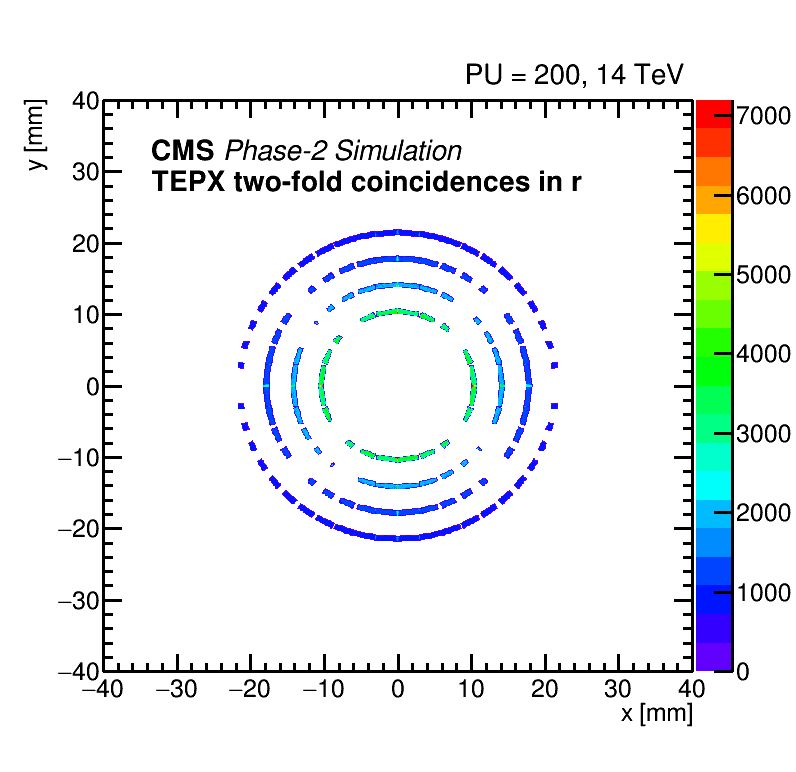
\includegraphics[width=0.6\textwidth]{ashish_thesis/l1l2_l3l4_2xinr_2.png}
\caption[L1L2 and L3L4 Module Overlap Map for Two Fold Coincidences in r]{%                                                                                                                                                                                      
   X-Y map of reconstructed two-fold coincidences in r using the selections described in the text. We have only reconstructed coincidences in r arising from module overlap in L1L2 and L3L4. The gaps in the plot correspond to other types of two fold coincidences in r that will arise from module overlap in L1L4, L3L4 and L2L3.
}
\label{fig:cluster_ring_79}
\end{figure}

\newpage
The new algorithm is able to remove physics noise at high pileup as can be seen from the high efficiency values and low fake rates for Disk 4 all rings and all pileup samples as shown in Table  \ref{tab:sample} and \ref{tab:combined_sample}. The fake two-fold coincidence rates for different rings in Disk 4 with a pileup of 200 are presented. The rate changes across the rings, starting from 1.1 \% in Ring 1 and increasing to 2.5 \% in Ring 4, before slightly decreasing to 2.3 \% in Ring 5. This variation suggests that the fake coincidences is not uniform across the rings of Disk 4, with the middle rings (Rings 3 and 4) showing a higher fake rate. There is a general trend of increasing fake rates with pileup. For instance, at a pileup of 0.5, the fake rates for "2-fold in phi" and "2-fold in r" are 0.78\% and 0.99\%, respectively. These rates gradually increase as the pileup value rises, reaching 1.85\% for "two-fold in phi" and 1.57\% for "two-fold in r" at a pileup of 200. Fake rate is defined as\begin{equation}
\text{Fake rate} = \frac{\text{Number of fake coincidences (Area under the green curve)}}{\text{Total number of coincidences (Area under the black curve)}}
\end{equation} as shown in Fig. 1.9.

\begin{table}[H]
  \centering
  \caption{Fake rate for Disk 4 for pileup 200}
  \begin{tabular}{cc}
    \textbf{Disk 4} & \textbf{Fake two-fold coincidence rate (\%)} \\
    \hline
    Ring 1 &  1.1\\
    Ring 2 &  1.9\\
    Ring 3 &  2.0\\
    Ring 4 &  2.5\\
    Ring 5 &  2.3\\
  \end{tabular}
  \label{tab:sample}
\end{table}

\begin{comment}
  
\begin{table}[H]
  \centering
  \caption{TEPX two-fold coincidences fake rate and efficiency}
  \begin{tabular}{ccccc}
    \textbf{Pileup} & \textbf{Fake rate 2-fold in phi (\%)} & \textbf{Fake rate 2-fold in r (\%)} & \textbf{Efficiency 2-fold in phi (\%)} & \textbf{Efficiency 2-fold in r (\%)} \\
    \hline
    0.5  & 0.78 & 0.99 & 99.21 & 99.00 \\
    1    & 0.79 & 1.01 & 99.20 & 98.98 \\
    1.5  & 0.80 & 1.02 & 99.19 & 98.97 \\
    2    & 0.79 & 1.02 & 99.20 & 98.97 \\
    10   & 0.83 & 1.04 & 99.16 & 98.95 \\
    30   & 0.94 & 1.09 & 99.05 & 98.90 \\
    50   & 1.04 & 1.14 & 98.95 & 98.85 \\
    100  & 1.31 & 1.29 & 98.68 & 98.70 \\
    140  & 1.53 & 1.41 & 98.46 & 98.58 \\
    200  & 1.85 & 1.57 & 98.14 & 98.42 \\
  \end{tabular}
  \label{tab:combined_sample}
\end{table}

\end{comment}
  
\begin{table}[H]
  \centering
  \caption{TEPX two-fold coincidences fake rate and efficiency}
  \begin{tabular}{ccccc}
    & \multicolumn{2}{c}{\textbf{Fake rate (\%)}} & \multicolumn{2}{c}{\textbf{Efficiency (\%)}} \\
    %\cline{2-5}
    \textbf{Pileup}  & \textbf{2-fold in phi} & \textbf{2-fold in r} & \textbf{2-fold in phi} & \textbf{2-fold in r} \\
    \hline
    0.5  & 0.78 & 0.99 & 99.21 & 99.00 \\
    1    & 0.79 & 1.01 & 99.20 & 98.98 \\
    1.5  & 0.80 & 1.02 & 99.19 & 98.97 \\
    2    & 0.79 & 1.02 & 99.20 & 98.97 \\
    10   & 0.83 & 1.04 & 99.16 & 98.95 \\
    30   & 0.94 & 1.09 & 99.05 & 98.90 \\
    50   & 1.04 & 1.14 & 98.95 & 98.85 \\
    100  & 1.31 & 1.29 & 98.68 & 98.70 \\
    140  & 1.53 & 1.41 & 98.46 & 98.58 \\
    200  & 1.85 & 1.57 & 98.14 & 98.42 \\
  \end{tabular}
  \label{tab:combined_sample}
\end{table}




\begin{comment}

\begin{table}[H]
  \centering
  \caption{TEPX two fold coincidences fake rate}
\begin{tabular}{cccc}
\textbf{Pileup} & \textbf{Fake two fold} & \textbf{Fake two fold} & \textbf{Fake two} \\
\textbf{} & \textbf{coincidence in phi} & \textbf{coincidence in R} & \textbf{fold coincidence} \\
\hline
0.5  &  0.78& 0.99 & 0.83 \\
1& 0.79 &  1.01 &0.85\\
1.5 &  0.80& 1.02 & 0.86 \\
2 & 0.79 & 1.02&  0.84\\
10 &  0.83&  1.04&  0.88\\
30&  0.94&  1.09&  0.98\\
50 &  1.04&  1.14&  1.07\\
100  & 1.31 & 1.29& 1.31\\
140  & 1.53 & 1.41& 1.50\\
200   & 1.85 & 1.57 &1.78\\
\end{tabular}
\label{tab:sample_1}
\end{table}


\begin{table}[H]
  \centering
  \caption{TEPX two coincidences efficiency}
\begin{tabular}{cccc}
\textbf{Pileup} & \textbf{Efficiency for two} & \textbf{Efficiency for Fake} & \textbf{Efficiency for two} \\
& \textbf{fold coincidence in phi} & \textbf{two fold coincidence in R} & \textbf{fold coincidence} \\
\hline
0.5  & 99.21 &99.00  &99.16  \\
1& 99.20 &98.98  & 99.14 \\
1.5 & 99.19 & 98.97 & 99.13 \\
2& 99.20 & 98.97 & 99.13 \\
10 & 99.16 & 98.95 & 99.11 \\
30& 99.05 & 98.90 & 99.01 \\
50 & 98.95 & 98.85 & 98.92 \\
100& 98.68 & 98.70 & 98.68 \\
140& 98.46 & 98.58 & 98.49 \\
200 &98.14  & 98.42 &98.21  \\
\end{tabular}
\label{tab:sample_2}
\end{table}

\end{comment}

%Ratio of the integrals for fake & total coincidence for dr & dphi distributions is 3454/145988 = 0.023

We study the linearity of two-fold coincidences that is how the number of two-fold coincidences change with pileup to obtain precise luminosity measurement \cite{sehrawat2022optimisation}. Distribution of two-fold coincidences for TEPX Disk 4 Ring 1 for all pileup values is shown in Fig. \ref{fig:tepx_coin_allPU}. For pileup 200, mean two-fold coincidences is around 270. The new algorithm is able to suppress non-linearity at high pileup values as shown in Fig.  \ref{fig:CMS_420}  and \ref{fig:CMS_4207}. Non-linearity is within 1 \% for entire pileup range.

\begin{figure}[H]
  \centering
  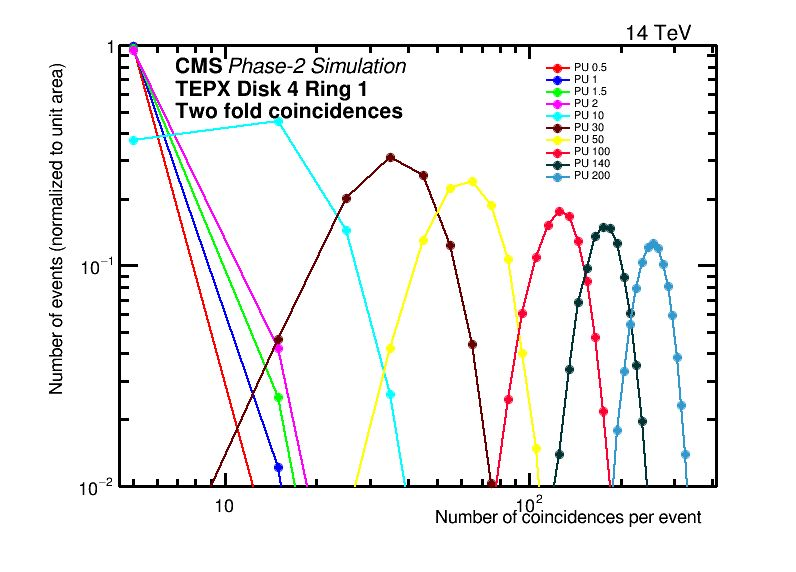
\includegraphics[width=0.7\columnwidth]{ashish_thesis/tepx_D4R1_coin_allpu_1.png}
  \caption[TEPX D4R1 Two-Fold Coincidences All Pileup]{Distribution of number of two-fold coincidences for TEPX Disk 4 Ring 1 for all pileup values.}
  \label{fig:tepx_coin_allPU}
\end{figure}


\begin{figure}[H]
  \centering
  \includegraphics[width=1\columnwidth]{ashish_thesis/michigan_1.png}
  \caption[TEPX two-fold coincidences linear fit per disk]{\onehalfspacing Left: Simulated mean number of two-fold coincidences for TEPX disks as a function of pileup. A line is fitted between pileup values of 0 and 2, and then extrapolated up to a pileup of 200. Right: The relative difference between the data points and the values of the fit function at the respective pileup value.}
  \label{fig:CMS_420}
\end{figure}


\begin{figure}[H]
  \centering
  \includegraphics[width=1\columnwidth]{ashish_thesis/michigan_4.png}
  \caption[TEPX two-fold coincidences linear fit for Disk 4 Ring 1]{\onehalfspacing Left: Simulated mean number of two-fold coincidences in phi for TEPX Disk 4 Ring 1 as a function of pileup. A line is fitted between pileup values of 0 and 2, and then extrapolated up to a pileup of 200. Right: The relative difference between the data points and the values of the fit function at the respective pileup value.}
  \label{fig:CMS_4207}
\end{figure}



\begin{comment}

\begin{figure}[H]
  \centering
  \includegraphics[width=1 \columnwidth]{ashish_thesis/totalcoincidences.png}
  \caption[TEPX Two Fold Coincidences Fit And Residual]{Left: Simulated mean number of coincidences in $\phi$ and r for all entire TEPX detector as a function of pileup. A line is fitted between pileup values of 0 and 2, and then extrapolated up to a pileup of 200. Right: Deviation from linearity for coincidence in $\phi$ and r for entire TEPX detector. The non-linearity is calculated as the relative difference between the data points and the values of the fit function at the respective pileup value. Non-linearity is within 1 \% for entire pileup range. Pileup 200 corresponds to High Luminosity (HL)-LHC environment.}
  \label{fig:CMS}
\end{figure}


\begin{figure}[H]
  \centering
  \includegraphics[width=1\columnwidth]{ashish_thesis/totalcoincidencesD4R1.png}
  \caption[Two Fold Coincidences for Disk 4 Ring 1 Fit And Residual]{Left: Simulated mean number of coincidences in $\phi$ and r for TEPX Disk 4 Ring 1 as a function of pileup. Right: Deviation from linearity for coincidences in $\phi$ and r for TEPX Disk 4 Ring 1. The non-linearity is calculated as the relative difference between the data points and the values of the fit function at the respective pileup value.}
  \label{fig:CMS}
\end{figure}


\begin{figure}[H]
  \centering
  \includegraphics[width=1\columnwidth]{ashish_thesis/coincidencesperdisk+z.png}
  \caption[Two Fold Coincidences Per Disk Fit And Residual]{Left: Simulated mean number of coincidences in $\phi$ and r for +z side TEPX disks as a function of pileup. Right: Deviation from linearity for coincidences in $\phi$ and r for +z side TEPX disks.}
  \label{fig:CMS}
\end{figure}


\begin{figure}[H]
  \centering
  \includegraphics[width=1\columnwidth]{ashish_thesis/coincidencesinphiD4R1z+.png}
  \caption[Two Fold Coincidences in phi for Disk 4 Ring 1 Fit And Residual]{Left: Simulated mean number of coincidences in $\phi$ for TEPX +z side Disk 4 Ring 1 as a function of pileup. Right: Deviation from linearity for coincidences in $\phi$ for TEPX +z side Disk 4 Ring 1. The non-linearity is calculated as the relative difference between the data points and the values of the fit function at the respective pileup value.}
  \label{fig:CMS}
\end{figure}



\begin{figure}[H]
  \centering
  \includegraphics[width=1\columnwidth]{ashish_thesis/coincidencesinphiperringD+4.png}
  \caption[Two fold coincidences in phi per ring Fit And Residual]{Left: Simulated mean number of coincidences in $\phi$ for +z side TEPX Disk 4 per ring as a function of pileup. Ring 1 has highest slope and Ring 5 has least slope. Right: Deviation from linearity for coincidences in $\phi$ for +z side TEPX Disk 4 per ring. Non-linearity is within 1\% for all rings over entire pileup range.}
  \label{fig:CMS}
\end{figure}


\begin{figure}[H]
  \centering
  \includegraphics[width=1\columnwidth]{ashish_thesis/coincidencesinrperringD+4.png}
  \caption[Two Fold Coincidences in r Per Ring Fit And Residual]{Left: Simulated mean number of coincidences in r for +z side TEPX Disk 4 per ring as a function of pileup. Ring 1 has highest slope and Ring 5 has least slope. Right: Deviation from linearity for coincidences in r for +z side TEPX Disk 4 per ring. Non-linearity is within $1\%$ for all rings over entire pileup range.}
  \label{fig:CMS_999}
\end{figure}

\end{comment}

\begin{comment}
  
For Disk 4 Ring 1, fake coincidences are randomly distributed and true coincidences are localized in the middle of the distribution as shown in Fig. \ref{fig:cluster_ring_20}.  For Disk 4 Ring 5, fake coincidence are randomly distributed. True coincidences are localized in the middle of the distribution. Compared to Ring 1, there are less true coincidences in the middle part of the distribution as shown in Fig. \ref{fig:cluster_ring_21}.


\begin{figure}[!htp]
  \centering
  \includegraphics[width=1\columnwidth]{ashish_thesis/coincidencesinrD4R1z+.png}
  \caption[Two Fold Coincidences in r Disk 4 Ring 1 Fit And Residual]{Left: Simulated mean number of coincidences in r for TEPX +z side Disk 4 Ring 1 as a function of pileup. Right: Deviation from linearity for coincidences in r for TEPX +z side Disk 4 Ring 1. The non-linearity is calculated as the relative difference between the data points and the values of the fit function at the respective pileup value.}
  \label{fig:CMS}
\end{figure}


\begin{figure}[H]
  \centering
  \includegraphics[width=1\columnwidth]{ashish_thesis/coincidencesperringD+4.png}
  \caption[Two fold coincidences per ring Fit And Residual]{Left: Simulated mean number of coincidences in $\phi$ and r for +z side TEPX Disk 4 per ring as a function of pileup. Ring 1 has highest slope and Ring 5 has least slope. Right: Deviation from linearity for coincidences in $\phi$ and r for +z side TEPX Disk 4 per ring. Non-linearity is within 1\% for all rings over entire pileup range.}
  \label{fig:CMS}
\end{figure}

\centering
\includegraphics[width=1\textwidth]{ashish_thesis/D4R1_fake_true_ratio.png}
\caption[Disk 4 Ring 1 Fake/Total coincidences]{%
  Ratio of fake and total two fold coincidences for disk 4 ring 1.
}
\label{fig:cluster_ring_20}
\end{figure}


\begin{figure}[!htp]
\centering
\includegraphics[width=1\textwidth]{ashish_thesis/D4R5_fake_true_ratio.png}
\caption[Disk 4 Ring 5 Fake/Total coincidences]{%
  Ratio of fake and total two fold coincidences for disk 4 ring 5.
}
\label{fig:cluster_ring_21}
\end{figure}

\end{comment}

\subsection{TEPX three-fold coincidences}

It is possible to have three fold coincidences in TEPX detector. A three-fold coincidence refers to a situation where three hits occur in a close spatial arrangement originating from the same underlying event. In the current algorithm, we look for another cluster in the lower ring after a two fold coincidence cluster in phi is found. The selections used for finding three-fold coincidences using old dx, dy and dz cut variables are 0.1 mm, 0.1 mm and 0.9 mm. The XY map of three-fold coincidences is shown in Fig. \ref{fig:tepx_3foldcoin_allPU_1}. Three-fold coincidences under all pileup conditions is shown in Fig.  \ref{fig:tepx_3foldcoin_allPU_2}.  With the current algorithm, three-fold coincidences shows non-linearity as shown in Fig. \ref{fig:tepx_3foldcoin_allPU_3}. % and Fig.  \ref{fig:tepx_3foldcoin_lowPU}.

\begin{figure}[H]
  \centering
  \includegraphics[width=0.8\columnwidth]{ashish_thesis/tepx_threefold_coincidences_1.png}
  \caption[Regions in XY plane showing three-fold coincidences]{Reconstructed three fold coincidences in all rings within TEPX double-disk.}
  \label{fig:tepx_3foldcoin_allPU_1}
\end{figure}

\newpage
\begin{figure}[H]
  \centering
  \includegraphics[width=0.7\columnwidth]{ashish_thesis/tepx_threefold_allpu.png}
  \caption[TEPX Disk 4 Ring 2 Three Fold Coincidences]{Distribution of number of three fold coincidences for TEPX Disk 4 Ring 2 for all pileup values.}
  \label{fig:tepx_3foldcoin_allPU_2}
\end{figure}

%\begin{figure}[!htp]
 % \centering
  %\includegraphics[width=1\columnwidth]{ashish_thesis/tepx_D4_3foldcoin_allpu.png}
  %\caption[TEPX D4 All Rings Three Fold Coincidences]{Distribution of number of three fold coincidences for TEPX Disk 4 all rings for all pileup values.}
  %\label{fig:tepx_3foldcoin_allPU}
%\end{figure}

\begin{figure}[H]
  \centering
  \includegraphics[width=1\columnwidth]{ashish_thesis/TEPX_threefold_linearity.png}
  \caption[Disk 4 all rings Three-Fold Coincidences Linearity]{Left: Simulated mean number of three-fold coincidences for all Disk 4 all rings as a function
    of pileup. Right: Deviation from linearity for Disk 4 all rings, the relative difference between the data points and the values of the fit function at the respective pileup value.}
  \label{fig:tepx_3foldcoin_allPU_3}
\end{figure}

\newpage
\section{Statistical precision}

Statistical precision is another uncertainty that need to be considered for precise luminosity measurement. It must be kept minimal to achieve 1 $\%$ accuracy for HL-LHC luminosity measurement. Relative statistical uncertainty in $\%$ = $\frac{\sqrt{N}}{N} \times 100$ where N is the product of the number of counts per event, the trigger frequency and the time integration period.\\

\begin{table}[htbp]
  \centering
  \caption[Expected stat. precision of TEPX under low pileup] {Expected statistical precision (in $\%$) in head-on collisions during typical vdM conditions with pileup of 0.5 for TEPX clusters and two-fold coincidences over different integration time period \cite{Collaboration:275907420}.}
\begin{tabular}{lcccc}
vdM (PU 0.5) & Trigger Rate (kHz) & 1 bx, 1s & 1 bx, 30s\\
\hline
TEPXD4R1 Clusters&1000&1.82&0.332\\
TEPXD4R1 2x Coincidences in phi &1000&5.98&1.09\\
TEPXD4R1 2x Coincidences in r &1000&11.1&2.02\\
TEPXD4R1 2x Coincidences &1000&5.27&0.962\\
TEPX Clusters&500&0.709&0.129\\
TEPX 2x Coincidences in phi &500&2.65&0.485\\
TEPX 2x Coincidences in r &500&4.59&0.838\\
TEPX 2x Coincidences &500&2.3&0.42\\
\end{tabular}
\end{table}


\begin{table}[htbp]
\centering
\caption[Expected stat. precision of TEPX under high pileup]{Expected statistical precision (in $\%$) in head-on collisions during physics conditions with pileup of 200 for TEPX clusters and two-fold coincidences over different integration time period \cite{Collaboration:275907420}.}
\begin{small} % this command will decrease the font size
\begin{tabular}{lcccc}
Algorithm & Trigger Rate (kHz) & 1 bx, 1s & 2500 bx, 1s\\
\hline
TEPXD4R1 Clusters & 825 & 0.1 & 0.002  \\
TEPXD4R1 2x Coincidences in phi & 825 & 0.329 & 0.00659 \\
TEPXD4R1 2x Coincidences in r & 825 & 0.61 & 0.0122  \\
TEPXD4R1 2x Coincidences & 825 & 0.29 & 0.0058  \\
TEPX Clusters & 75 & 0.0915 & 0.00183  \\
TEPX 2x Coincidences in phi & 75 & 0.343 & 0.00685 \\
TEPX 2x Coincidences in r & 75 & 0.593 & 0.0119  \\
TEPX 2x Coincidences & 75 & 0.297 & 0.00594  \\
\end{tabular}
\end{small}
\end{table}


\begin{comment}

\section{Summary of the planned upgrade schedule}

The Phase II upgrade of the CMS detector is a major project that will take several years to complete. The design and development of the upgraded components is currently underway, and the installation of the new detectors and electronics is scheduled to take place over the next few years. The commissioning and testing phase will be critical to ensure that the upgraded detector is functioning properly, and full operation of the upgraded CMS detector is expected to begin in 2026. Planned upgrade schedule for the Phase II upgrade of the CMS detector:

\begin{itemize}

\item 2018-2024: Design and development of the upgraded components, including the new pixel and strip detectors, timing layer, and data acquisition system.

\item 2022-2023: Installation of the new carbon-fiber support structure for the upgraded tracker.

\item 2024-2026: Installation of the new detectors and electronics in the CMS detector, including the pixel and strip detectors, timing layer, and data acquisition system.

\item 2027-2028: Commissioning and testing of the upgraded detector.

\item 2029: Full operation of the upgraded CMS detector.

\end{itemize}

\newpage

\section{Summary}

The research presented in this thesis on the PCC luminometer offers profound insights and advancements in luminosity measurement. The meticulous analysis and improvement in PCC luminosity analysis, including the development of a comprehensive module veto list and innovative calibration techniques, have significantly enhanced the precision of luminosity measurement. The implementation of afterglow correction methodologies addresses residual signals, ensuring the accuracy of the PCC data.

Alongside these achievements, this thesis also contributes substantially to the Phase II upgrade of the CMS detector. The Phase II upgrade is a major, multi-year project, currently in its design and development phase, with full operation expected to commence in 2029. This upgrade encompasses the installation of new pixel and strip detectors, a timing layer, and an advanced data acquisition system. The new carbon-fiber support structure for the upgraded tracker, scheduled for installation between 2022 and 2023, is part of this extensive revamp. The period from 2024 to 2026 will see the installation of these new detectors and electronics, followed by a crucial phase of commissioning and testing from 2027 to 2028 to ensure optimal functionality.

The advancements in the PCC luminometer, combined with the upcoming Phase II upgrades, position the CMS detector at the forefront of particle physics research. The improvements in luminosity measurement techniques and detector capabilities will enable more precise and accurate experiments, paving the way for groundbreaking discoveries in understanding the fundamental forces and particles of our universe. The comprehensive approach and innovative methodologies developed in this thesis are pivotal contributions to the field, enhancing not only current research capabilities but also setting a solid foundation for future explorations in high-energy particle physics.

Chapter 1 of the thesis lays the groundwork for understanding collider experiments, focusing on the critical role of luminosity in particle physics, particularly in the Large Hadron Collider (LHC). Collider experiments, crucial for probing the fundamental nature of matter, involve high-energy collisions, such as those between protons or electrons. Luminosity, indicating the collision rate, is essential for determining particle production rates and detecting rare events. Accurate luminosity measurement is imperative as it directly influences the rate of particle production, crucial for significant discoveries like the Higgs boson and precise measurements of particles like the top quark. The chapter highlights ongoing advancements in enhancing luminosity measurement precision, notably through the CMS's pixel detector, which is key to improving particle property measurements and discovering new physics beyond the Standard Model.

In Chapter 2, we provide a comprehensive overview of the methods and technologies used to measure luminosity at the CMS detector. It focuses on various luminosity measurement methods, the role of the pixel detector, and the pixel cluster counting (PCC) method. It details the importance of precise luminosity measurement for understanding particle interactions, the challenges involved, and the advancements made in this field, particularly with the PCC method's implementation and its impact on enhancing the accuracy of luminosity measurements.

In Chapter 3, we discuss the calibration of luminosity measurement devices using the van der Meer (vdM) scan method. It explains the technique developed by Simon van der Meer for relating the detection rate of a luminometer to absolute luminosity. This involves scanning colliding beams across each other and measuring the beam overlap integral, which is proportional to luminosity. The chapter also covers background estimation to account for various sources of noise and the Poly2G model, a fitting function used in the vdM calibration process.

In Chapter 4, the results from the CMS experiment at the Large Hadron Collider's Run 2 are comprehensively detailed. For the year 2018, the integrated luminosity was calculated to be \(60.47 \, \text{fb}^{-1}\). The visible cross section was accurately determined as \(960.54 \pm 0.85 \, (\text{stat.}) \, \text{mb}\). A total of 155 good pixel modules were selected for the final luminosity measurement. Systematic uncertainties were meticulously quantified, including afterglow (\(0.3\%\)), linearity (\(0.4\%\)), and cross detector stability (\(0.3\%\)), contributing to a total uncertainty of \(1.08\%\). 

In Chapter 5, significant results from the PCC luminosity measurement during its third run are outlined. The chapter reports that the PCC integrated luminosity for 2022 was computed to be \(38.61 \, \text{fb}^{-1}\) . Furthermore, a comprehensive analysis of systematic uncertainties in the luminosity measurement for the year 2022 is presented. These uncertainties encompass a range of factors including calibration (1.3\%), integration (0.8\%), and other specific sources such as beam current (0.2\%), orbit drift (0.3\%), and cross-detector linearity (0.54\%), culminating in a total uncertainty of \(1.5\%\). 

Chapter 6 of the thesis on the TEPX luminometer for the High Luminosity Large Hadron Collider (HL-LHC) addresses the challenges and solutions in luminosity measurement for the anticipated HL-LHC phase starting in 2029. With the HL-LHC set to increase instantaneous luminosity to up to 200 proton-proton collisions per bunch crossing, the TEPX luminometer is designed for high-precision, real-time measurement using pixel cluster counting and coincidence counting. This setup enhances accuracy and handles the expected increase in radiation levels, data rates, and event complexity. The TEPX system is noted for its linearity, indicating its effectiveness as a luminometer as the PCC visible cross section remains constant across various luminosity levels. Advanced algorithms using dr and $d\phi$ variables effectively manage non-linearity and suppress fake coincidences at high pileup levels, maintaining non-linearity within 1\% across the pileup range. Furthermore, the system achieves high efficiency and low fake rates in complex luminosity conditions. Statistical precision is also emphasized as a critical factor for achieving the targeted 0.1\% accuracy in HL-LHC luminosity measurement.


\end{comment}
